%#Region Includes & Defines
\documentclass[
	% -- opções da classe memoir --
	12pt,				% tamanho da fonte
	openright,			% capítulos começam em pág ímpar (insere página vazia caso preciso)
	twoside,			% para impressão em verso e anverso. Oposto a oneside
	a4paper,			% tamanho do papel. 
	% -- opções da classe abntex2 --
	%chapter=TITLE,		% títulos de capítulos convertidos em letras maiúsculas
	%section=TITLE,		% títulos de seções convertidos em letras maiúsculas
	%subsection=TITLE,	% títulos de subseções convertidos em letras maiúsculas
	%subsubsection=TITLE,% títulos de subsubseções convertidos em letras maiúsculas
	% -- opções do pacote babel --
	english,			% idioma adicional para hifenização
	french,				% idioma adicional para hifenização
	spanish,			% idioma adicional para hifenização
	brazil,				% o último idioma é o principal do documento
	]{abntex2}


% ---
% PACOTES
% ---

% ---
% Pacotes fundamentais 
% ---
% \usepackage{cmap}			% Mapear caracteres especiais no PDF
\usepackage{lmodern}			% Usa a fonte Latin Modern			
\usepackage[T1]{fontenc}		% Seleção de códigos de fonte.
\usepackage[utf8]{inputenc}		% Codificação do documento (conversão automática dos acentos)
% \usepackage{lastpage}			% Usado pela Ficha catalográfica
\usepackage{indentfirst}		% Indenta o primeiro parágrafo de cada seção.
\usepackage{color}				% Controle das cores
\usepackage{graphicx}
\usepackage{float}
\usepackage{enumitem}
\usepackage{mathtools}
\usepackage{pdflscape}
\usepackage{textcomp}
% ---
		
% ---
% Pacotes adicionais, usados apenas no âmbito do Modelo Canônico do abnteX2
% ---
% \usepackage{lipsum}			% para geração de dummy text
% ---

% ---
% Pacotes de citações
% ---
\usepackage[brazilian,hyperpageref]{backref}   % Paginas com as citações na bibl
\usepackage[alf]{abntex2cite}	                         % Citações padrão ABNT

% --- 
% CONFIGURAÇÕES DE PACOTES
% --- 

% ---
% Configurações do pacote backref
% Usado sem a opção hyperpageref de backref
\renewcommand{\backrefpagesname}{Citado na(s) página(s):~}
% Texto padrão antes do número das páginas
\renewcommand{\backref}{}
% Define os textos da citação
\renewcommand*{\backrefalt}[4]{
	\ifcase #1 %
		Nenhuma citação no texto.%
	\or
		Citado na página #2.%
	\else
		Citado #1 vezes nas páginas #2.%
	\fi}%
% ---
%#Endregion

%#Region Informações de capa
% ---
% Informações de dados para CAPA e FOLHA DE ROSTO
% ---
\titulo{Desenvolvimento de um módulo remoto para ensaios de vibração}
\autor{Francisco Gomes Soares Sanches Manso}
\local{Belo Horizonte}
\data{\today}
\orientador[Orientador:]{Ricardo de Oliveira Duarte}
\coorientador[Supervisor:]{Bruno Freitas Brant}
\instituicao{%
  Universidade Federal de Minas Gerais -- UFMG
  \par
  Escola de Engenharia
  \par
  Curso de Graduação em Engenharia Elétrica}
\tipotrabalho{Trabalho de Conclusão de Curso}

% O preambulo deve conter o tipo do trabalho, o objetivo, o nome da instituição e a área de concentração 
\preambulo{Monografia apresentada durante o Seminário dos Trabalhos de Conclusão do Curso de Graduação em Engenharia Elétrica da UFMG, como parte dos requisitos necessários à obtenção do título de Engenheiro Eletricista.}
% ---

% ---
% Configurações de aparência do PDF final

% alterando o aspecto da cor azul
\definecolor{blue}{RGB}{41,5,195}

% informações do PDF
\makeatletter
\hypersetup{
     	%pagebackref=true,
		pdftitle={\@title}, 
		pdfauthor={\@author},
    	pdfsubject={\imprimirpreambulo},
	    pdfcreator={LaTeX with abnTeX2},
		pdfkeywords={abnt}{latex}{abntex}{abntex2}{trabalho acadêmico}, 
		colorlinks=true,       	% false: boxed links; true: colored links
    	linkcolor=blue,          	           % color of internal links
    	citecolor=blue,        		% color of links to bibliography
    	filecolor=magenta,      		% color of file links
		urlcolor=blue,
		bookmarksdepth=4
}
\makeatother
% --- 

% --- 
% Espaçamentos entre linhas e parágrafos 
% --- 

% O tamanho do parágrafo é dado por:
\setlength{\parindent}{1.3cm}

% Controle do espaçamento entre um parágrafo e outro:
\setlength{\parskip}{0.2cm}  % tente também \onelineskip

% ---
% compila o índice
% ---
\makeindex
% ---

% ----
% Início do documento
% ----
\begin{document}

% Retira espaço extra obsoleto entre as frases.
\frenchspacing 

% ----------------------------------------------------------
% ELEMENTOS PRÉ-TEXTUAIS
% ----------------------------------------------------------
% \pretextual

% ---
% Capa
% ---
\imprimircapa
% ---

% ---
% Folha de rosto
% ---
\imprimirfolhaderosto
% ---

% ---
% Dedicatória
% ---
% \begin{dedicatoria}
%    \vspace*{\fill}
%    \centering
%    \noindent
%    \textit{.} \vspace*{\fill}
% \end{dedicatoria}
% ---

% ---
% Agradecimentos
% ---
% \begin{agradecimentos}
% .
% \end{agradecimentos}
% ---

% ---
% Epígrafe
% ---
% \begin{epigrafe}
%     \vspace*{\fill}
% 	\begin{flushright}
% 		\textit{.}
% 	\end{flushright}
% \end{epigrafe}
% ---
%#Endregion

%#Region Resumos & Listas
% ---
% RESUMOS
% ---
% resumo em português
\setlength{\absparsep}{18pt} % ajusta o espaçamento dos parágrafos do resumo
\begin{resumo}
	Esta monografia apresenta o projeto, desenvolvimento, fabricação e testes de um módulo capaz de amostrar sinais de sensores de aceleração IEPE uniaxiais e transmitir os dados via rádio para um outro módulo receptor. O módulo de aquisição pode ser utilizado para análises de manutenção preditiva ou para monitoramento contínuo em peneiras vibratórias de mineração, transportadores de correia e outras máquinas de áreas portuárias e ferroviárias. São levantados parâmetros e condições de contorno que diferenciam o módulo de demais sistemas de aquisição presentes no mercado. Para análise dos resultados, utilizou-se como referência comparativa o módulo NI-9234 da National Instruments.

	\vspace{\onelineskip}

	\noindent 
	\textbf{Palavras-Chave}: Sistema de aquisição sem-fio. Acelerômetros IEPE. Máquinas portuárias. Máquinas ferroviárias.
\end{resumo}

% resumo em inglês
\begin{resumo}[Abstract]
	\begin{otherlanguage*}{english}
		This monograph presents the design, development, manufacture and testing of a module capable of sampling uniaxial IEPE acceleration sensor signals and transmitting data via radio to another receiver module. The acquisition module can be used for predictive maintenance analysis or for continuous monitoring on mining vibrating screens, belt conveyors and other port and rail machinery. Parameters and boundary conditions that differentiate the module from other acquisition systems present in the market are raised. For analysis of the results, the National Instruments module NI-9234 was used as a comparative reference.

		\vspace{\onelineskip}
		
		\noindent 
		\textbf{Key-words}: Wireless acquisition system. IEPE accelerometers. Port machines. Railway machines.
	\end{otherlanguage*}
\end{resumo}

% ---
% inserir lista de ilustrações
% ---
\pdfbookmark[0]{\listfigurename}{lof}
\listoffigures*
\cleardoublepage
% ---

% ---
% inserir lista de tabelas
% ---
% \pdfbookmark[0]{\listtablename}{lot}
% \listoftables*
% \cleardoublepage
% ---

% ---
% inserir lista de abreviaturas e siglas
% ---
\begin{siglas}
	\item[PIB] Produto Interno Bruto
	\item[UFMG] Universidade Federal de Minas Gerais
	\item[IEPE] Integrated Electronics Piezo-Electric
	\item[NI] National Instruments
	\item[ADC] Analog-Digital Converter
	\item[FFT] Fast Fourier Transform
	\item[CI] Circuito Integrado
	\item[LSB] Least Significant Bit
	\item[SPI] Serial Peripheral Interface
	\item[USART] Universal Synchronous/Asynchronous Receiver/Transmitter
	\item[$I^2C$] Inter-Integrated Circuit
	\item[IDE] Integrated Development Environment
	\item[SW4STM32] System Workbench for STM32
	\item[USB] Universal Serial Bus
	\item[JTAG] Joint Test Access Group
	\item[PCB] Printed Circuit Board
	\item[PCI] Placas de Circuitos Impressos
	\item[DRC] Design Rule Check
	\item[PLL] Phase-Locked Loop
	\item[FAA] Filtro Anti-Aliasing
\end{siglas}
% ---

% ---
% inserir lista de símbolos
% ---
\begin{simbolos}
  \item[$ f_{s} $] Frequência de amostragem
  \item[$ f_{c} $] Frequência de corte
  \item[$ f_{sb} $] Frequência de início da banda de rejeição
  \item[$ g $] Aceleração da gravidade ($9,81m/s^2$)
  \item[$ mg $] Aceleração da gravidade dividida por mil ($9,81mm/s^2$)
\end{simbolos}
---

% ---
% inserir o sumario
% ---
\pdfbookmark[0]{\contentsname}{toc}
\tableofcontents*
\cleardoublepage
% ---

% ----------------------------------------------------------
% ELEMENTOS TEXTUAIS
% ----------------------------------------------------------
\textual

%#Endregion

% ----------------------------------------------------------
%#Region Capítulo 1 - Introdução
% ----------------------------------------------------------
\chapter{Introdução}

	\section{Mineração no Brasil}

		A mineração no Brasil possui grande importância na economia atual do país e do mundo e é um dos setores em maior expansão. Atividades nessa área já representam em torno de 4\% do PIB do Brasil e geram mais de dois milhões de empregos diretos e indiretos.\cite{pib}

		Novas tecnologias vêm alavancando esse setor, buscando aumentar a eficiência de produção e transporte e o aproveitamento de resíduos para a transformação em insumos. A Escola de Engenharia da Universidade Federal de Minas Gerais (UFMG), por exemplo, desenvolve metodologias de calcificação dos resíduos da mineração, os tornando matéria-prima para a fabricação de produtos das áreas de construção civil. Esse reaproveitamento chega a proporcionar uma redução de até 40\% no custo das obras.\cite{mineracaoUFMG}

		Hoje, o cenário da mineração vem sendo reconstruído. Depois dos desastres ambientais das cidades mineiras de Mariana \cite{mariana} e Brumadinho \cite{brumadinho} , as empresas desse setor têm sido pressionadas e intensificaram os investimentos em sistemas de segurança e monitoramento. Diversos sistemas ainda são antigos e possuem planos de manutenção que não foram atualizados com o passar dos anos.
		
		O setor de mineração conta com diversas estruturas de grande porte em terminais portuários e ferrovias por todo o Brasil. A manutenção preditiva e o diagnóstico de falha são duas atividades de extrema importância. Tanto para sustentar uma responsabilidade social e ambiental quanto no âmbito de possibilitar a segurança dos operadores, a redução de custos em bloqueios de produção por falhas e uma melhor modelagem das dinâmicas das estruturas utilizadas. Nesse sentido, diversas empresas da área baseiam suas atividades em três grandes pilares: a metodologia teórica de análise de estruturas, a capacidade de modelagem e simulação via \textit{software} e um preciso e confiável ensaio de campo para a obtenção de dados.
		
		Ensaios de campo de vibração e extensometria são comumente realizados utilizando equipamentos capazes de fazer aquisição de dados em tempo real de vários canais simultaneamente. Os ensaios de vibração, por exemplo, utilizam sensores piezoelétricos uniaxiais que são ligados em sistemas de aquisição, como o NI-9234 da National Instruments\textsuperscript{TM}.

		Os dados de vibração são obtidos por meio de sensores piezoelétricos com eletrônica integrada, conhecidos como sensores IEPE ou \textit{Integrated Electronics Piezo-Electric}. Materiais piezoelétricos são cristais capazes de gerar uma tensão elétrica após os aplicar uma força mecânica. Os transdutores IEPE pré-amplificam esse sinal de forma a possibilitar a condução dos mesmos através de cabos coaxiais \cite{iepeCircuit}.

		Tais ensaios são realizados em peneiras vibratórias de mineração, transportadores de correia e outras máquinas de áreas portuárias e ferroviárias.
	\section{Motivação}

		Existem soluções hoje no mercado para medição de acelerômetros IEPE. Contudo, soluções como o sistema de aquisição NI-9234 da National Instruments são muito genéricas e com muitos recursos que acabam elevando o custo do sistema. Além do módulo funcionar apenas via cabo, ele necessita estar acoplado em um segundo módulo que faz a interface com o computador, como o NI cDAQ-9178. Para coletar os dados desse módulo, ainda é necessário \textit{softwares} como o LabVIEW ou o SignalExpress, ambos da National Instruments. 
		
		Cada módulo ainda é capaz de aquisitar dados com frequências entre $1kHz$ e $25kHz$ com resoluções de aceleração abaixo de $mg$ e mostrar os dados em tela enquanto estão sendo aquisitados, com uma taxa de atualização de $1Hz$.

		Porém, nem sempre uma taxa de aquisição e uma resolução muito alta é desejável. Em sistemas de monitoramento contínuo, isso pode fazer com que uma quantidade muito grande de dados tenha que ser processada desnecessariamente. Sistemas mais baratos poderiam ser desenvolvidos para suprir tais necessidades, com menores taxas de aquisição e menor resolução.

		Outro ponto importante é que muitas vezes os pontos de medição ficam em lugares remotos, impossibilitando a presença de computadores ou energia próximos. Isso também inviabiliza a utilização dos sistemas já citados.

		Por fim, os \textit{softwares} base e \textit{drivers} dos sistemas na National Instruments funcionam apenas em sistemas operacionais Windows.
	\section{Objetivos}

		\subsection{Objetivo Geral}
			Objetiva-se conceber, projetar, fabricar e testar um módulo de aquisição de sensores IEPE capaz de enviar os dados coletados para um receptor via rádio.

			Para análise dos resultados, será utilizado como referência comparativa o módulo NI-9234 e o NI cDAQ-9178 da National Instruments, cedidos pela empresa de supervisão Kotchergenko Engenharia Ltda. \cite{kot}, que também realiza medição de acelerômetros IEPE. Nessa monografia serão apresentados todos os aspectos de engenharia no desenvolvimento de um produto, desde os requisitos do projeto e memórias de cálculo até a fabricação, solda e validação do projeto.

		\subsection{Objetivos Específicos}
			\begin{itemize}
				\item Revisão bibliográfica
				\item Projetar o sistema e dimensionar os componentes
				\item Fabricar um módulo
				\item Realizar testes comparativos para análise de desempenho
			\end{itemize}

%#Endregion

% ----------------------------------------------------------
%#Region Capítulo 2 - Revisão Bibliográfica
% ----------------------------------------------------------

\chapter{Revisão Bibliográfica}
	No processo de amostragem de um sinal qualquer, deve-se filtrar o sinal com
	um filtro anti-\textit{aliasing} e aplicar os ganhos necessários para adequar
	o sinal à faixa de leitura do conversor analógico-digital. Os processos são
	ilustrados abaixo \cite{artElectronics}.

	\begin{figure}[H]
		\centering
		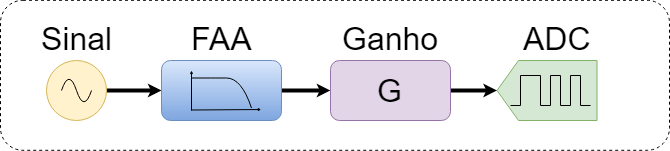
\includegraphics[width=\linewidth]{../Fotos/Diagramas/sinalFaaADC/sinalFaaADC.png}
		\caption{Condicionamento do sinal analógico}
		\label{fig:condicionamentoSinal}
	\end{figure}

	A seguir, serão descritos cada parte que compõe este processo.

	\section{Transdutores piezoelétricos}
		Transdutores piezoelétricos são largamente utilizados para
		monitoramento industrial. Alguns desses transdutores possuem uma eletrônica
		integrada que pré-amplifica e condiciona o sinal para melhor
		desempenho da medição. Os transdutores piezoelétricos com eletrônica
		integrada são denominados IEPE \cite{iepeCircuit}. Entre os transdutores, ou medidores, do tipo IEPE
		mais comuns, encontram-se os transdutores de pressão e de
		aceleração.

		Os medidores IEPE possuem variadas fichas técnicas, com diferentes
		faixas de alimentação, faixas de sinal de saída e tipos de sinal de
		saída. No caso dos medidores de aceleração com saída em tensão, os
		terminais de alimentação e de sinal de saída são compartilhados.

		Os transdutores de aceleração necessitam ser alimentados por uma
		tensão entre $18V$ e $30V$ com uma corrente constante de polarização
		entre $2ma$ e $10ma$, podendo variar de medidor para medidor. Para
		isso, utiliza-se uma fonte de tensão em série com uma fonte de
		corrente. Assim, o sinal de saída é a tensão imediatamente após a
		fonte de corrente. O esquemático abaixo ilustra o circuito elétrico
		equivalente da alimentação de um transdutor IEPE com saída em
		tensão.

		\begin{figure}[H]
			\centering
			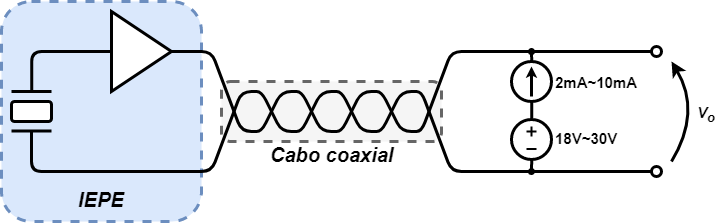
\includegraphics[width=\linewidth]{../Fotos/Diagramas/iepe.png}
			\caption{Diagrama de interligação de um transdutor \textit{IEPE}}
			\label{fig:ligacaoIEPE}
		\end{figure}

		A conversão do sinal de saída para a grandeza de interesse é dada
		por uma relação linear de tensão e da unidade da grandeza. Essa
		relação é denominada sensibilidade. Como exemplo, toma-se o
		transdutor IEPE AC102, que possui sensibilidade de $100mV/g$.
		Assim, com um valor de fundo de escala de $\pm50g$, têm-se variações
		no valor da tensão de saída de $\pm5V$.\cite{ctc}

	\section{O filtro anti-\textit{aliasing} e o teorema da amostragem}
		Seja um sinal $S(t)$ com maior componente de frequência
		$f_{max}$. Segundo o Teorema da Amostragem, ou Teorema de
		\textit{Nyquist}, esse sinal deve ser amostrado com uma
		frequência $f_s$ tal que $f_s>2f_{max}$. Caso contrário, o
		espectro de frequência irá sobrepor-se, impossibilitando a
		reconstrução correta do sinal no tempo. Esse fenômeno é denominado
		de \textit{aliasing} e a frequência $2\*f_{max}$ é definida como
		frequência de \textit{Nyquist}. \cite{nyquist}

		Como exemplo, assume-se o sinal $S(t) = 0,7\*sen(2\*\pi\*50\*t)
		+ sen(2\*\pi\*120\*t)$. O sinal é amostrado com uma frequência
		$f_s = 250Hz$. Os gráficos do sinal original, do sinal
		amostrado e da FFT (\textit{Fast Fourier Transform}), gerada a
		partir da aquisição do sinal na dada frequência de amostragem,
		são exibidos na Figura ~\ref{fig:exemploAliasing250} e foram gerados
		através do \textit{software} Scilab

		Como a maior componente de frequência do sinal $S(t)$ é $120Hz$,
		a frequência de \textit{Nyquist} é $240Hz$. Assim, a taxa de
		amostragem satisfaz o Teorema da Amostragem. Com isso possibilita-se
		uma correta visualização da FFT e da reconstrução do sinal no tempo.

		Ao fazer uma segunda aquisição do mesmo sinal com uma taxa de
		amostragem $f_s = 200Hz$, obtém-se os gráficos exibidos na
		Figura ~\ref{fig:exemploAliasing200}. Como a frequência de amostragem
		é menor que a frequência de \textit{Nyquist} para este sinal, ocorre
		\textit{aliasing} e o sinal não é reconstruído corretamente.
		Esse erro também pode ser visto pela FFT, que apresenta
		frequências diferentes do sinal original.

		\newpage

		\begin{figure}[!ht]
			\centering
			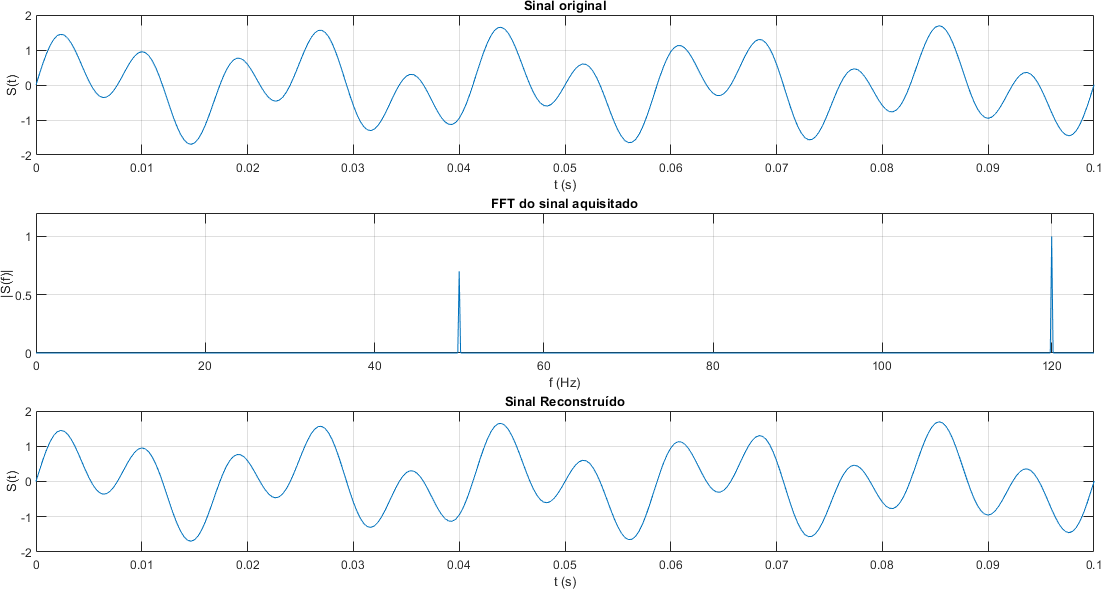
\includegraphics[width=\linewidth]{../Fotos/aliasingFs250.png}
			\caption{Exemplo de sinal sem \textit{aliasing} amostrado à $250Hz$}
			\label{fig:exemploAliasing250}
		\end{figure}

		\begin{figure}[H]
			\centering
			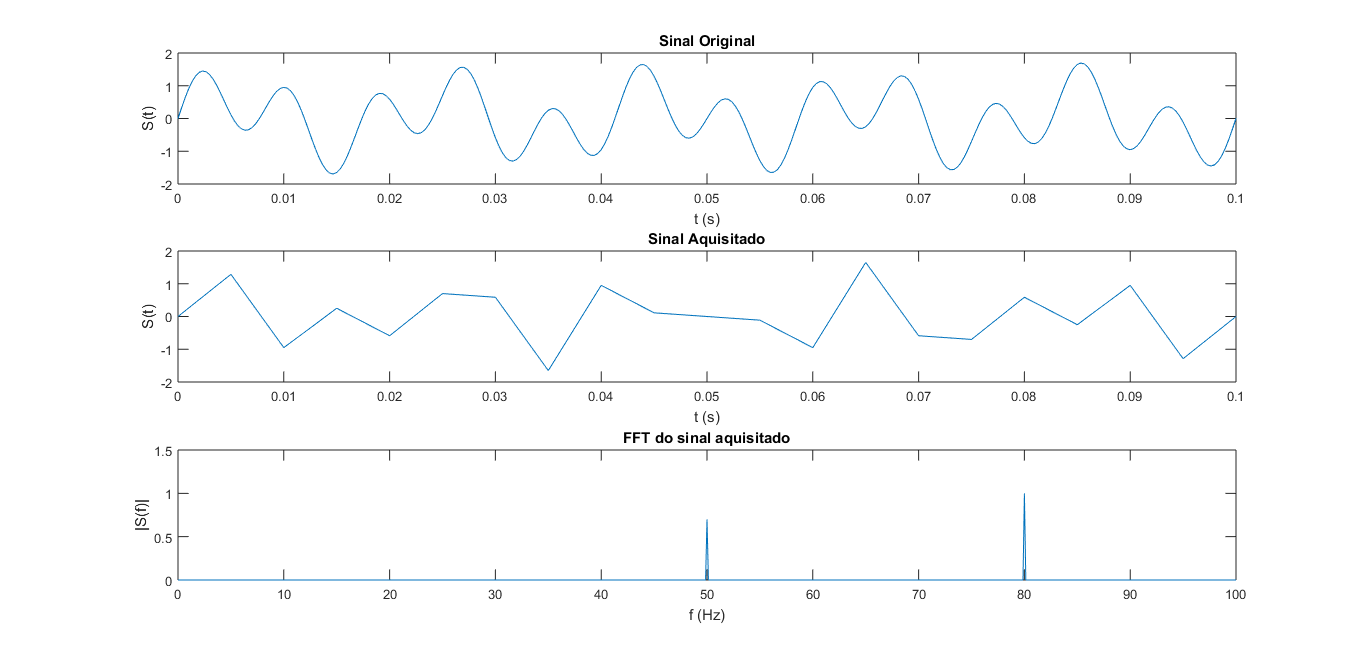
\includegraphics[width=\linewidth]{../Fotos/aliasingFs200.png}
			\caption{Exemplo de sinal com \textit{aliasing} amostrado à $200Hz$}
			\label{fig:exemploAliasing200}
		\end{figure}

		\pagebreak

		O filtro anti-\textit{aliasing} trata-se de um filtro passa-baixa. Um filtro passa-baixa ideal possui
		característica de módulo em frequência mostrada na Figura ~\ref{fig:filtroIdeal}.

		\begin{figure}[!ht]
			\centering
			\begin{minipage}{.4\linewidth}
				\centering
				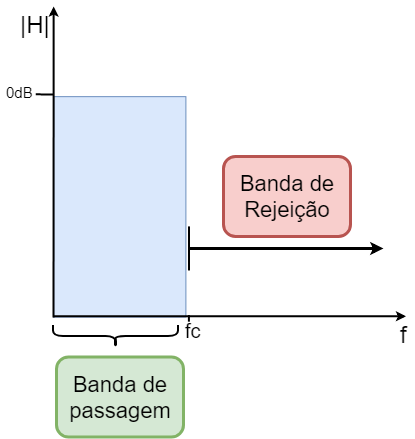
\includegraphics[width=.8\linewidth]{../Fotos/Diagramas/sinalFaaADC/filtroIdeal.png}
				\caption{Resposta em frequência de um filtro ideal}
				\label{fig:filtroIdeal}
			\end{minipage}
			\hfill\vline\hfill
			\begin{minipage}{.4\linewidth}
				\centering
				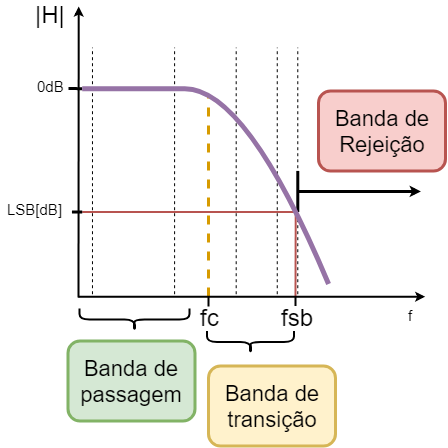
\includegraphics[width=\linewidth]{../Fotos/Diagramas/sinalFaaADC/filtroReal.png}
				\caption{Resposta em frequência de um filtro real}
			\end{minipage}
		\end{figure}

		Entretanto, os filtros passa-baixa reais possuem uma banda a
		mais: a banda de transição. Essa banda representa os sinais de
		frequência cujas amplitudes não foram atenuadas suficientemente,
		de forma que não possam ser lidas pelo Conversor Analógico-Digital
		(ADC). Assim, se forem desprezadas na admissão da taxa de amostragem,
		podem gerar \textit{aliasing}.

		Com isso, em uma primeira análise, pode-se dizer que a frequência de
		amostragem deve satisfazer $f_s>2*f_{sb}$, em que $f_{sb}$ é chamada
		\textit{stop band frequency}, ou frequência da banda de rejeição.

		Assim, pode-se dimensionar a ordem de um filtro anti-\textit{aliasing} a partir do número de bits de seu conversor ADC. A banda de rejeição é caracterizada por ter atenuação
		suficiente para que as frequências inseridas naquela banda possuam amplitude
		inferior ao LSB do ADC. Logo, o ganho na banda de rejeição $H(f_{SB})$ é
		dado por:
		\begin{gather*}
			H(f_{SB}) = LSB/V_{o(max)}\\
			H(f_{SB}) = \frac{LSV}{2^n\times LSV}\\
			H(f_{SB}) = 2^{-n}V/V\\
			ou\\
			H(f_{SB})_{[dB]} = -20\*log(2^n) dB
		\end{gather*}
		Em que $n$ é o número de bits do conversor ADC. Assim, para $n=12$, têm-se que a atenuação para a banda de rejeição deve ser de:
		\begin{gather*}
			H(f_{SB})_{[dB]} = -72,25 dB
		\end{gather*}
		Os filtros analógicos, a partir da frequência de corte $f_c$, possuem atenuação dada por:
		\begin{gather*}
			H(f) = -m\times 20 dB/dec, para f>f_c
		\end{gather*}
		Em que $m$ é um número inteiro diferente de zero e representa a ordem do filtro. Logo, se a banda de transição deve ser igual a uma década e a atenuação na banda de rejeição deve ser de $-72,25 dB$, então a ordem do filtro deve ser de, no mínimo:
		\begin{gather*}
			m = -\frac{H(f_sb)}{20 dB/dec} = 3,6\\
			m = 4
		\end{gather*}

		Não existe método capaz de reverter o \textit{aliasing} após o
		sinal ser amostrado. Então, o que deve ser feito é assumir uma
		faixa de frequência de interesse e utilizar circuitos capazes de
		atenuar frequências acima da frequência de \textit{Nyquist}.
		Essa atenuação deve ser tal que o ADC não possua resolução capaz
		de detectar as componentes de alta frequência. Os circuitos
		responsáveis por garantir que não ocorra \textit{aliasing} são
		denominados filtro anti-\textit{aliasing} (FAA).

	\section{Conversor analógico-digital}
		O conversor analógico-digital, ou ADC, é responsável por digitalizar
		um sinal analógico. A conversão é referenciada às tensões de alimentação
		do ADC e graduada de acordo com o número de \textit{bits} \cite{artElectronics}. Como exemplo,
		um conversor alimentado por uma tensão de $5V$ e com $10$ \textit{bits} de
		resolução possui $2^{10}$ divisões. Assim, a menor divisão do conversor é
		de $5/2^{10} = 4,88mV$ e, consequentemente, este é o menor valor que pode
		ser detectado pelo ADC. Se a resolução fosse de $12$ \textit{bits} ao invés
		de $10$ \textit{bits}, a resolução do conversor seria de $5/2^{12}=1,22mV$.
		Este também é o passo do conversor, também definido como LSB
		(\textit{Least Significant Bit}), ou seja, todas os valores digitalizados
		são múltiplos da resolução.
%#Endregion

% ----------------------------------------------------------
%#Region Capítulo 3 - Materiais, Métodos e Desenvolvimento
% ----------------------------------------------------------
\chapter{Materiais, Métodos e Desenvolvimento}
	\section{Levantamento de requisitos}
		Os sensores de vibração que serão utilizados são do modelo CTC AC102, cedidos pela empresa supervisora. Estes acelerômetros necessitam de uma corrente de excitação fixa, além da alimentação. Tal sensor irá basear o projeto do circuito de condicionamento do sinal.
		
		As principais características do transdutor AC102 são apresentadas
		abaixo.\cite{ctc}
		
		\begin{itemize}
			\item Sensibilidade: $100mV/g$
			\item Tensão de alimentação: $18 - 30 VDC$
			\item Faixa de operação: $\pm 50g$
			\item Corrente de excitação: $2 - 10mA$
			\item Tensão de saída polarizada: $10 - 14 VDC$
			\item Faixa de passagem: $1 - 10.000 Hz$
		\end{itemize}

		Abaixo, são descritos os principais requisitos do projeto.

		\begin{itemize}
			\item O sistema deve ser capaz de amostrar dados de vibração da
			estrutura e enviar remotamente para um módulo receptor conectado a um computador. O alcance
			deve ser superior à 20 metros em área livre. Em geral, essa é a distância em que é possível posicionar-se um computador em relação ao ponto de medição.
			
			\item Possuir quatro canais com entradas para conectores BNC. Estes são os conectores padrão dos medidores IEPE e também do transdutor AC 102. Com quatro canais, torna-se possível realizar a medição de um ponto de forma triaxial ou medir o desbalanceamento de uma peneira com quatro pontos de medição.
			
			\item Ser capaz de amostrar sinais de $250Hz$ com uma resolução de $100mg$, sendo $g$
			a aceleração da gravidade. Tal frequência abrange praticamente todas as medições de máquinas de grande porte, as quais possuem constantes de tempo muito elevadas.
			
			\item Ser capaz de operar por 2h com um \textit{powerbank} modelo CB078 com saída de $5V$
			e capacidade de $2200mAh$. A utilização de um \textit{powerbank} não só facilita e reduz custos do projeto como também permite que o sistema possa ser utilizado diretamente no computador, nos casos em que a telemetria não é necessária.
			
		\end{itemize}

	\section{Análise de requisitos}
	
		A partir dos requisitos, a placa deve possuir, essencialmente, uma
		ou mais fontes reguláveis, um ou mais conversores ADC, unidades de lógica programável
		e sistemas de telemetria.

		Considerando uma eficiência de $80\%$ do conversor DC/DC interno do
		\textit{powerbank}, a capacidade total do modelo CB078 é admitida como sendo
		1760mAh. Assim, para operar durante 2h o sistema deve ter consumo de
		corrente inferior a 880mA e possuir tensão de alimentação de $5V$.

		A alimentação do sensor deve ser de $18V$ a $30V$. Como a entrada de
		alimentação do sistema é de $5V$, optou-se por alimentar o sensor
		piezoelétrico com $19V$ utilizando uma fonte chaveada \textit{boost}, que será
		descrita mais à frente.

		A fonte de corrente deve possuir valor de corrente de $2mA$ a $10mA$. Um valor muito
		utilizado comercialmente é $4mA$, por ter um consumo intermediário e não trabalhar
		muito próximo dos valores máximos e mínimos absolutos.

		Quando excitado, o medidor IEPE possui tensão média de saída entre $10V$ e $14V$. Com uma tensão média de, por exemplo, $12V$, o sinal de $\pm 5V$ irá excursionar de $7V$ a $17V$. Assim, como o sinal varia sobre uma tensão positiva, não há a necessidade de utilização de fontes simétricas. Dessa forma, o filtro
		anti-\textit{aliasing} deve possuir amplificadores operacionais	capazes de operar com alimentação não-simétrica de 19V.
		
		Todos os valores acima citados definem as condições de contorno do
		projeto a ser desenvolvido.	

	\section{Dimensionamento do ADC}
		
		As condições de contorno do projeto impõem uma resolução de $100mg$. Como
		visto na análise de requisitos e no diagrama da Figura ~\ref{fig:condicionamentoSinal},
		têm-se os seguintes dados.
		\begin{itemize}
			
			\item Tensão média de entrada: $V_{i(av)} = 12V$;
			\item Excursão total do sinal ($\pm5V$): $V_{i(pp)} = 10V$.
			
		\end{itemize}
		Assim, as tensões após o FAA e o bloco de ganho são:

		\begin{itemize}	
			\item Tensão média de saída: $V_{o(av)} = G\* V_{i(av)}$;
			\item Tensão máxima de saída: $V_{o(max)} = G\* (V_{i(av)} + \frac{V_{i(pp)}}{2})$;
		\end{itemize}	
			
		Assim, calculou-se o ganho e o número mínimo de bits do conversor ADC para satisfazer as condições de contorno especificadas. O desenvolvimento matemático pode ser visto no Apêndice ~\ref{ape:calculoADC}.

		\begin{itemize}	
			\item $n = 12 bits$
			\item $G = 0,1737 V/V$, se a tensão de alimentação do ADC for de $3,3V$
			\item $G = 0,263 V/V$, se a tensão de alimentação do ADC for de $5V$
		\end{itemize}	

	\section{Dimensionamento do FAA}

		A banda de rejeição é caracterizada por ter atenuação
		suficiente para que as frequências inseridas naquela banda possuam amplitude
		inferior ao LSB do ADC. Como já calculado anteriormente, $n=12$. Assim:
		\begin{gather*}
			H(f_{SB})_{[dB]} = -72,25 dB
		\end{gather*}

		Os ensaios de vibração que se baseia o projeto, apresenta na maior parte do tempo, excitações de frequência fixa com eventuais picos. O que
		interessa para a análise da estrutura é se a amplitude em
		determinada frequência é maior que a prevista no modelo. Ou se a
		estrutura sofreu algum impacto cuja amplitude ultrapassa determinado
		valor. Como é desejada uma baixa frequência de amostragem, o filtro deve possuir uma rápida atenuação em frequência. Nesses casos, variações próximas a até $10\%$ na amplitude não interferem na medição. Ou seja, \textit{ripple} de até $1dB$ na banda de passagem é aceitável.

		Com isso, optou-se pelo filtro de topologia
		\textit{Chebyshev}, que apresenta rápido decaimento na banda de transição em troca de oscilações na banda de passagem. O filtro ainda é caracterizado por ser de sexta ordem, com
		frequência de corte de $265Hz$. Esta frequência foi escolhida um
		pouco acima da frequência de interesse, que é se $250Hz$.

		Os amplificadores operacionais utilizados no FAA devem
		possuir \textit{offset} de tensão cumulativo aos quatro CIs
		menor que $LSB$. No pior caso, em que o ADC opera com $3,3V$,
		o \textit{offset} de cada CI (Circuito Integrado) não pode ser
		maior que $201,4\mu V$. Além disso devem permitir alimentação
		não simétrica de até $19V$.O amplificador operacional OP07CDR atende à tais especificações com um \textit{offset} típico de $60\mu V$.

		Para o projeto do filtro, utilizou-se o \textit{software}
		FilterPro\textsuperscript{TM} da Texas
		Instruments\textsuperscript{TM}. As Figuras ~\ref{fig:circuitoFAA},
		~\ref{fig:faaDiagramaBode} e ~\ref{fig:faaDiagramaBodeZoom} apresentam o
		circuito recomendado para o filtro passa-baixa de 6ª ordem
		\textit{Chebyshev} com topologia \textit{Sallen Key} de ganho
		unitário, frequência de corte $f_c = 265Hz$ e frequência de
		rejeição $f_{SB}\simeq 710Hz$.

		\begin{figure}[!ht]
			\centering
			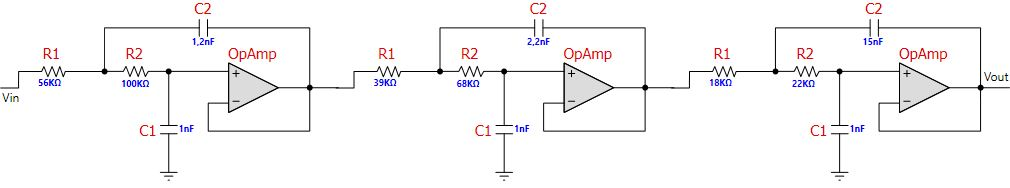
\includegraphics[width=\linewidth]{../Fotos/filterPro.png}
			\caption{Filtro anti-\textit{aliasing}}
			\label{fig:circuitoFAA}
		\end{figure}

		\begin{figure}[!ht]
			\centering
			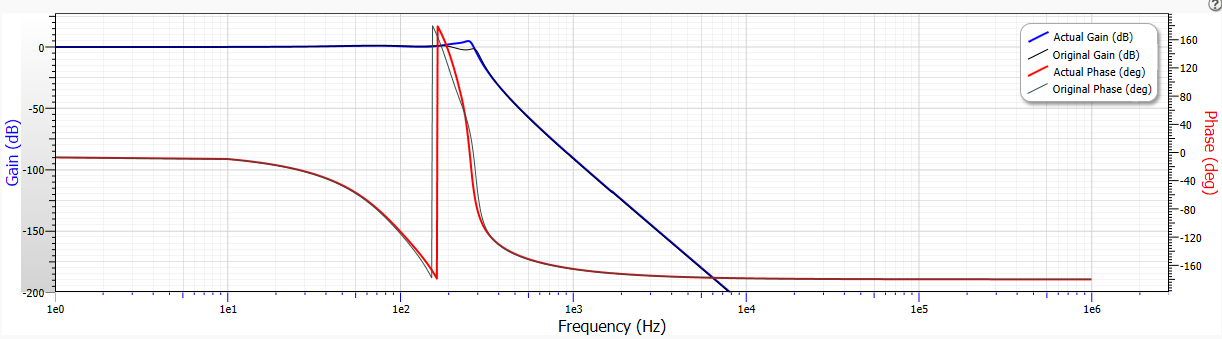
\includegraphics[width=\linewidth]{../Fotos/filterProGF.png}
			\caption{Diagrama de Bode do FFA}
			\label{fig:faaDiagramaBode}
		\end{figure}

		\begin{figure}[!ht]
			\centering
			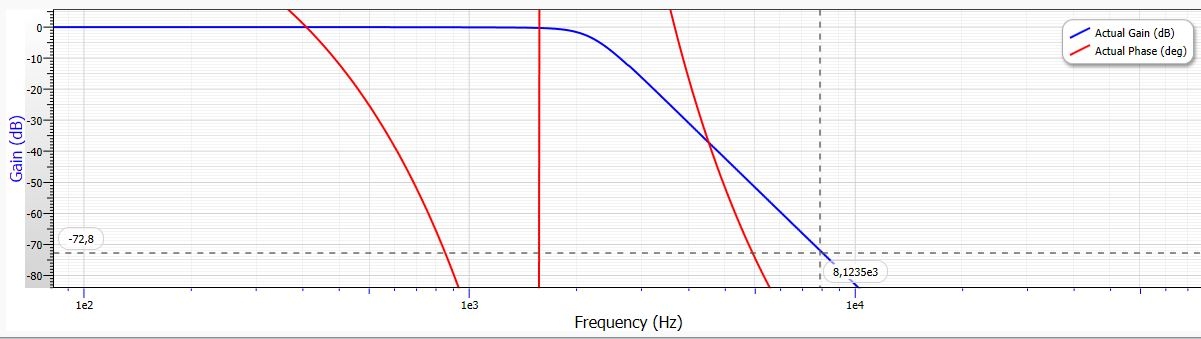
\includegraphics[width=\linewidth]{../Fotos/filterProZoom.png}
			\caption{\textit{Zoom} na banda de transição}
			\label{fig:faaDiagramaBodeZoom}
		\end{figure}

		Após o FAA, o nível do sinal é atenuado para valores abaixo de
		3,3V por meio do ganho $G$. Como já citado anteriormente (Apêndice ~\ref{ape:calculoADC}), para
		alimentação do ADC igual a 3,3V, o ganho deve ser igual a $G =
		0,1737V/V$. Essa relação, dada por um divisor de tensão, pode
		ser aproximada por resistores de $15k\Omega$ e $75k\Omega$, de
		forma que:
		\begin{gather*}
			G = \frac{15k}{15k+75k} = 0,1667V/V
		\end{gather*}

		Como já mostrado (Apêndice ~\ref{ape:calculoADC}), o número de \textit{bits} e o FAA independem do valor
		de $G$, sendo que tal variação irá afetar apenas na calibração dos
		canais. Por tal calibração já fazer-se necessária, também é
		dispensável o uso de resistores de precisão, uma vez que cada
		canal será calibrado individualmente.

		A partir da Figura ~\ref{fig:faaDiagramaBodeZoom}, nota-se que a banda de rejeição inicia em
		$\simeq 695Hz$. Assim, pelo teorema da amostragem seria necessária uma amostragem
		de, pelo menos, $1,4kHz$ para que não ocorra \textit{aliasing}. Contudo,
		é indiferente qualquer \textit{aliasing} que apareça fora da banda de interesse.
		Dessa forma, é passível que ocorra \textit{aliasing} de $f=250Hz$ em diante. Tomando
		uma margem de segurança de aproximadamente $50Hz$, uma frequência de amostragem
		de $f_s=1kHz$ não elimina o \textit{aliasing} na banda de rejeição, mas, sim, na banda
		de interesse.

		A tolerância dos resistores e capacitores do FAA influenciam no
		deslocamento para mais ou para menos das frequências de corte e
		de rejeição no diagrama de magnitude. Porém, como foi dado uma
		margem de $15Hz$ para a frequência de corte e de $50Hz$ para o
		início da banda de rejeição, novamente torna-se dispensável a
		utilização de componentes de precisão.
		\newpage

	\section{Fonte de corrente}

		A fonte de corrente usará a topologia da Figura ~\ref{fig:topologiaFonteCorrente}.

		\begin{figure}[!ht]
			\centering
			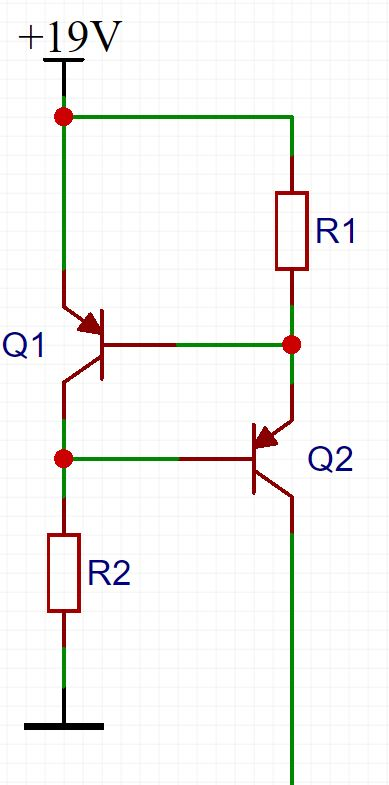
\includegraphics[scale = 0.3]{../Fotos/fonteCorrenteClean2.jpg}
			\caption{Fonte de corrente}
			\label{fig:topologiaFonteCorrente}
		\end{figure}

		A fonte foi dimensionada para fornecer $4mA$ constantes. Os valores foram obtidos por meio do desenvolvimento matemático apresentado no Apêndice ~\ref{ape:calculoCorrente}. Realizou-se um ajuste fino dos valores utilizando o \textit{software} LTSpice.

		Os transistores devem ser transistores de sinal, com
		$V_{be}\simeq 0,7V$. Assim, utilizou-se os transistores BC857B.

		\begin{figure}[!ht]
			\centering
			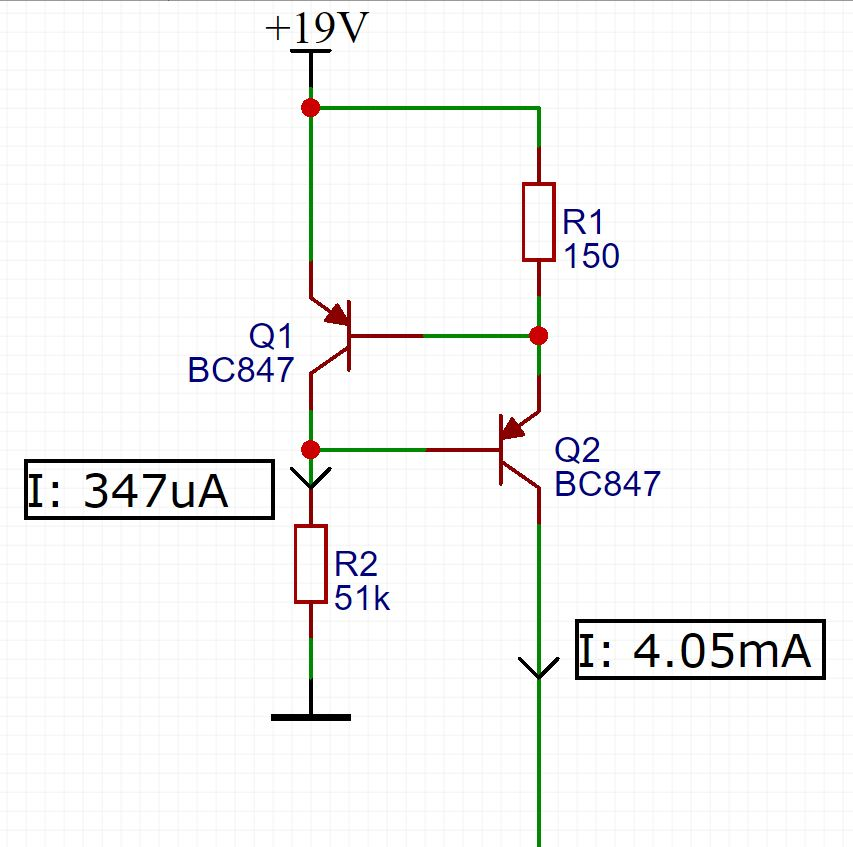
\includegraphics[scale = 0.3]{../Fotos/fonteCorrente2.jpg}
			\caption{Fonte de corrente com medições}
			\label{fig:topologiaFonteCorrenteValores}
		\end{figure}

	\section{Microcontrolador}
		Uma vez definido a taxa de amostragem, a resolução necessária do
		ADC e o número de canais, é possível a escolha do
		microcontrolador e do módulo de telemetria.

		A restrição do ADC de $12$ \textit{bits}, o preço e a ativa comunidade viabiliza a escolha do microcontrolador STM32F103C8T6.\cite{stm}

		O microcontrolador possui características que
		atendem perfeitamente às especificações do projeto. Como
		principais características, pode-se citar:

		\begin{itemize}
			\item Arquitetura de 32 \textit{bits}
			\item $72MHz$ de frequência de \textit{clock} com 1.25 DMIPIS/MHz
			\item 2xADC de $12$ \textit{bits} com até 1MS/s
			\item Tensão de alimentação de $2V$ a $3.6V$
			\item 2xSPI
			\item 3xUSART
			\item 2x$I^2C$
		\end{itemize}

		A capacidade de conversão de até 1MS/s permite que o
		microcontrolador amostre os dados e os transmita para o módulo
		de telemetria em tempo hábil.

		Existem diversas interfaces de programação que podem ser
		utilizadas. A IDE (\textit{Integrated Development Environment })
		disponibilizada gratuitamente pelo fabricante é o \textit{System
		Workbench for STM32}, ou \textit{SW4STM32}, será utilizada.

		Para a programação, utiliza-se o programador ST-Link/V2 que
		conecta USB no computador e faz a interface de programação via
		JTAG.

		Segundo simulações utilizando o \textit{software} STM32CubeMX, o
		microcontrolador possui um consumo médio de $30,56mA$, como pode ser
		visto na Figura ~\ref{fig:consumoSTM}.

		\begin{figure}[!ht]
			\centering
			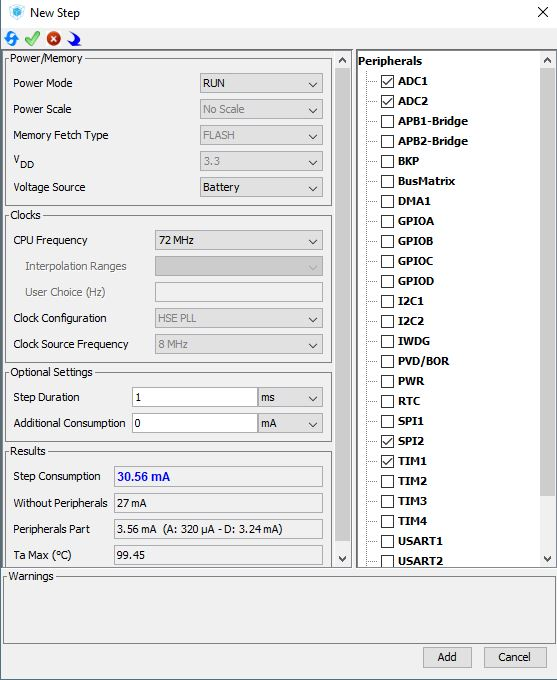
\includegraphics[scale = 0.6]{../Fotos/stmConsumo.jpg}
			\caption{Consumo estimado do STM32F103C8T6}
			\label{fig:consumoSTM}
		\end{figure}

	\section{Telemetria}
		Como cada dado possui $12$ \textit{bits} e cada placa possui um
		máximo de $4$ canais, é necessário que o módulo de telemetria
		tenha uma taxa de transferência de:

		\begin{gather*}
			f_s = 1kHz\\
			Total\:de\:bytes\:por\:amostra = 4\times 12 = 48 bits = 6 bytes\\
			B/s = 6\times 1000 = 6kB/s\\
		\end{gather*}

		O módulo nRF24L01+\cite{nrf} possui taxa de comunicação de até $2Mbps$,
		equivalente a $250kBps$. Outras características do módulo são
		citadas abaixo.

		\begin{itemize}
			\item Frequência de operação de $2,4GHz$
			\item Tensão de alimentação de $1,9V$ a $3,6V$
			\item Half-duplex
			\item Recebe dados de até 6 módulos no mesmo canal
			\item Comunicação SPI de até $10Mbps$
			\item Alcance de comunicação de até $1km$ (ideal)
		\end{itemize}

		Outro ponto importante é que a o rádio utiliza a frequência de $2,4GHz$, a qual pode ser utilizada sem a necessidade de concessão.

		Assim, esse módulo se torna ideal para que a placa receptora consiga
		obter dados de até 6 placas de 4 canais, possibilitando a leitura de
		um total de 24 acelerômetros.

		O nível lógico se adequa ao do microcontrolador bem como a fonte
		de alimentação. Segundo o \textit{datasheet}, o módulo possui
		consumo médio de $40mA$ em transmissão com picos de $115mA$.
		
		\begin{figure}[!ht]
			\centering
			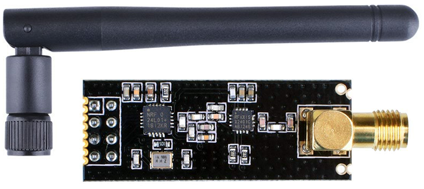
\includegraphics[scale = 0.6]{../Fotos/nrf.png}
			\caption[Módulo nRF24L01+]{Módulo nRF24L01+ \footnotemark}
		\end{figure}

	\section{Fonte Linear}

		A fonte de $3,3V$ deve alimentar o microcontrolador e o módulo de
		telemetria. O consumo total é de menos de $100mA$ na média. Os
		picos de corrente do módulo de telemetria devem ser supridos por
		capacitores posicionados próximos aos terminais de alimentação
		do módulo.
		
		\footnotetext{Acessado(20/10/2019): https://lastminuteengineers.com/wp-content/uploads/2018/07/nRF24L01-PA-LNA-External-Antenna-Wireless-Transceiver-Module.png}

		Como a tensão de alimentação é próxima da tensão a ser regulada,
		optou-se por utilizar um regulador linear ao invés de um
		\textit{buck}. Um \textit{buck} teria uma eficiência em torno de
		$80\%$ enquanto, para essa situação, a eficiência de um regulador
		linear é de $3,3/5 = 66\%$. Devido ao preço e à baixa
		complexidade, escolheu-se o CI AMS1117-3.3 que possui capacidade
		de corrente de $1A$ e requer apenas dois capacitores para
		funcionar.

	\section{Fonte chaveada \textit{boost}}
		Os sensores IEPE operam com uma tensão de alimentação de $18V$ a
		$30V$. A fonte que provê tal alimentação deve ser capaz de
		elevar a tensão de entrada, $5V$, para a tensão desejada e
		alimentar as fontes de corrente dos sensores e o FAA.

		Para o projeto, optou-se pela fonte XL6009 que responsável por regular a tensão de $5V$ para $19V$. O desenvolvimento matemático para conformar as especificações da fonte com as condições de contorno do projeto é apresentado no Apêndice ~\ref{ape:calculoBoost}.

	\section{Consumo total}
		O consumo total é dado pelas cargas das fontes de $19V$ e $3,3V$ e
		suas respectivas eficiências. Assumindo que a eficiência do
		módulo XL6009 como sendo de $75\%$ e que toda a corrente que entra
		na fonte linear é entregue à carga, têm-se que:
		\begin{gather*}
			P = \frac{V_{XL}\times I_{XL}}{\eta _{XL}} + \frac{V_{AMS}\times I_{AMS}}{\eta _{AMS}}\\
			P = \frac{19\times 33,2mA}{0,75} + \frac{3,3\times 70,56mA}{0,66}\\
			P = 1,19W
		\end{gather*}
		Em que o subscrito $XL$ refere-se ao conversor \textit{boost} e
		o subscrito $AMS$ refere-se ao conversor linear.

		O \textit{powerbank} que alimenta a placa possui estimados $1760mAh$ de
		energia. Em \textit{potência-hora}, assumindo uma tensão nominal
		de 5V, a energia total é de 8.8Wh. Assim, a placa consegue operar
		por pouco mais 7h com esse \textit{powerbank}.

	\section{Escolha de componentes}
		Os resistores e capacitores foram escolhidos com os menores
		encapsulamentos disponíveis no mercado brasileiro para compra no varejo:
		0603 e 0805. Isso permite um posicionamento mais preciso de capacitores
		perto dos terminais de alimentação e um melhor acoplamento magnético
		entre os resistores que possam vir a ser influenciados por campos
		magnéticos externos.

	\section{Projeto}
		Para o desenvolvimento da placa, utilizou-se o \textit{software}
		EasyEda \cite{easyEda}. Este ambiente de desenvolvimento de Placas de Circuitos Impressos (PCIs) é gratuito e funciona via navegadores (\textit{browsers}). Possui uma
		vasta biblioteca de \textit{footprints} por operar de forma
		colaborativa, ou seja, todo componente criado por um usuário fica
		disponível para toda comunidade que utiliza a ferramenta.

		O \textit{software} ainda conta com um DRC(\textit{Design Rule
		Check}) básico, que pode analisar trilhas desconectadas, espaçamento
		incorreto entre \textit{pads} e trilhas, entre outras funções.
		\subsection{Esquemático}
			\subsubsection{Fontes}
				Para o conector USB, optou-se pela entrada tipo B, que é a
				mesma utilizada no módulo de aquisição de dados NI-9234.

				Para as fontes, montou-se o esquemático apresentado na Figura ~\ref{fig:esquematicoFontes}.

				\begin{figure}[!ht]
					\centering
					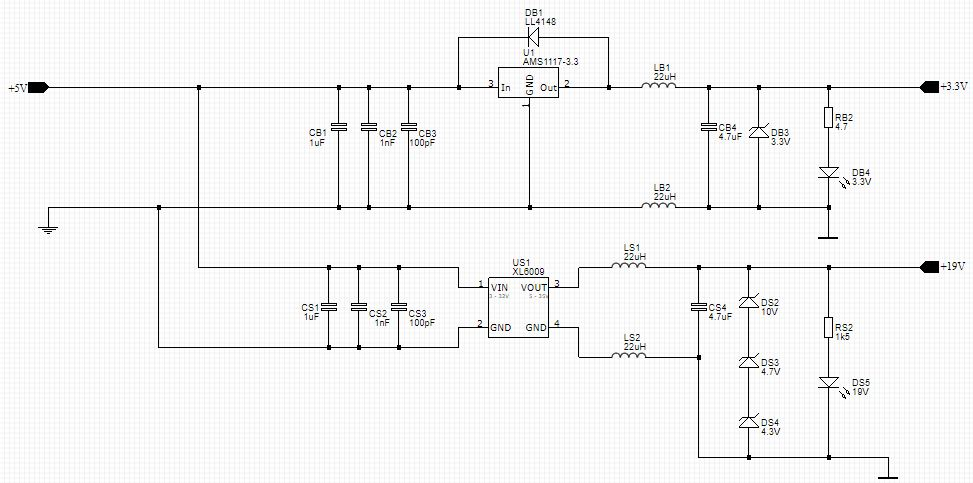
\includegraphics[width=\linewidth]{../Fotos/fonte.jpg}
					\caption{Esquemático das fontes}
					\label{fig:esquematicoFontes}
				\end{figure}

				Os capacitores da entrada filtram oscilações. O filtro LC
				nas saídas das fontes em associação com os zeners possuem
				frequência de corte e de $10kHz$, atenuando o
				\textit{ripple} de altas frequências. Além disso, os
				indutores ainda possuem a função de melhorar o plano de
				terra, isolando o terra da alimentação. É importante
				ressaltar que a frequência de ressonância do circuito LC é
				significativamente menor que a frequência de chaveamento do
				conversor \textit{boost}, que opera em $400kHz$. Isso evita
				instabilidades no sistema.

				O diodo LL4148 atua como diodo grampeador, suprimindo
				possíveis surtos de tensão gerados pelo circuito LC.

				A Figura ~\ref{fig:esquematicoFontesCorrente} apresenta os circuitos das fontes de corrente
				utilizada. O BAV99 atua como grampeador de tensão,
				protegendo a entrada do FAA contra possíveis surtos de
				tensão.

				\begin{figure}[!ht]
					\centering
					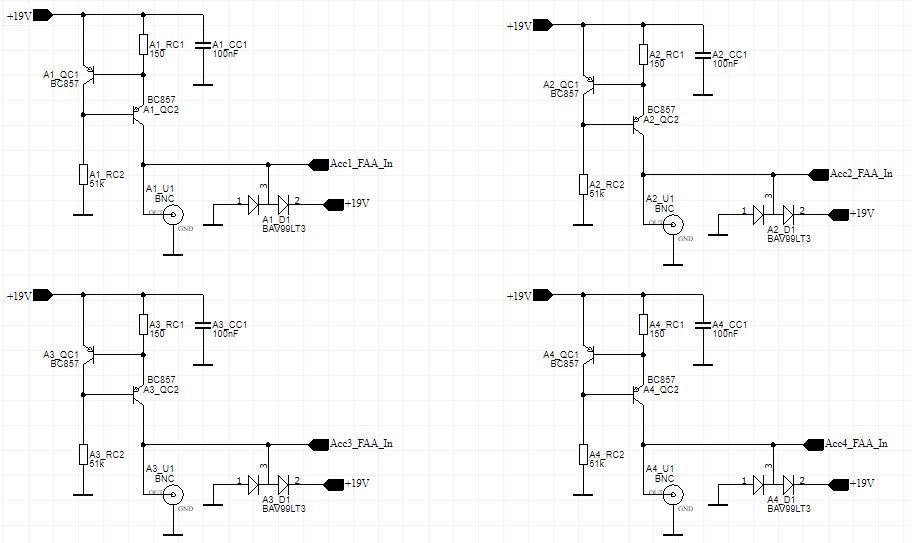
\includegraphics[width=\linewidth]{../Fotos/fonteCorrenteEsquematico.jpg}
					\caption{Esquemático das fontes de corrente}
					\label{fig:esquematicoFontesCorrente}
				\end{figure}				

			\subsubsection{Filtro anti-\textit{aliasing}}

				A Figura ~\ref{fig:esquematicoFAA} apresenta os resistores que compõe o ganho G,
				posicionados na saída do FAA. O BAV99 atua como grampeador,
				protegendo a entrada do ADC.

				Os capacitores de $100nF$ diminuem a influência da
				indutância das trilhas e dos planos de alimentação. O
				capacitor de $1\mu F$ fornece energia em regimes
				transitórios.

				\begin{landscape}
					\vspace*{\fill}
					\begin{center}
						\begin{figure}[!h]
							\centering
							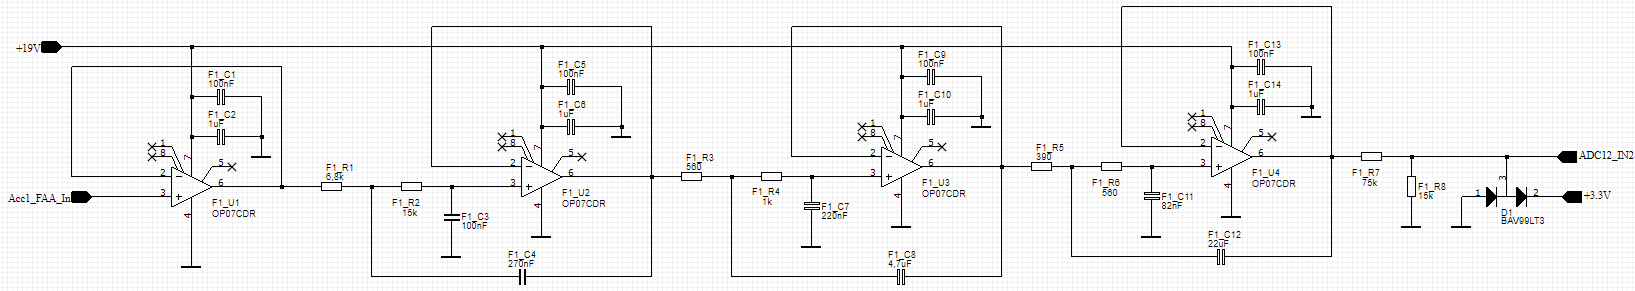
\includegraphics[scale = 0.58]{../Fotos/FAAesquematico.png}
							\caption{Esquemático do filtro anti-\textit{aliasing}}
							\label{fig:esquematicoFAA}
						\end{figure}
					\end{center}
					\vspace*{\fill}
					
				\end{landscape}

			\subsubsection{STM32F103C8T6}

				A Figura ~\ref{fig:esquematicostm} mostra as conexões do STM32F103C8T6. Para a
				alimentação do ADC, acrescentou-se um capacitor de $1nF$ para
				filtrar frequências maiores.

				O cristal de $8MHz$ juntamente com o multiplicador PLL
				(\textit{Phase-Locked Loop}) dentro do microcontrolador
				geram uma frequência de operação do núcleo de $72MHz$.

				Os capacitores de $100nF$ na alimentação diminuem o impacto
				da indutância das trilhas e dos planos de alimentação. Os
				capacitores de $1\mu F$ fornecem energia em regimes
				transitórios.

				Os circuitos compostos pelos transistores Q1 e Q2 são LEDs
				para \textit{debug}.

				\begin{figure}[!ht]
					\centering
					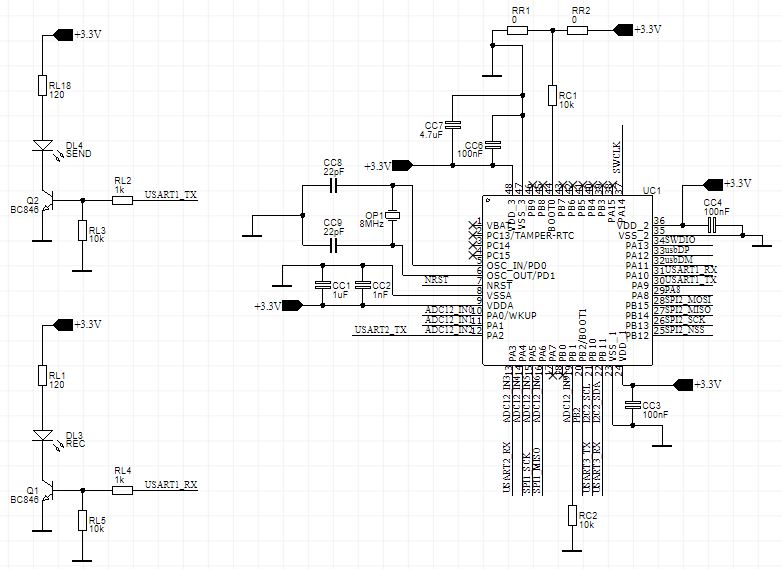
\includegraphics[width=\linewidth]{../Fotos/stmEsquematico.jpg}
					\caption{Esquemático do STM32F103C8T6}
					\label{fig:esquematicostm}
				\end{figure}

			\subsubsection{nRF24L01+}
				A Figura ~\ref{fig:esquematiconrf} apresenta o conjunto de capacitores que são
				conectados próximos à alimentação do módulo de telemetria.
				Utilizou-se dois capacitores de $4,7\mu F$ por serem mais
				baratos e/ou menos volumosos que o mesmo capacitor SMD
				equivalente de tântalo ou eletrolítico. O capacitor de
				$100pF$ atua retirando componentes de frequências de dezenas
				de MHz.

				\begin{figure}[!ht]
					\centering
					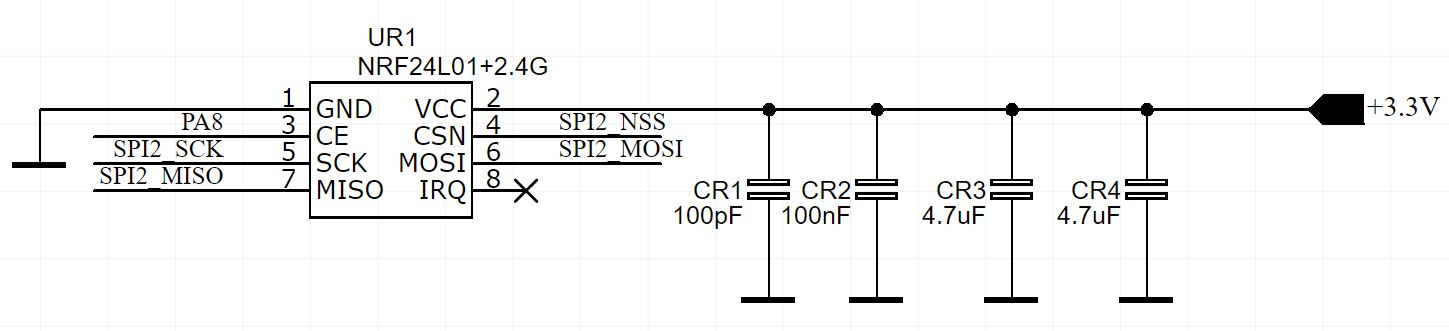
\includegraphics[width=\linewidth]{../Fotos/nrfEsquematico.jpg}
					\caption{Esquemático do nRF24L01+}
					\label{fig:esquematiconrf}
				\end{figure}
				
			\newpage
			\newpage


		\subsection{PCB}
			Para o desenvolvimento do desenho da placa, buscou seguir-se
			os padrões estipulados pela norma IPC-2221A \cite{ipc}.

			A placa foi desenhada em dois \textit{layers}, com componentes
			posicionados em ambos \textit{layers}. Isso possibilita uma redução
			do tamanho total da placa e, consequentemente, do custo. No
			\textit{layer} inferior, utilizou-se um plano de terra a fim de
			diminuir a resistência e indutância do retorno da corrente.
			No \textit{layer} superior utilizou-se dois planos em regiões
			separadas: um \textit{layer} de 19V e outro de $3,3V$, também a fim de
			diminuir a impedância de saída das trilhas de alimentação.

			\begin{figure}[ht]
				\centering
				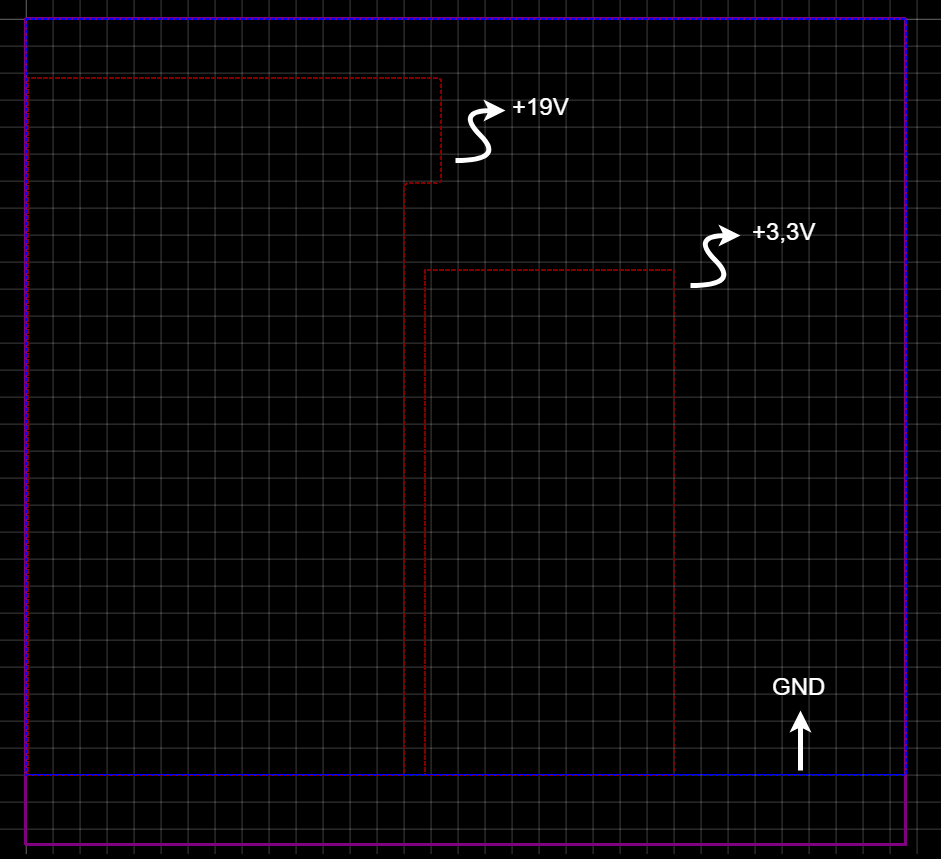
\includegraphics[scale=0.3]{../Fotos/pcbLayers.png}
				\caption{Planos de terra, 19V e 3,3V}
			\end{figure}

			Como pode ser visto na seção 6.2 da norma, como ambos \textit{layers} são
			externos, para uma placa com deposição de cobre de $1oz/ft^2$,
			corrente de $200mA$ e comprimento de $10cm$, a temperatura da
			trilha subiria apenas 1\textdegree C se usado uma espessura de
			trilha de $5,2 mils$, quando em temperatura ambiente de
			25\textdegree C. Assim, para diminuir a queda de tensão terminal e diminuir a indutância das trilhas, optou-se por utilizar trilhas de $8 mils$.

			Os componentes foram posicionados de forma que circuitos
			digitais de alta frequência ficassem distantes de circuitos
			analógicos e que as fontes de alimentação ficassem equidistantes
			da maioria dos circuitos. Isso pode ser visualizado na Figura
			~\ref{fig:analogDigitalFontes}. O microcontrolador por sua vez ficou posicionado de forma
			que estivesse mais próximo dos sinais analógicos, além de evitar
			cruzamento de trilhas.

			\begin{figure}[ht]
				\centering
				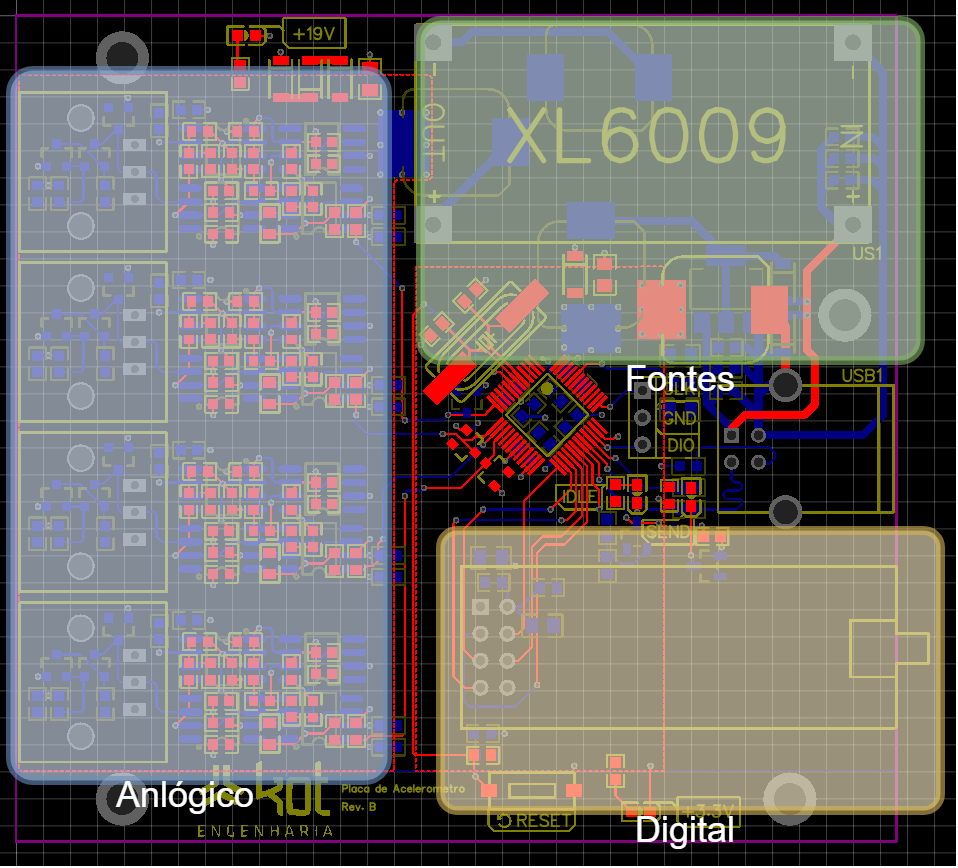
\includegraphics[scale=0.3]{../Fotos/analogDigitalFonte.png}
				\caption{Divisão das partes analógico, digital e fontes}
				\label{fig:analogDigitalFontes}
			\end{figure}

			Os capacitores responsáveis por minimizar os efeitos da
			indutância das trilhas de alimentação foram posicionados o mais
			próximo possível dos semicondutores. Isso minimiza oscilações na
			alimentação devido à surtos de corrente causados pelo módulo de
			telemetria, por exemplo, que possui picos de corrente de até $115mA$.

			\begin{figure}[H]
				\centering
				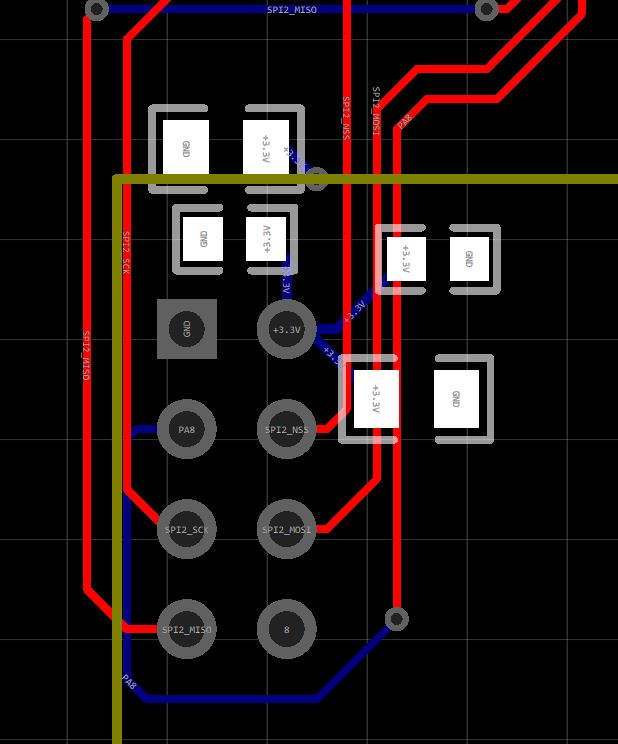
\includegraphics[scale = 0.5]{../Fotos/capNrf.jpg}
				\caption{Capacitores próximos aos pinos de alimentação}
			\end{figure}

			No posicionamento dos componentes do FAA, orientou-se os
			resistores e amplificadores operacionais na mesma direção. Dessa
			forma, eventuais campos magnéticos são anulados por induzirem o
			mesmo ruído em todo o circuito do filtro.

			\begin{figure}[H]
				\centering
				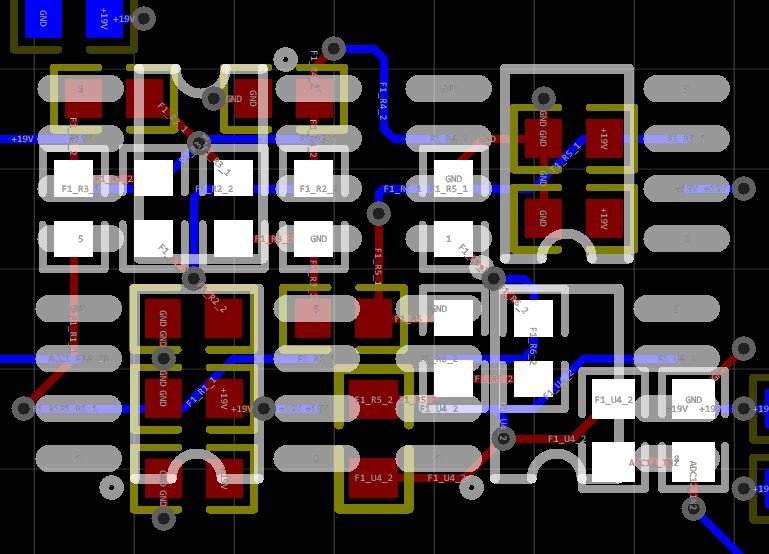
\includegraphics[scale = 0.5]{../Fotos/resAmp.jpg}
				\caption{Resistores e amplificadores operacionais orientados na mesma direção}
			\end{figure}

			A Figura ~\ref{fig:placaFinal} apresenta uma vista geral da placa. Com dimensões de
			$88,8mmx77,72mm$, o preço de produção de 10 placas fica em torno de
			U\$90 ou U\$9 por placa.

			\begin{figure}[H]
				\centering
				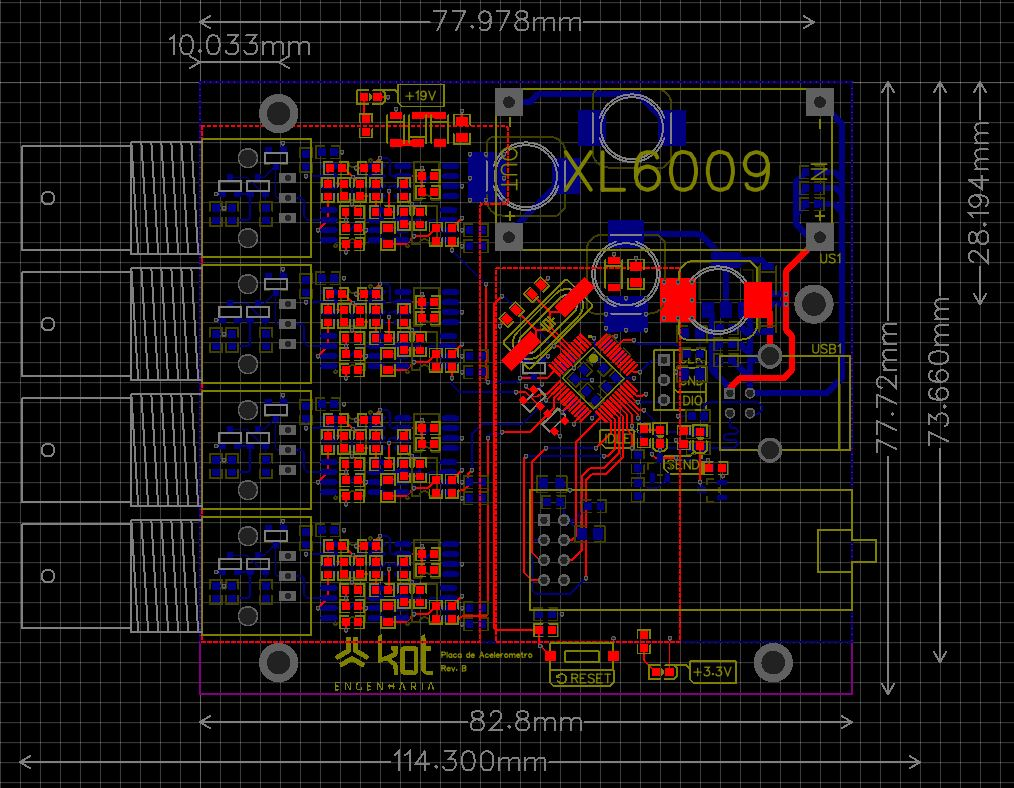
\includegraphics[width=\linewidth]{../Fotos/placaTotal.jpg}
				\caption{Placa final}
				\label{fig:placaFinal}
			\end{figure}

			\newpage

		\subsection{Fabricação e solda}
			A placa foi encomendada pelo site \textit{JLCPCB}. A compra de componentes suficientes para a montagem de 5 placas totalizou aproximadamente 300 reais.

			\begin{figure}[H]
				\centering
				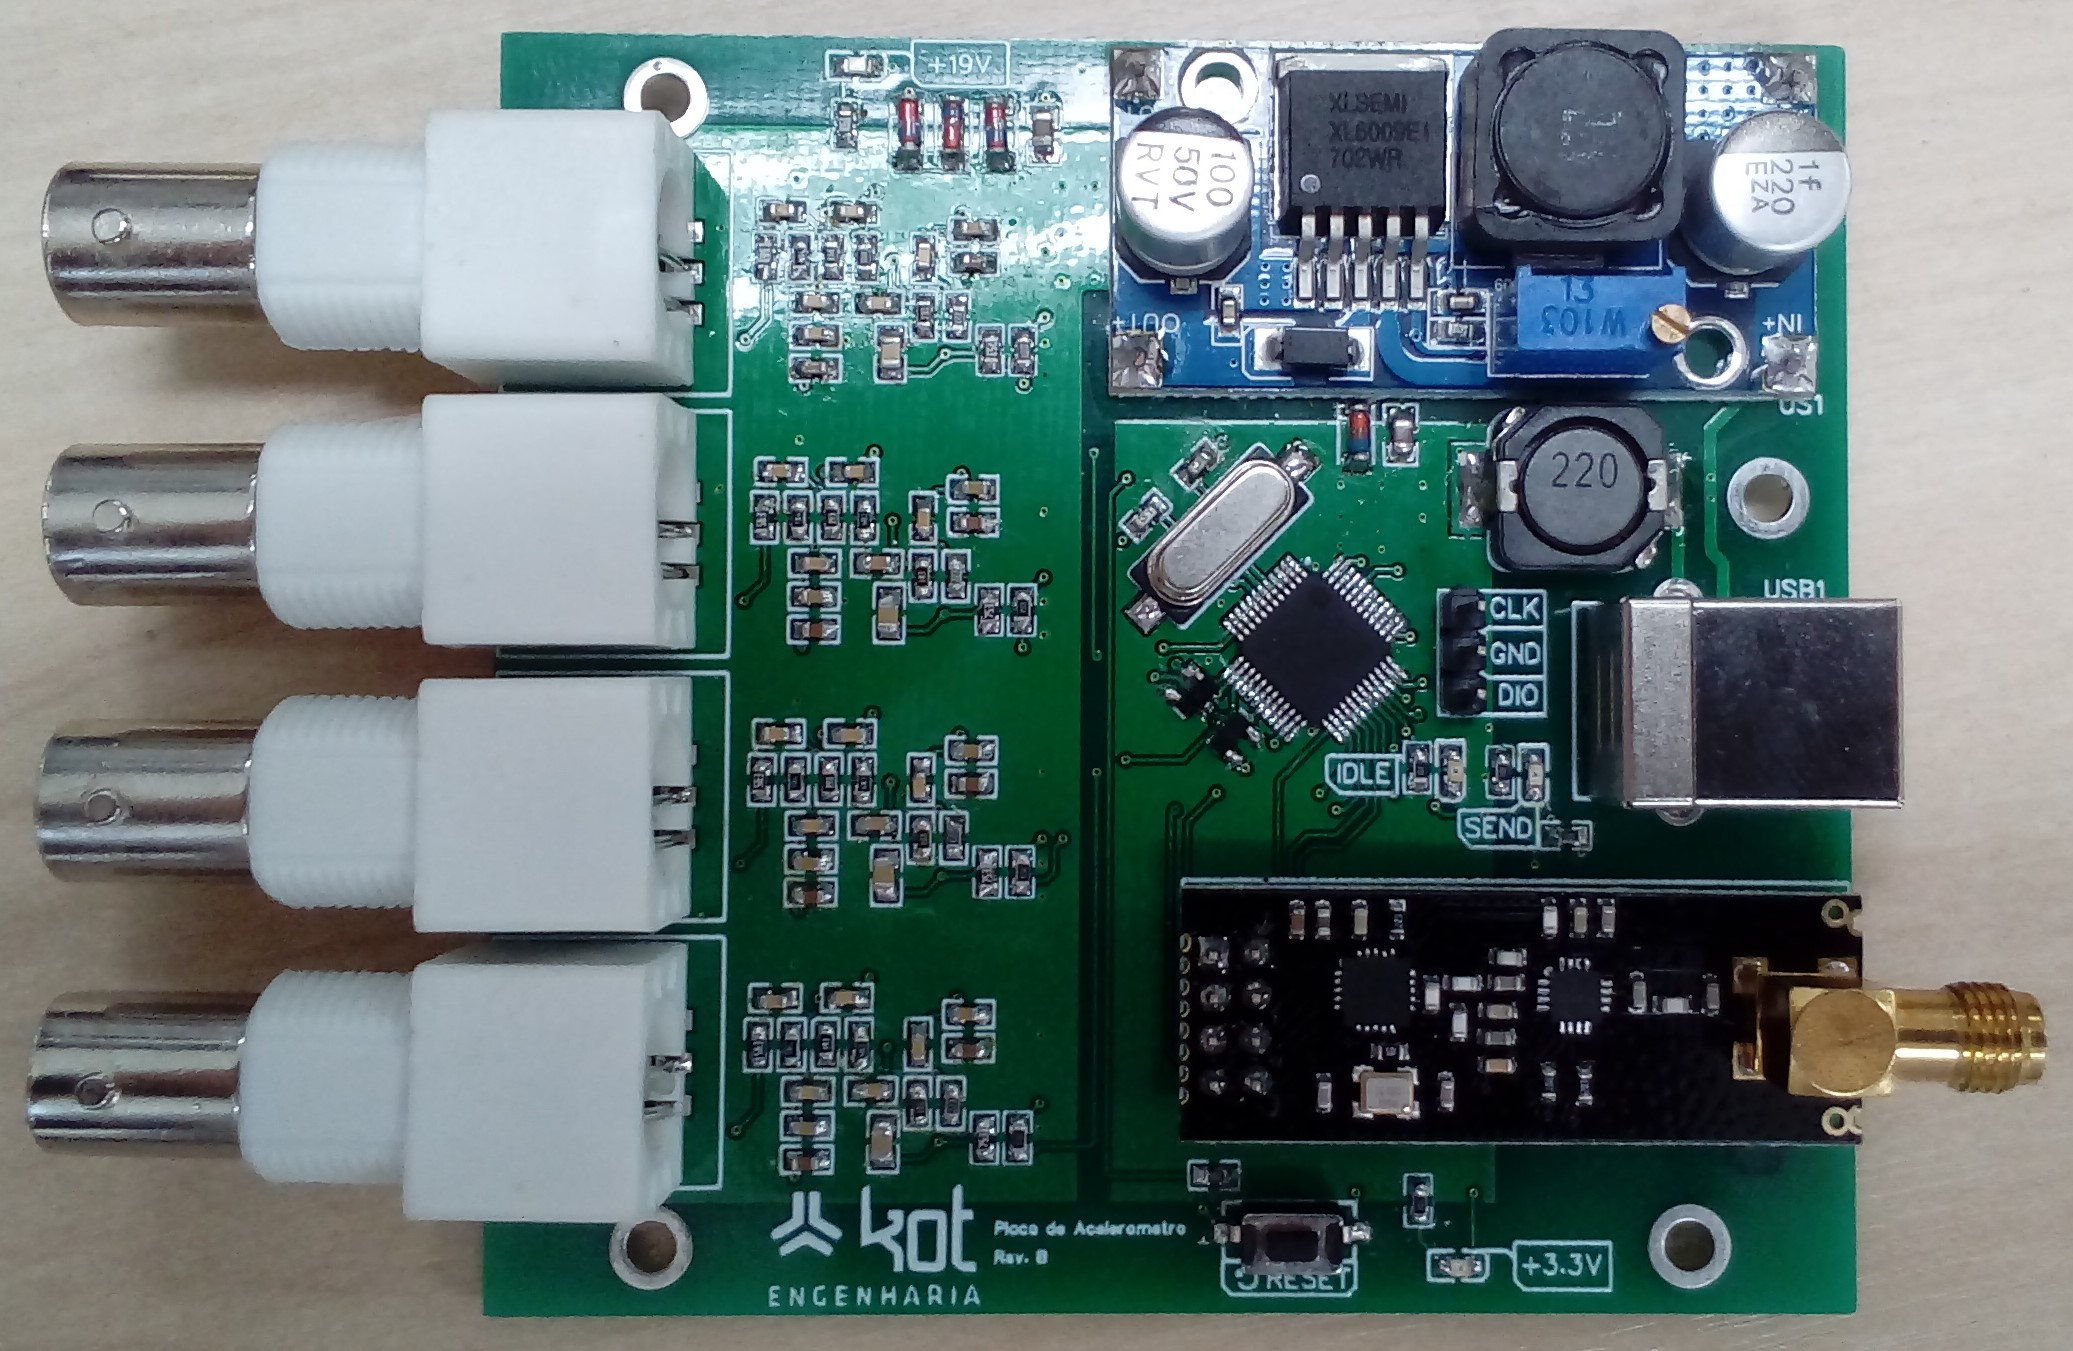
\includegraphics[width=\linewidth]{../Fotos/vistaSuperior.jpg}
				\caption{Vista superior}
			\end{figure}
		\newpage

	\section{NI-9234}
		Por fim, para realização dos ensaios, utilizou-se o módulo NI-9234 como referência de medição. Abaixo, as principais características do módulo, conforme \textit{datasheet}\cite{ni9234}:

		\begin{itemize}
			\item 4 canais
			\item Acoplamento AC ou DC
			\item $24$ \textit{bits} de resolução
			\item Frequência mínima de amostragem de $1kHz$
		\end{itemize}
%#Endregion

% ----------------------------------------------------------
%#Region Capítulo 4 - Resultados
% ----------------------------------------------------------
\chapter{Resultados}
	Foi realizado um ensaio em uma peneira de minério de pequeno
	porte com o objetivo de avaliar se a placa mede os valores corretos
	de amplitude de aceleração. O ensaio e os resultados serão
	apresentados nas seções seguintes.

	Não será possível descrever os códigos desenvolvidos por
	questões da quantidade de linhas geradas. Para ilustrar e sumarizar a rotina do módulo,
	a Figura ~\ref{fig:FSM} apresenta a máquina de estados finitos simplificada do
	microcontrolador.

	\begin{figure}[!ht]
		\centering
		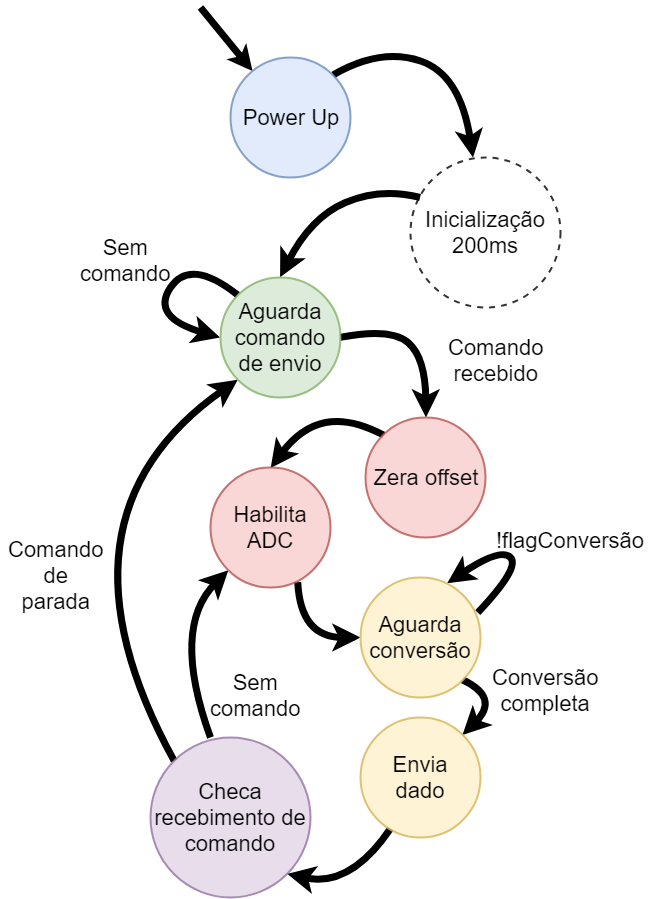
\includegraphics[scale = .47]{../Fotos/diagramaTelemetria.png}
		\caption{Máquina de estados finitos}
		\label{fig:FSM}
	\end{figure}

	\section{Níveis de tensão}
		\subsection{Reguladores de tensão}
			A fim de caracterizar a eficácia do filtro LC
			posicionado na saída dos reguladores de tensão, utilizou-se o
			osciloscópio Tektronix TBS1052B com acoplamento AC medindo o
			potencial entre os terminais antes e após o filtro. Os
			resultados são apresentados nas figuras seguintes.

			\begin{figure}[!ht]
				\centering
				\begin{minipage}{0.4\linewidth}
					\centering
					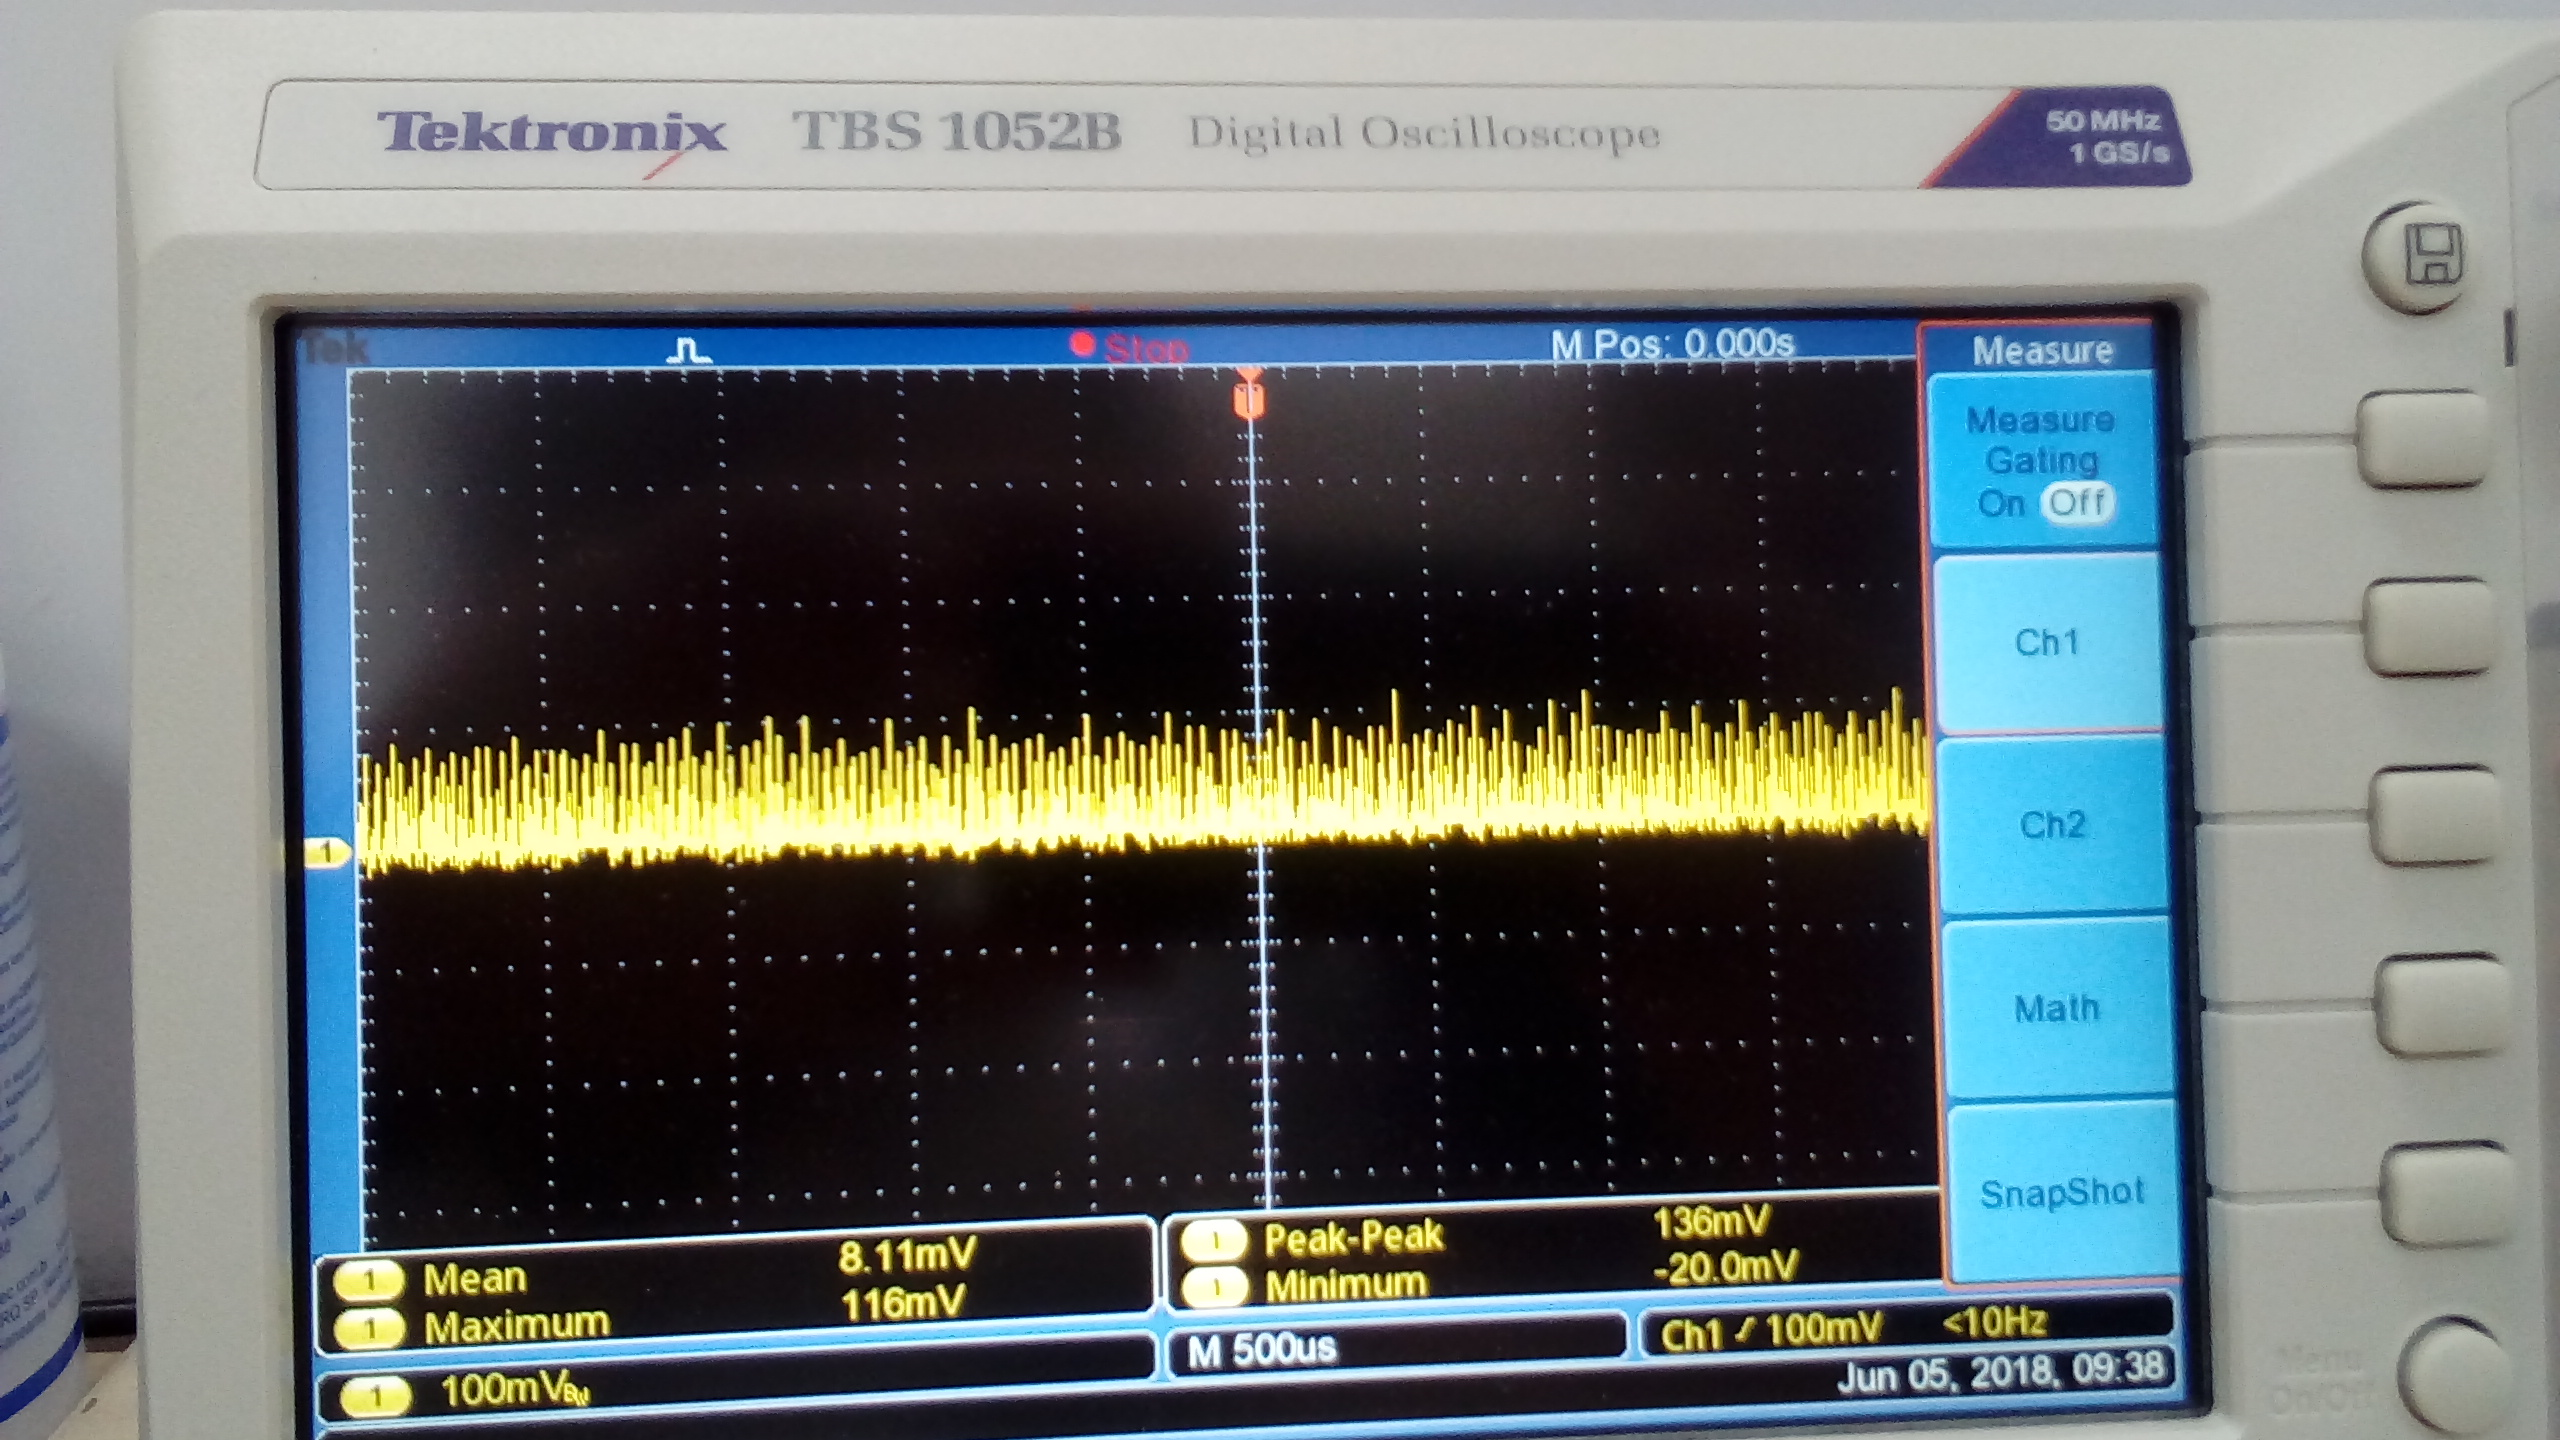
\includegraphics[width = \linewidth]{../Fotos/antesFiltro33.jpg}
					\caption{Sinal AC da saída da fonte de 3,3V}
				\end{minipage}
				\hfill\vline\hfill
				\begin{minipage}{0.4\linewidth}
					\centering
					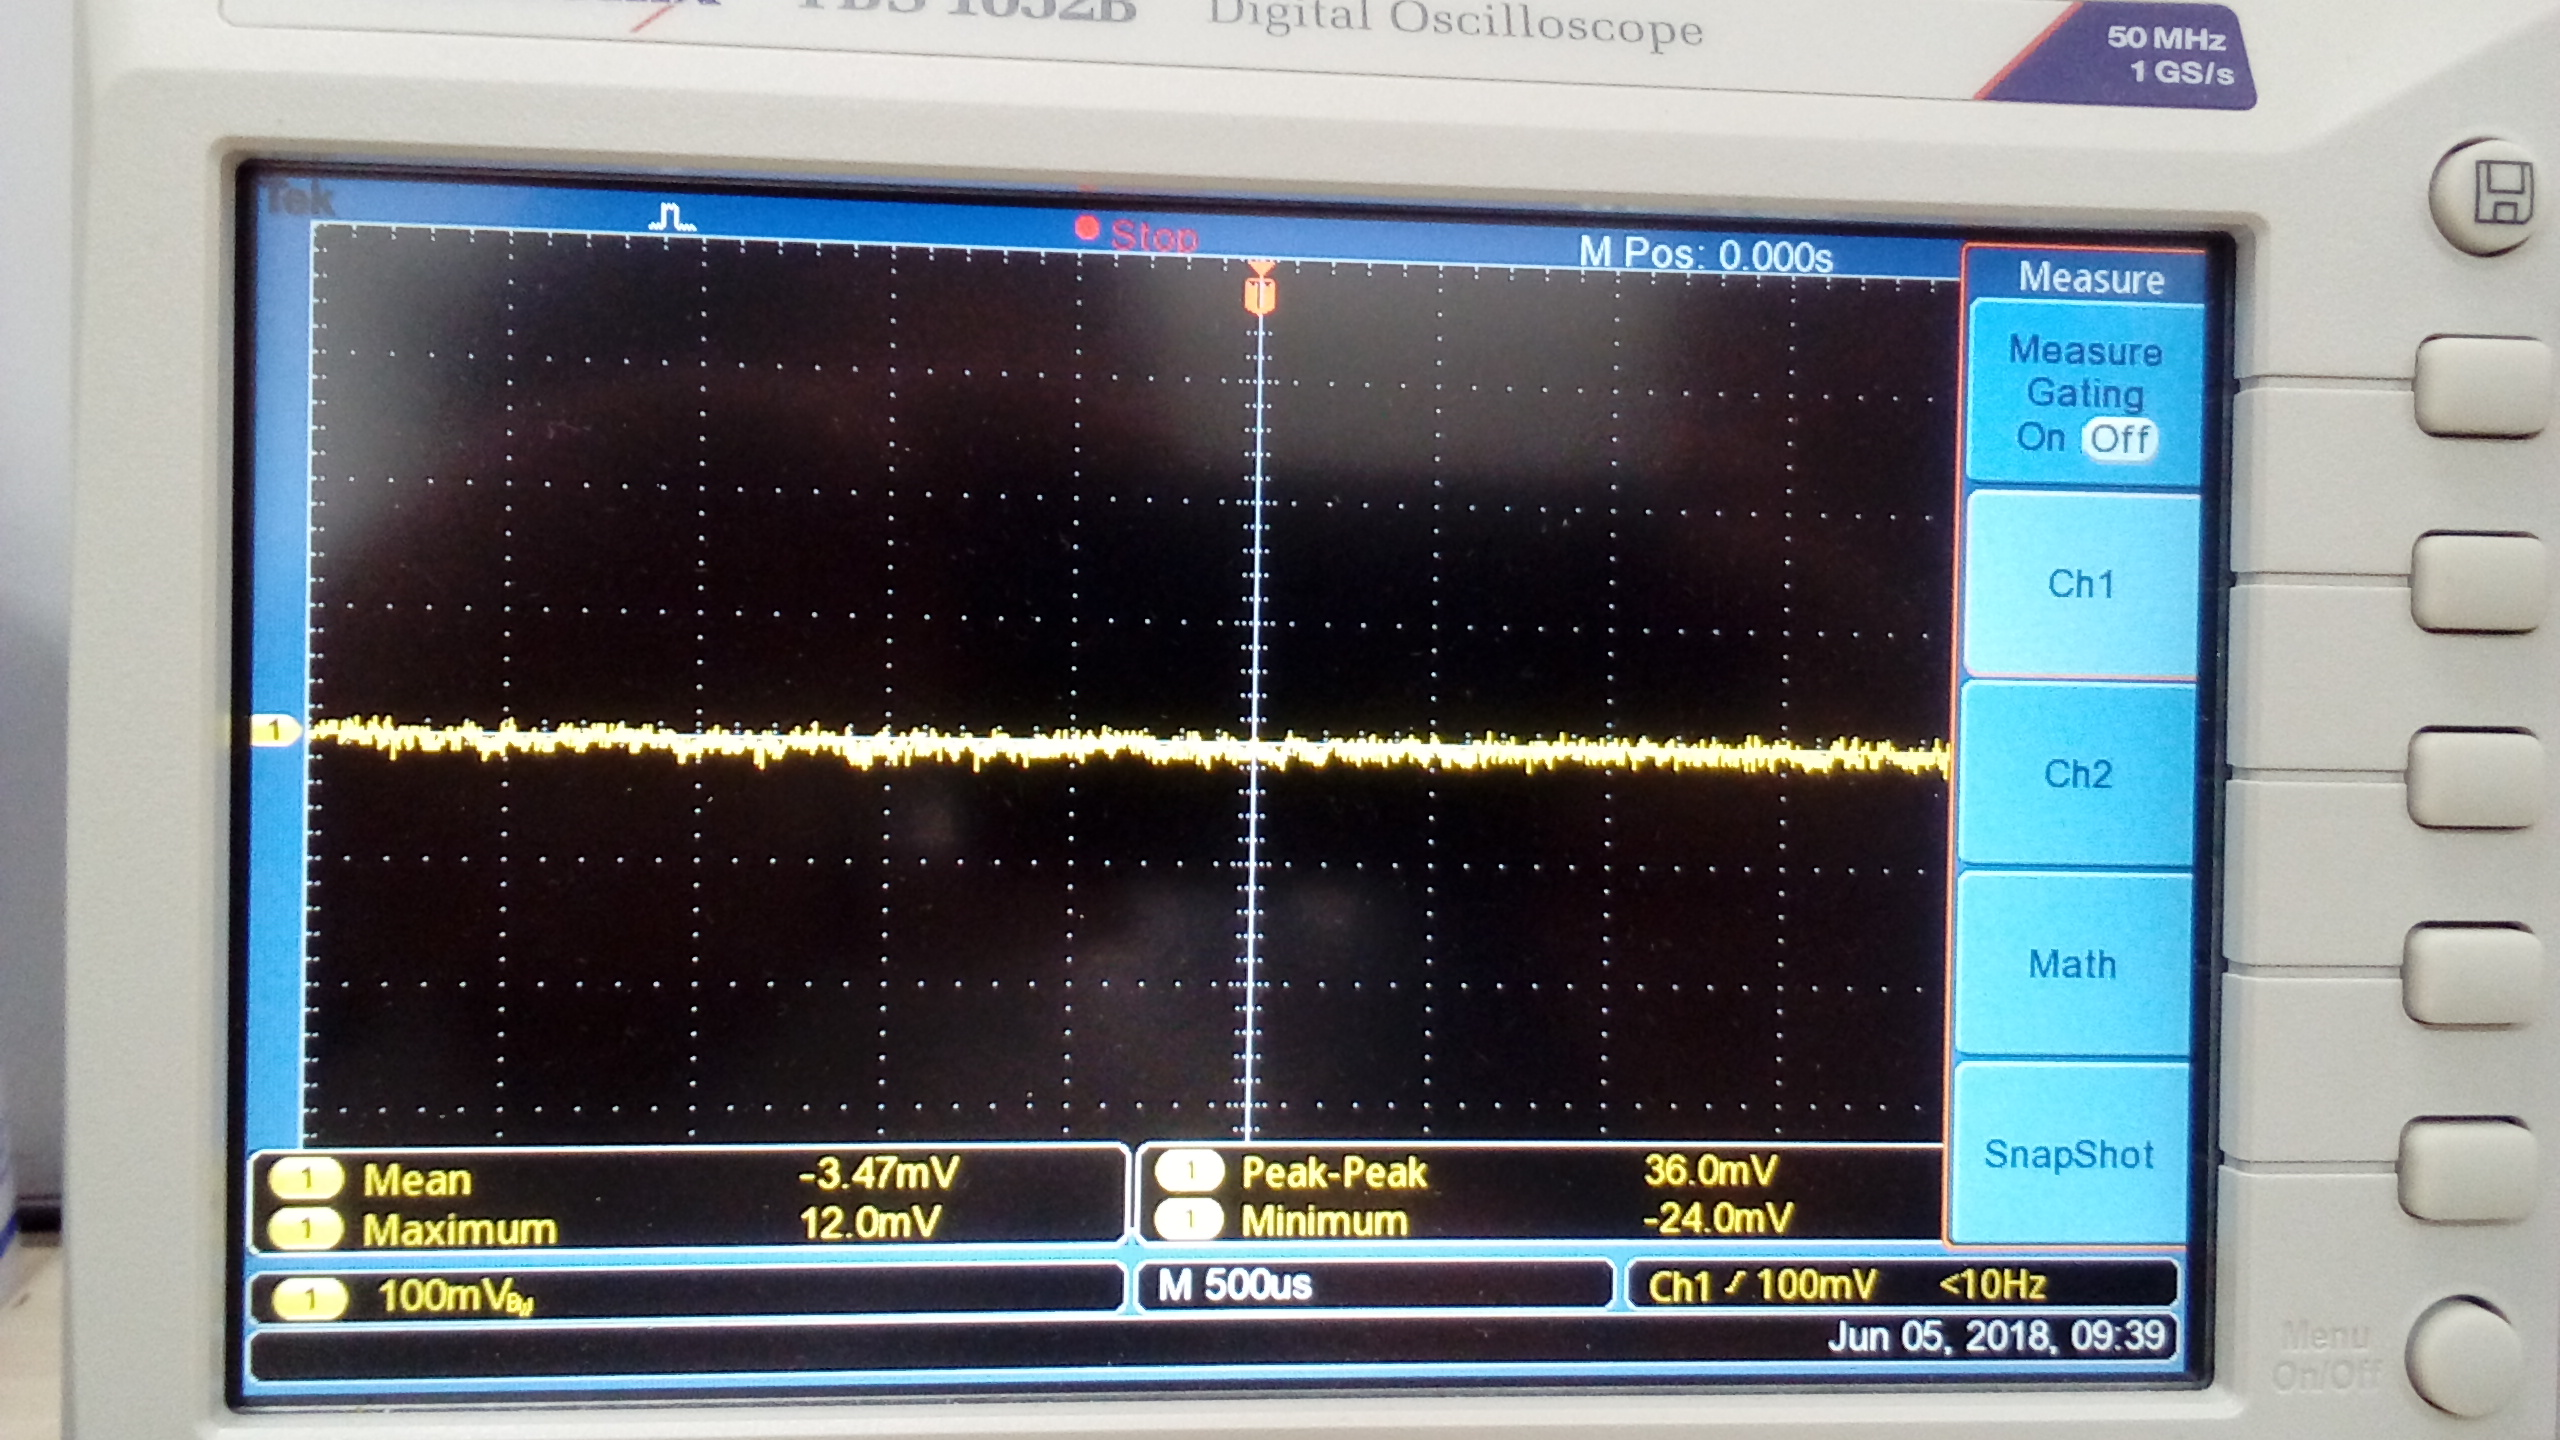
\includegraphics[width = \linewidth]{../Fotos/depoisFiltro33.jpg}
					\caption{Sinal AC da saída do filtro LC de 3,3V}
				\end{minipage}
			\end{figure}

			\begin{figure}[!ht]
				\centering
				\begin{minipage}{0.4\linewidth}
					\centering
					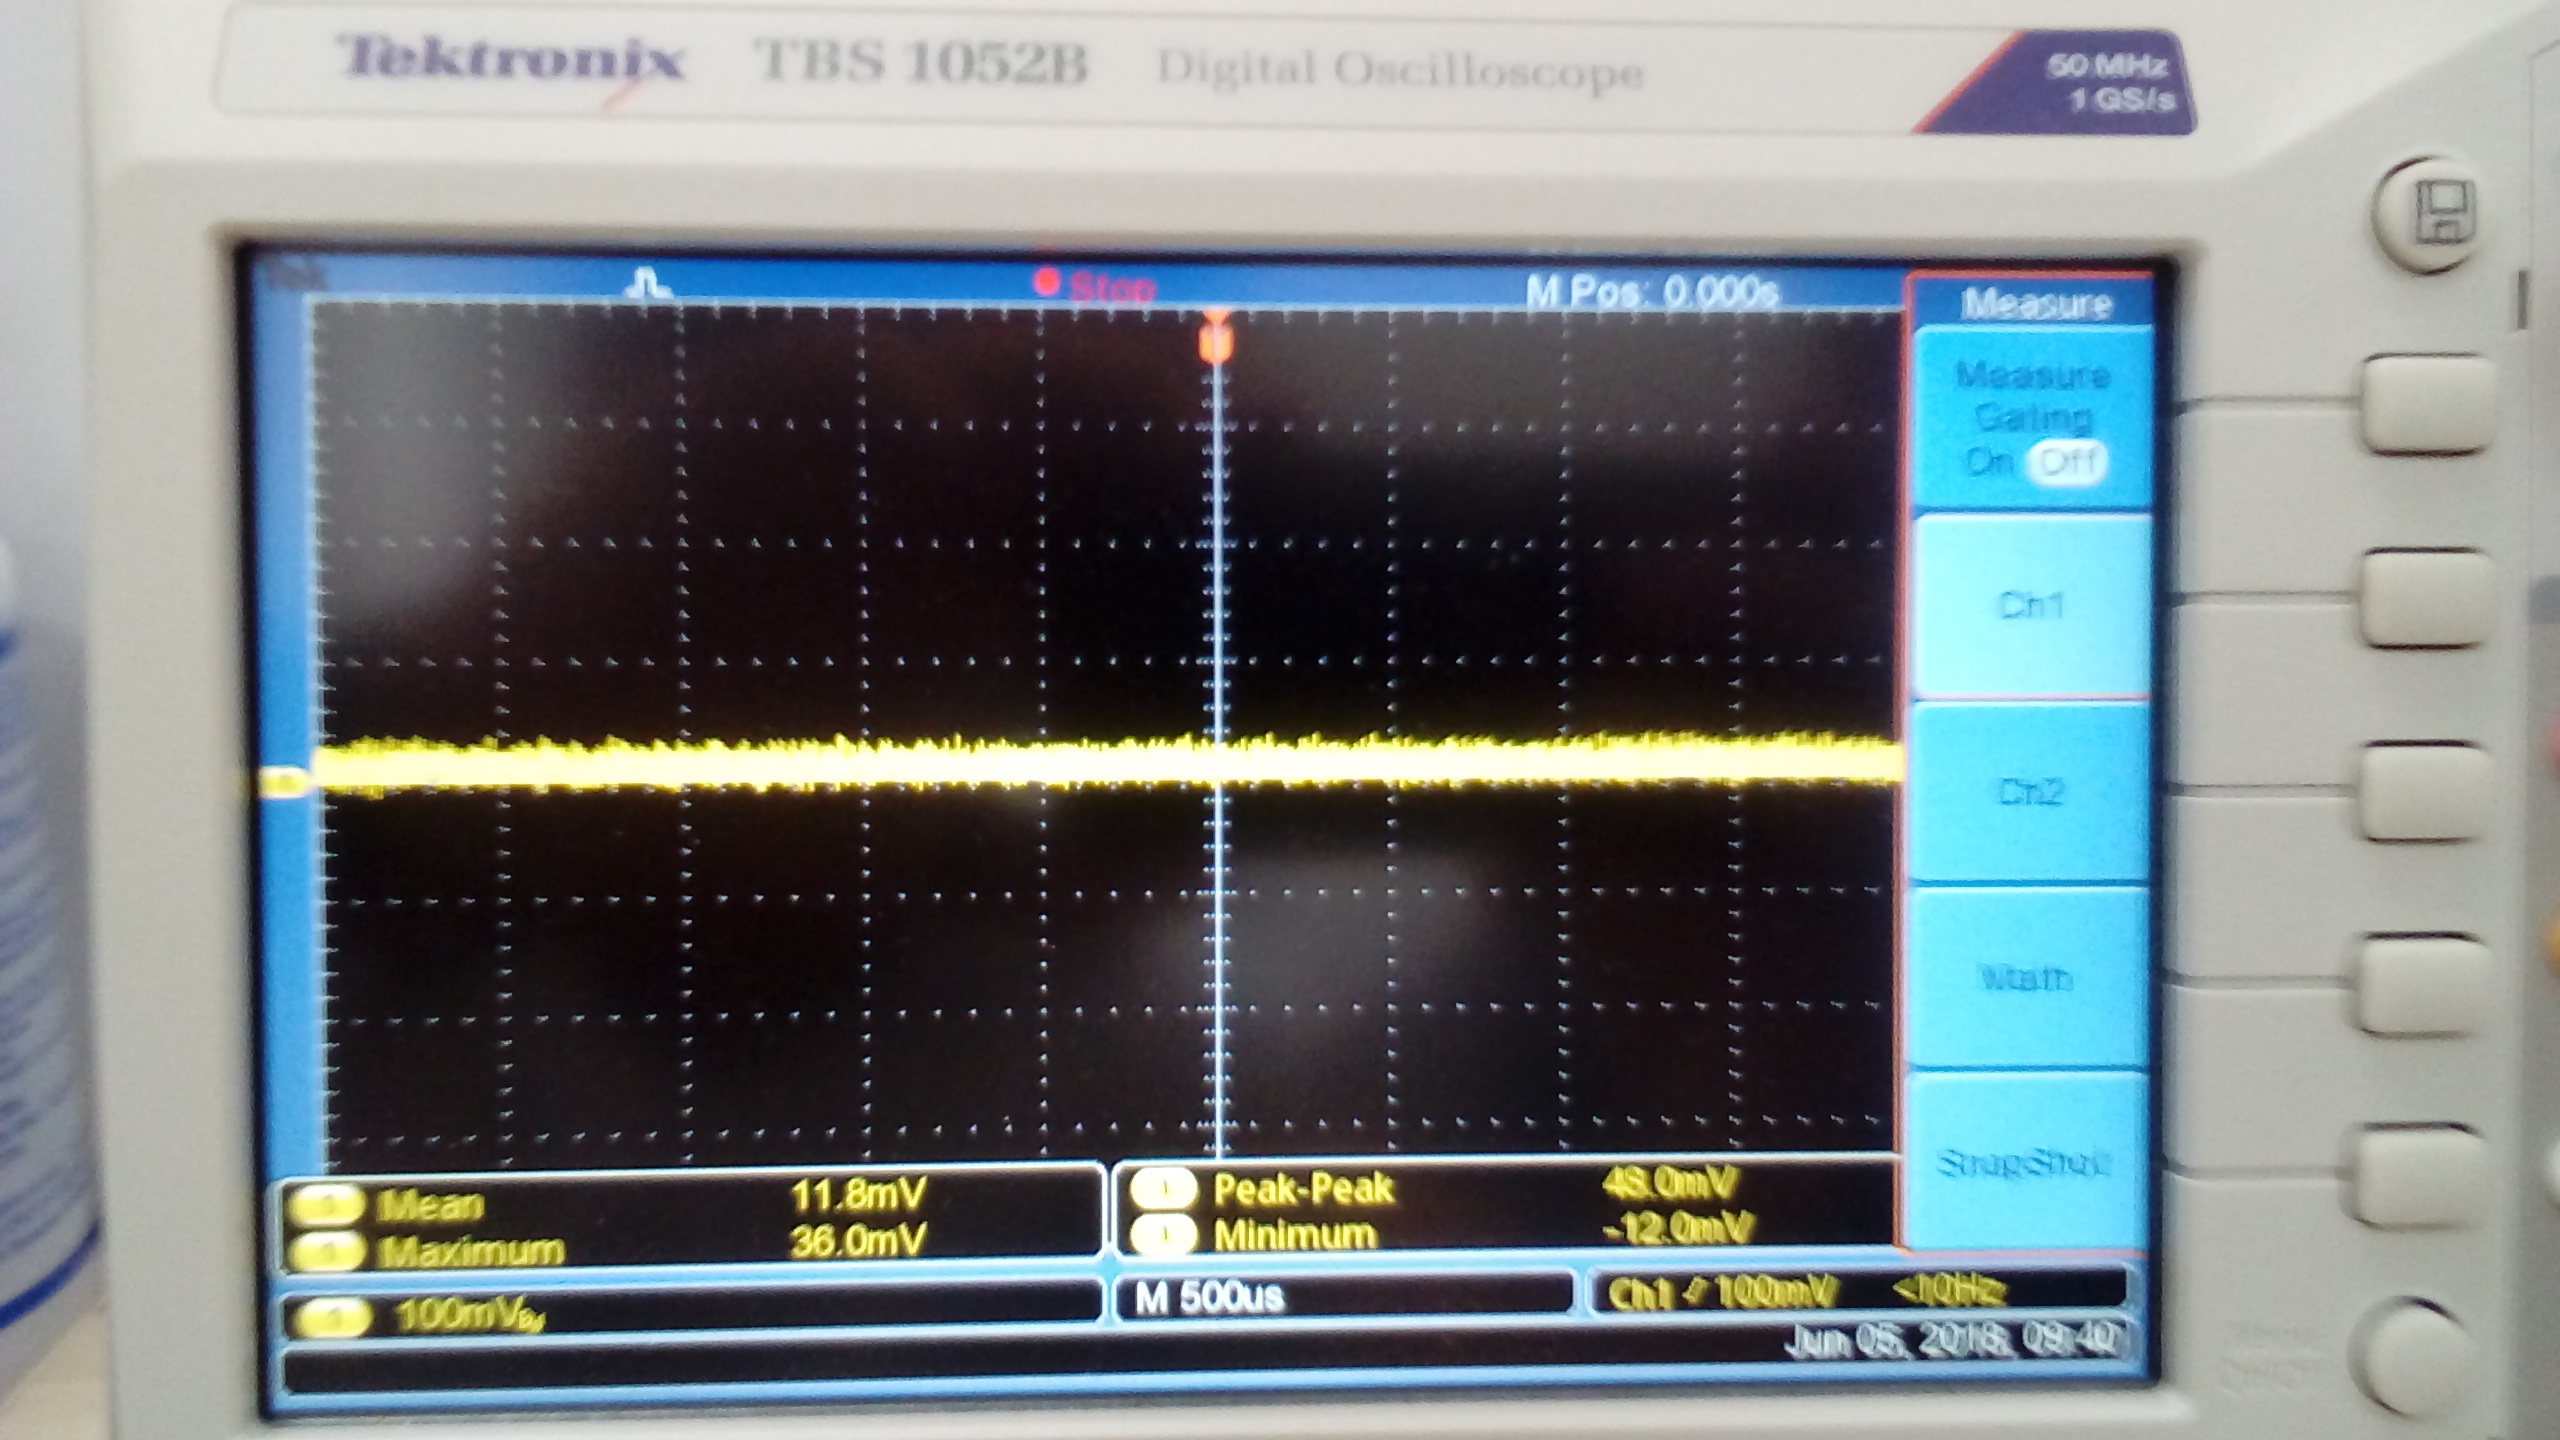
\includegraphics[width = \linewidth]{../Fotos/antesFiltro19.jpg}
					\caption{Sinal AC da saída da fonte de 19V}
				\end{minipage}
				\hfill\vline\hfill
				\begin{minipage}{0.4\linewidth}
					\centering
					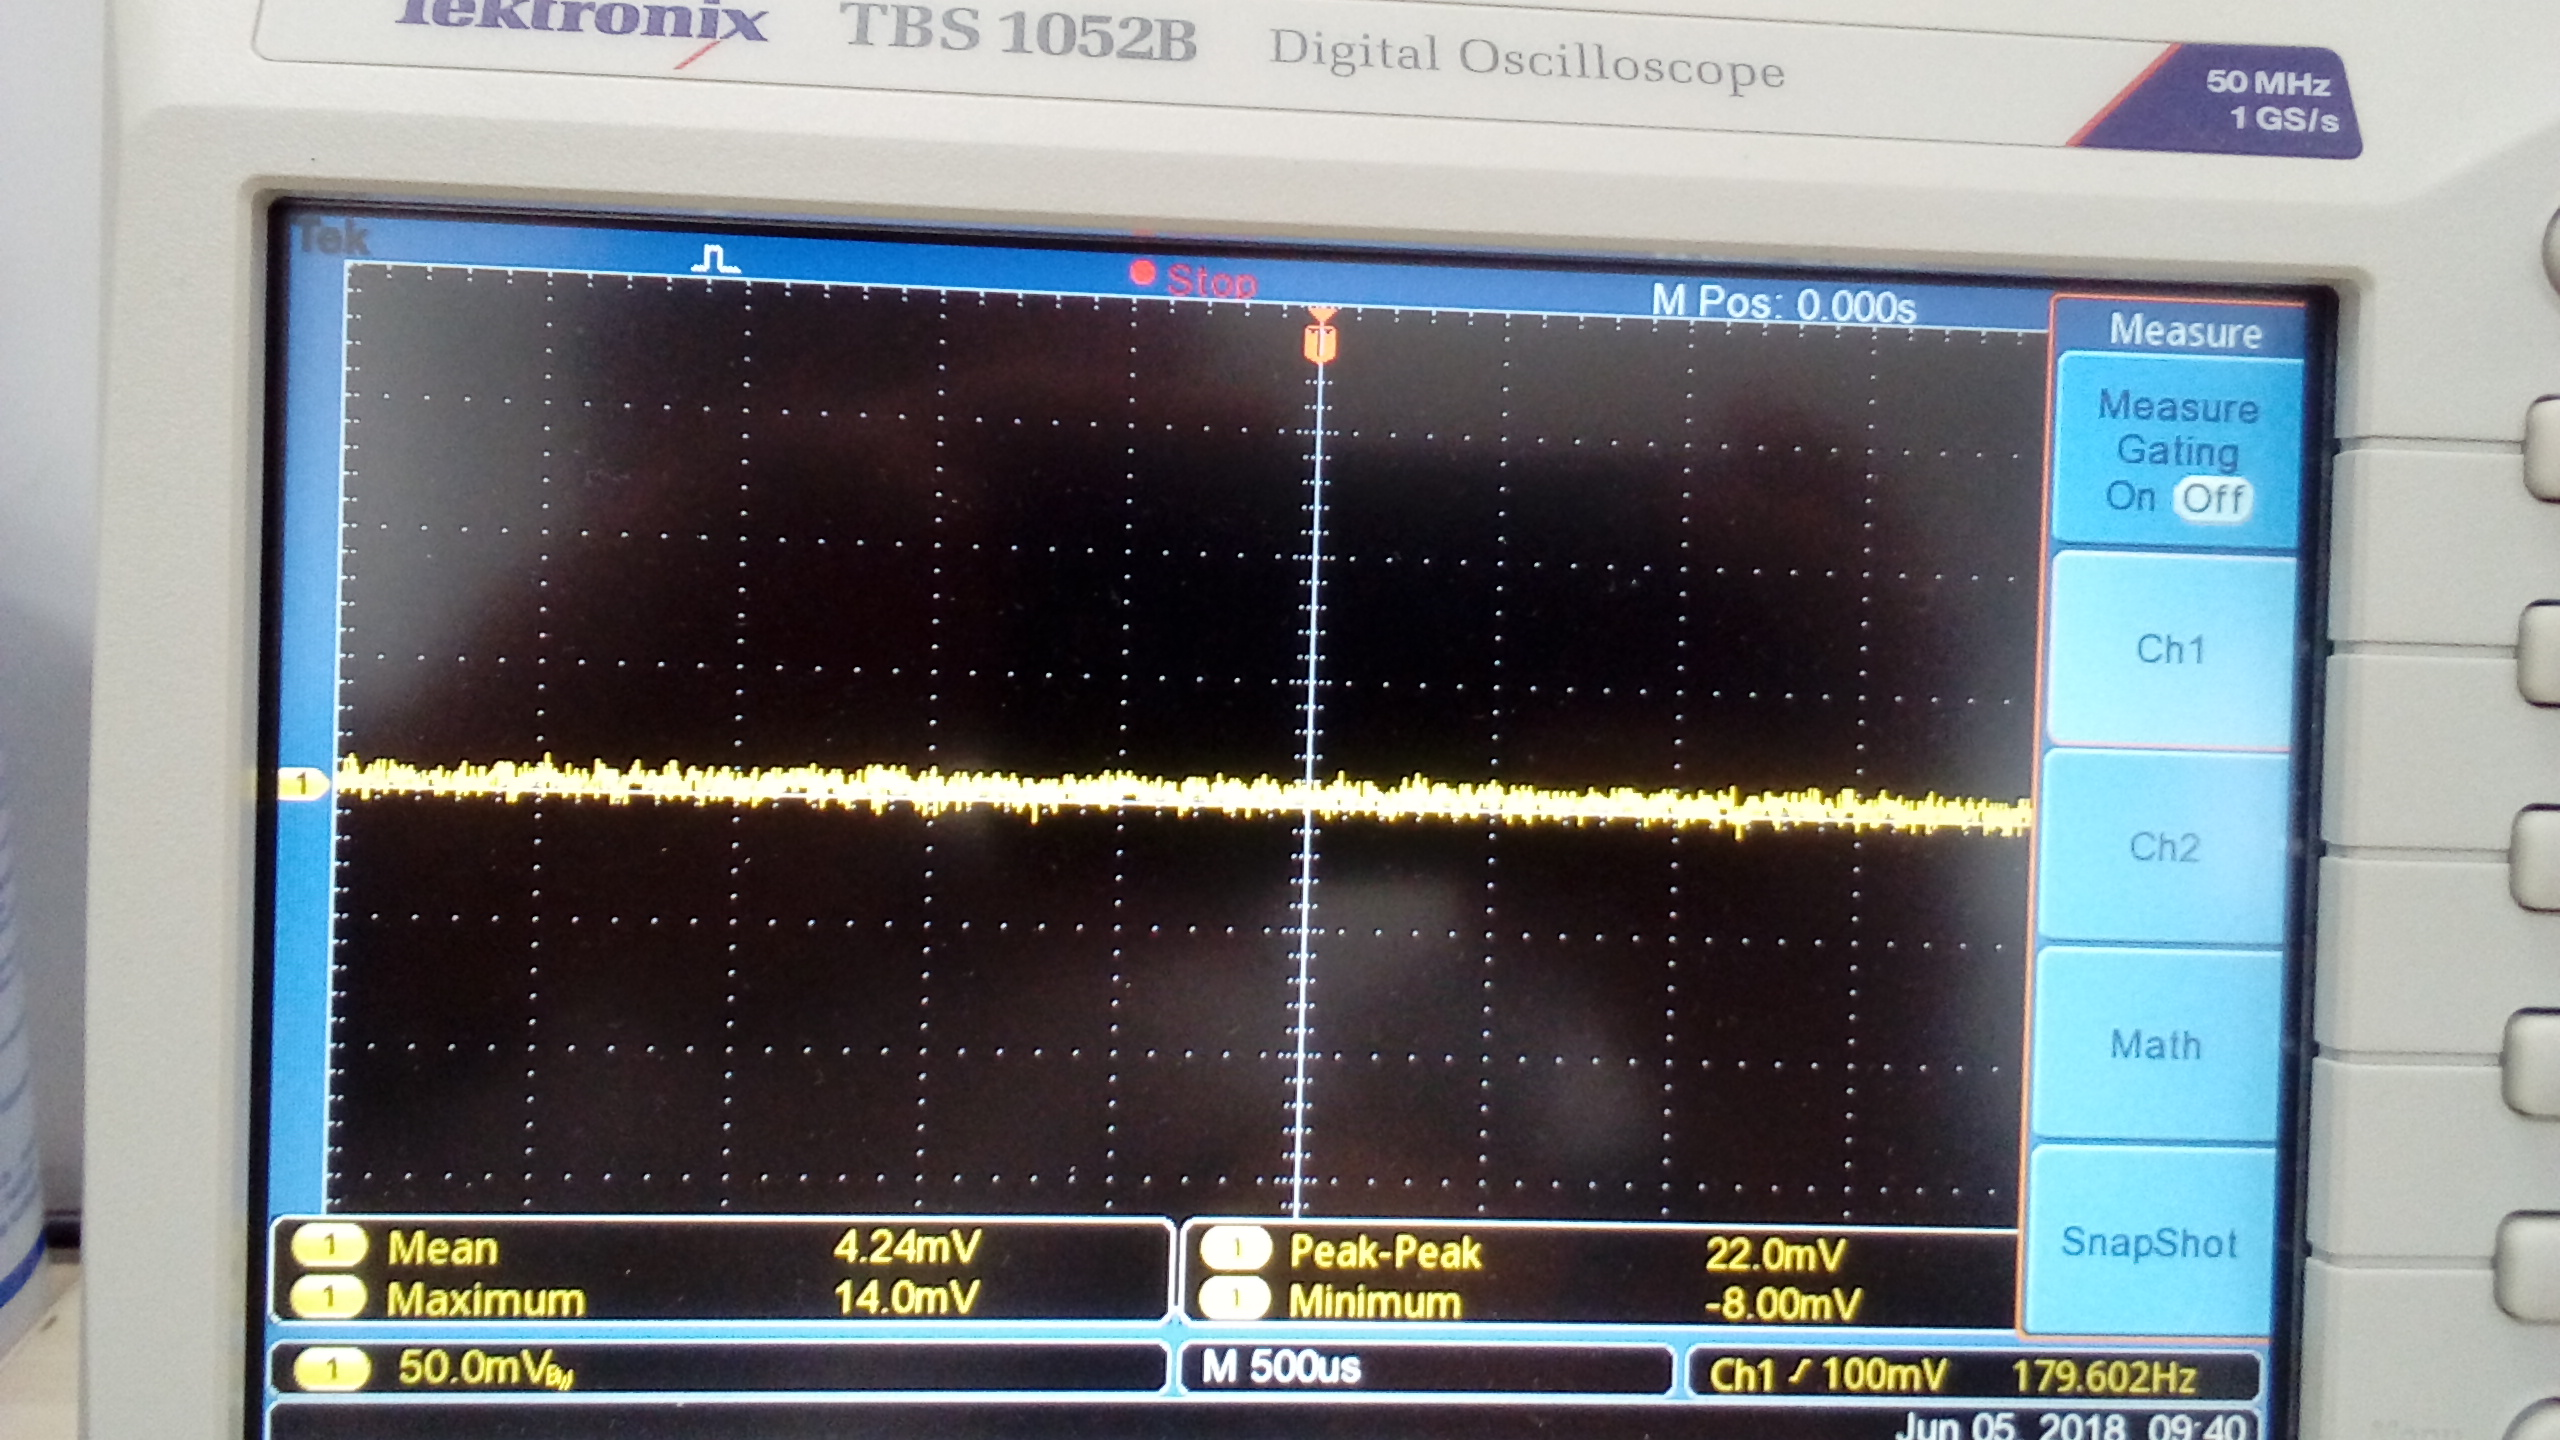
\includegraphics[width = \linewidth]{../Fotos/depoisFiltro19.jpg}
					\caption{Sinal AC da saída do filtro LC de 19V}
				\end{minipage}
			\end{figure}

			Os filtros chegaram a reduzir $73\%$ dos valores AC pico a
			pico da saída da fonte de tensão de $3,3V$. Porém, quando o
			módulo de telemetria operava no modo de envio era possível
			observar oscilações de alta frequência na alimentação, como
			mostrado na Figura ~\ref{fig:oscNrf}, chegando a picos positivos de $0,24V$
			e picos negativos de $0.28V$.
			
			\begin{figure}[!ht]
				\centering
				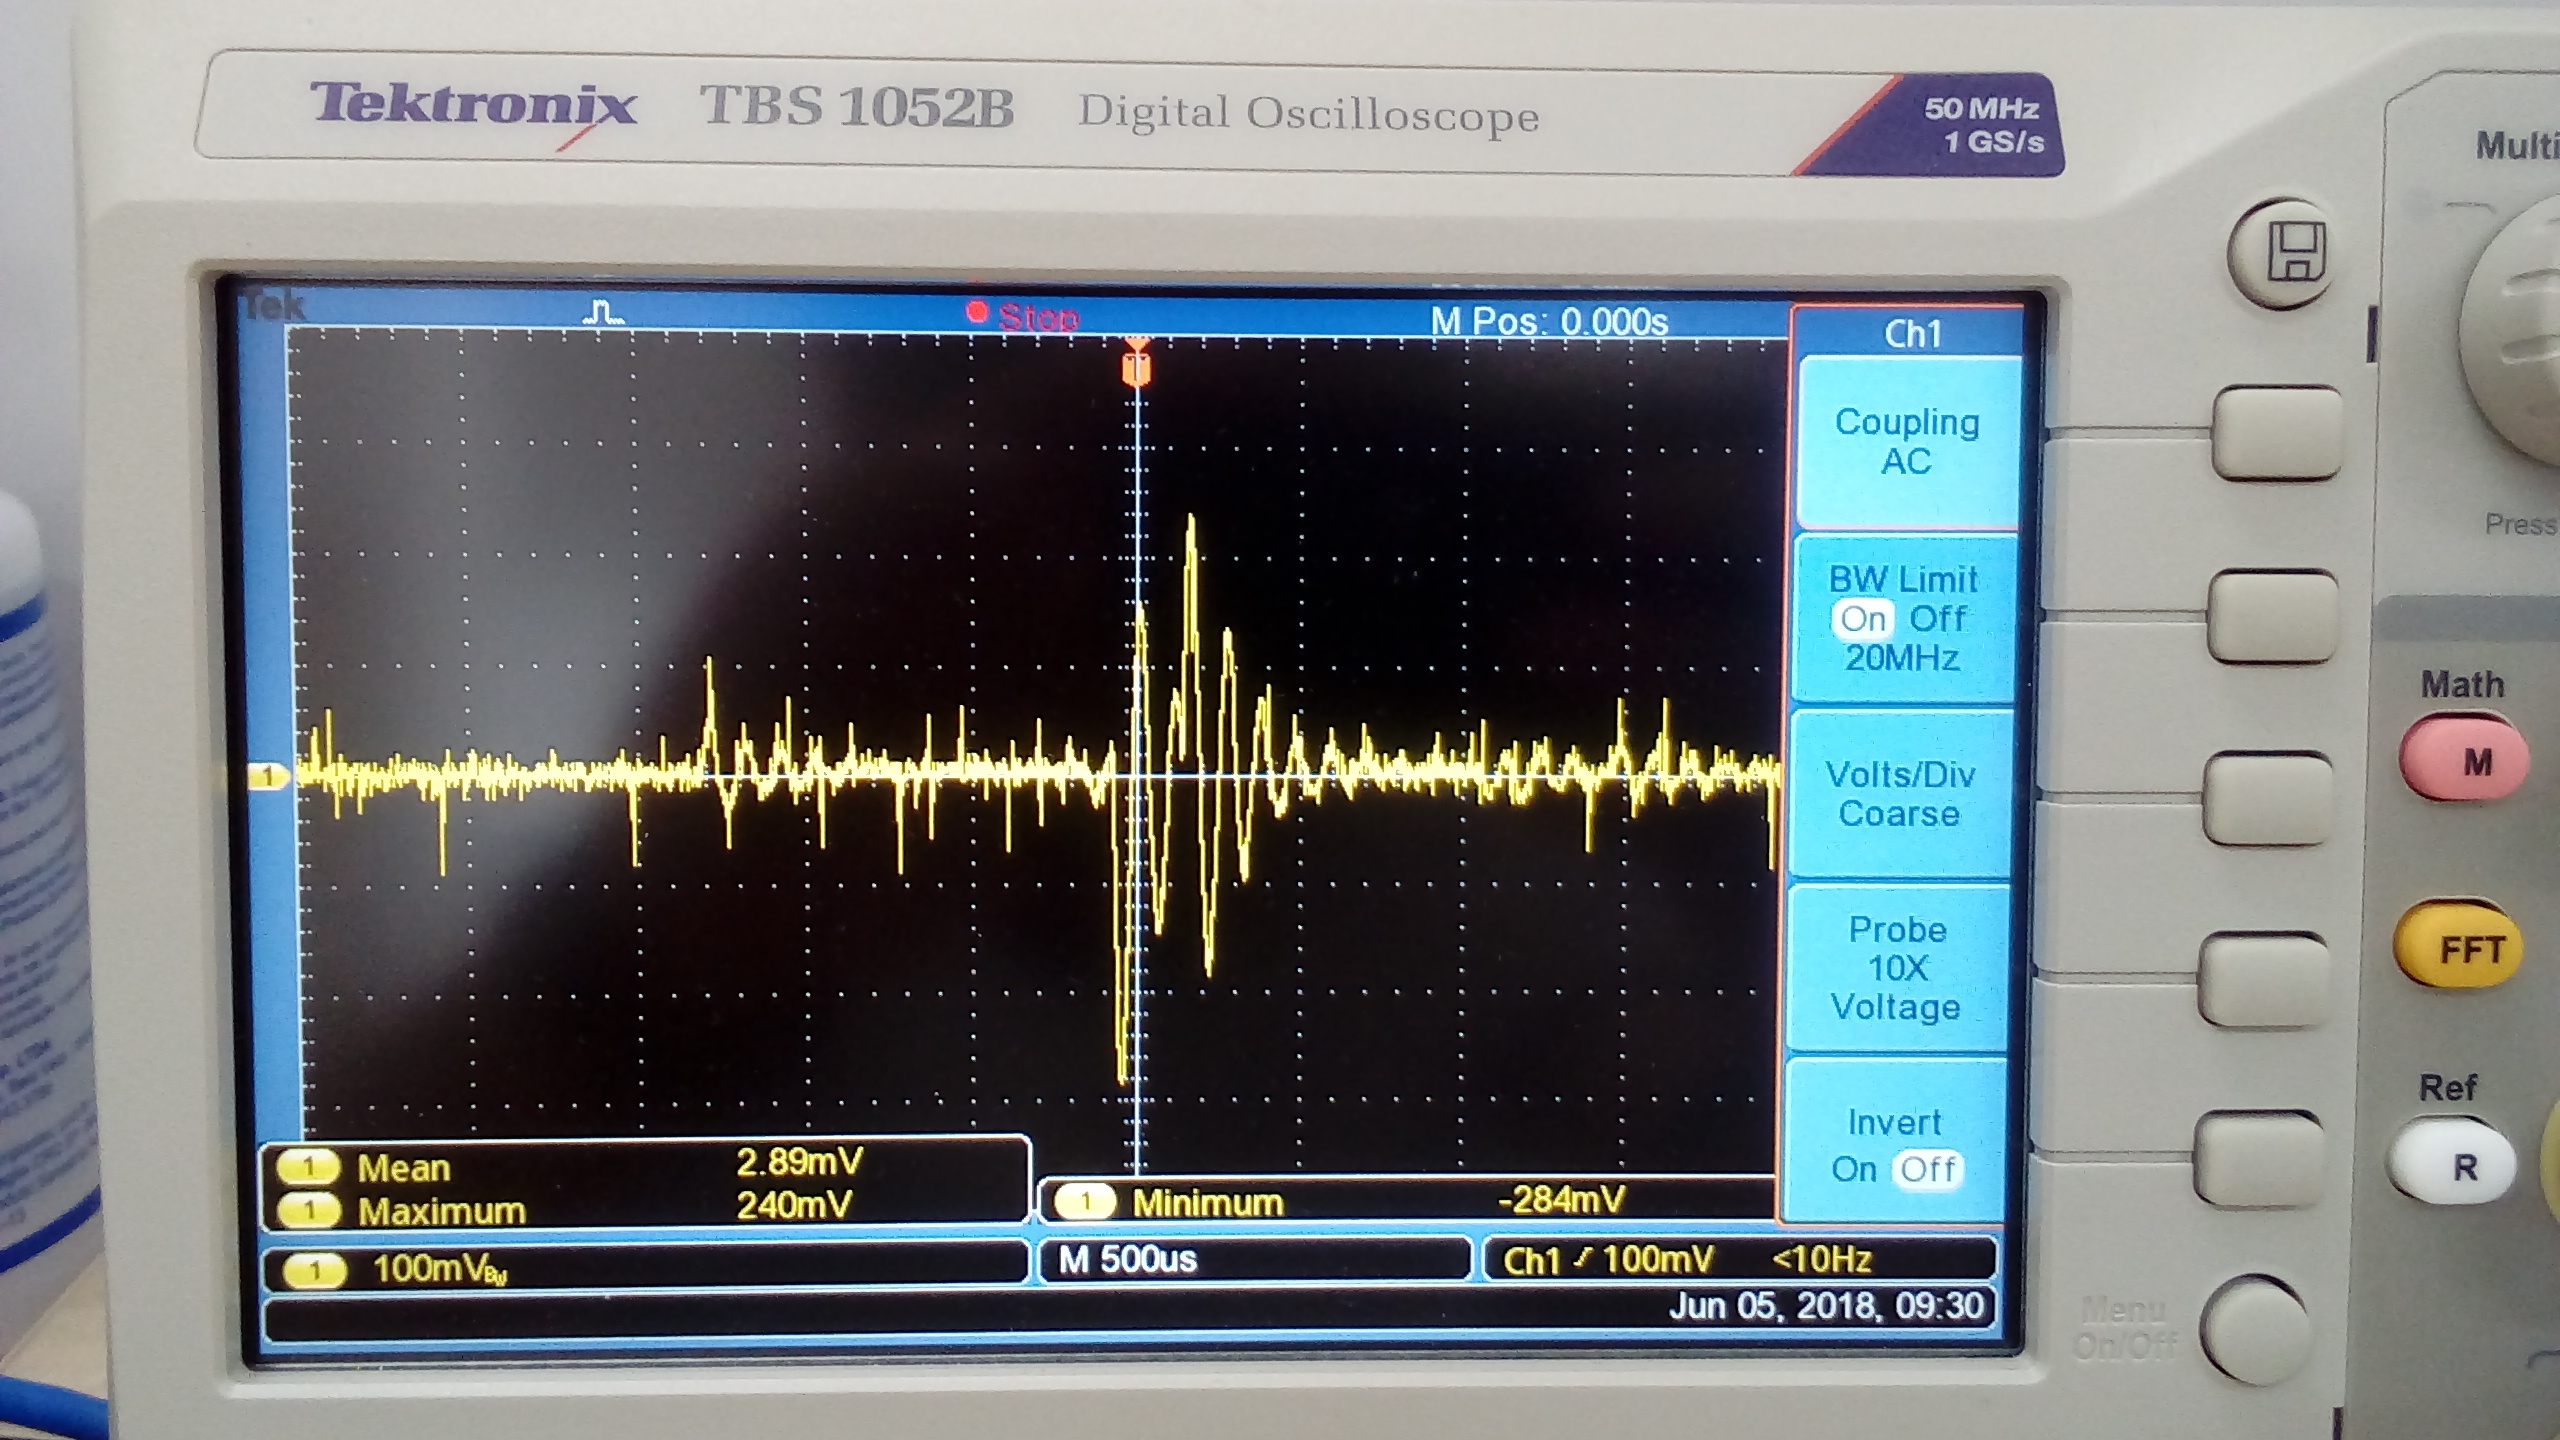
\includegraphics[width = \linewidth]{../Fotos/osc33.jpg}
				\caption{Oscilações causadas pelo modo de telemetria}
				\label{fig:oscNrf}
			\end{figure}

		\subsection{Condicionamento de sinal}
			Conectou-se um acelerômetro à entrada BNC e mediu-se a
			tensão do sinal quando em uma superfície sem vibração e
			obteve-se um valor médio de $11,76V$. A tensão medida após o
			condicionamento do sinal foi de 1,992V. Assim, o ganho $G$
			medido foi de $G = 0,1694V/V$, próximo do valor calculado de $0,1737V/V$ na seção 3.3 desta monografia. Assim, consegue-se atenuar o sinal para níveis de tensão dentro da faixa de medição do ADC.

			\begin{figure}[!ht]
				\centering
				\begin{minipage}{0.4\linewidth}
					\centering
					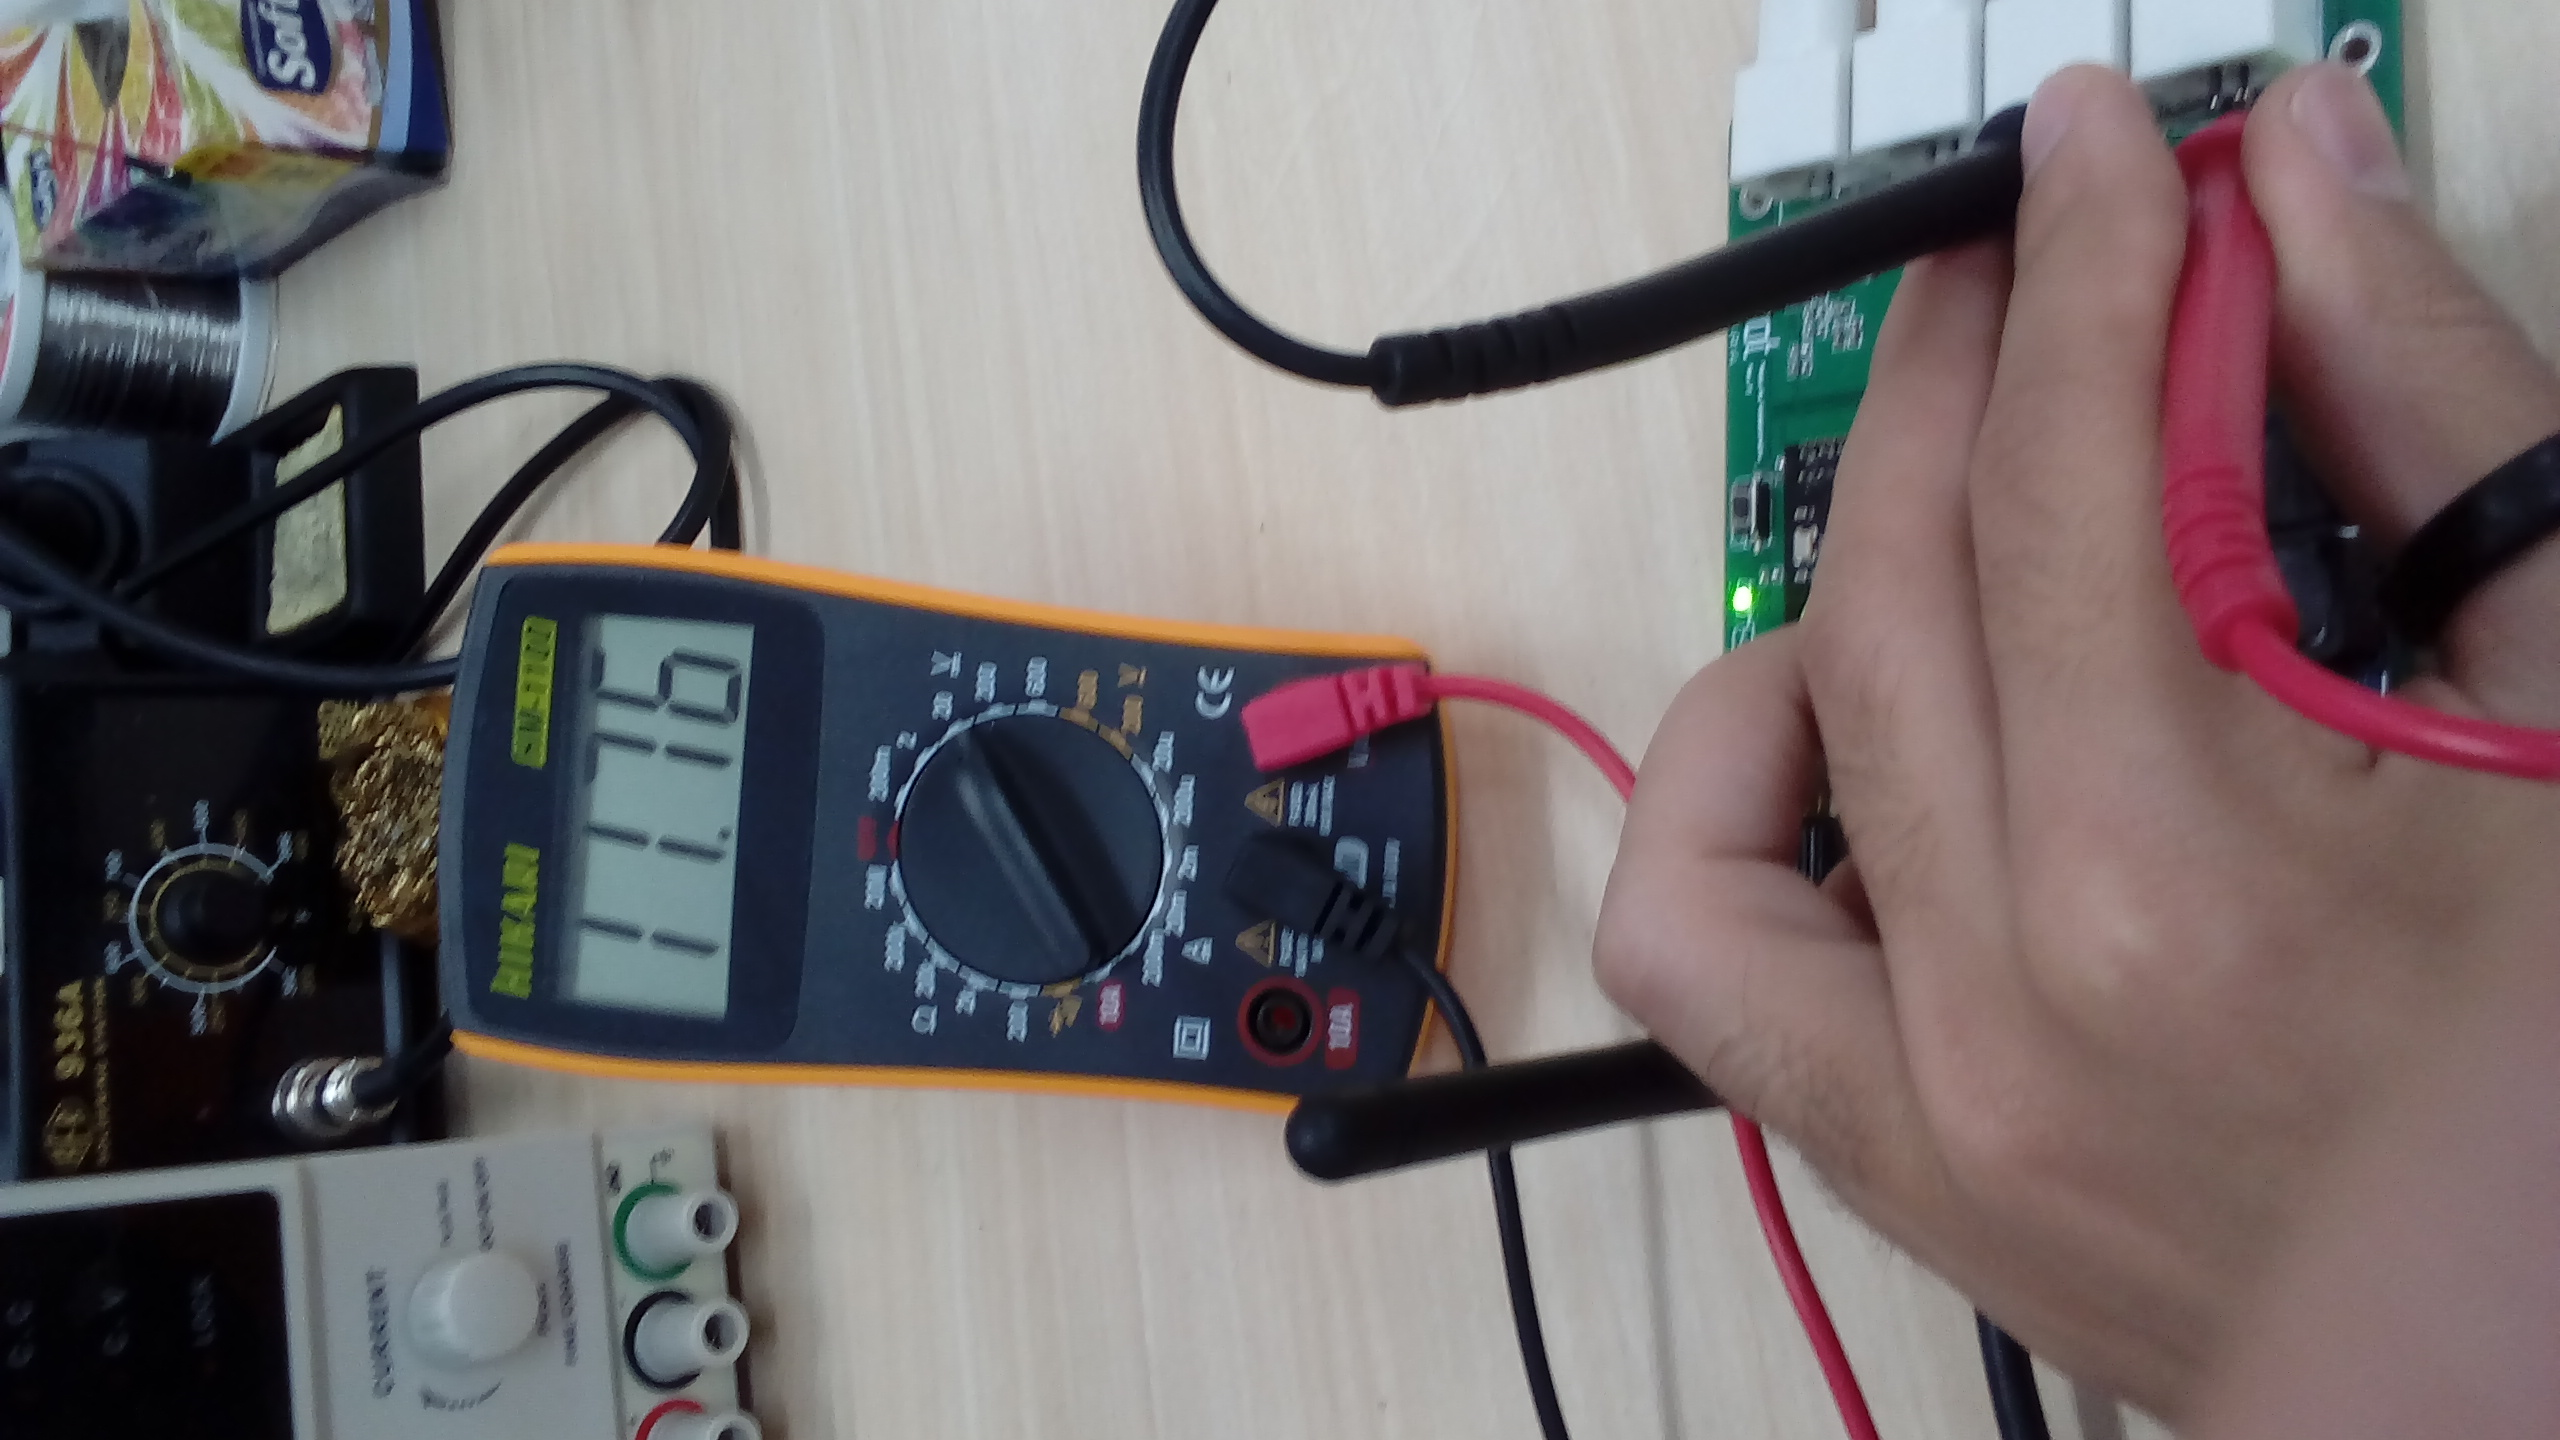
\includegraphics[angle=-90,width = \linewidth]{../Fotos/tensaoAcc.jpg}
					\caption{Tensão média do acelerômetro}
				\end{minipage}
				\hfill\vline\hfill
				\begin{minipage}{0.4\linewidth}
					\centering
					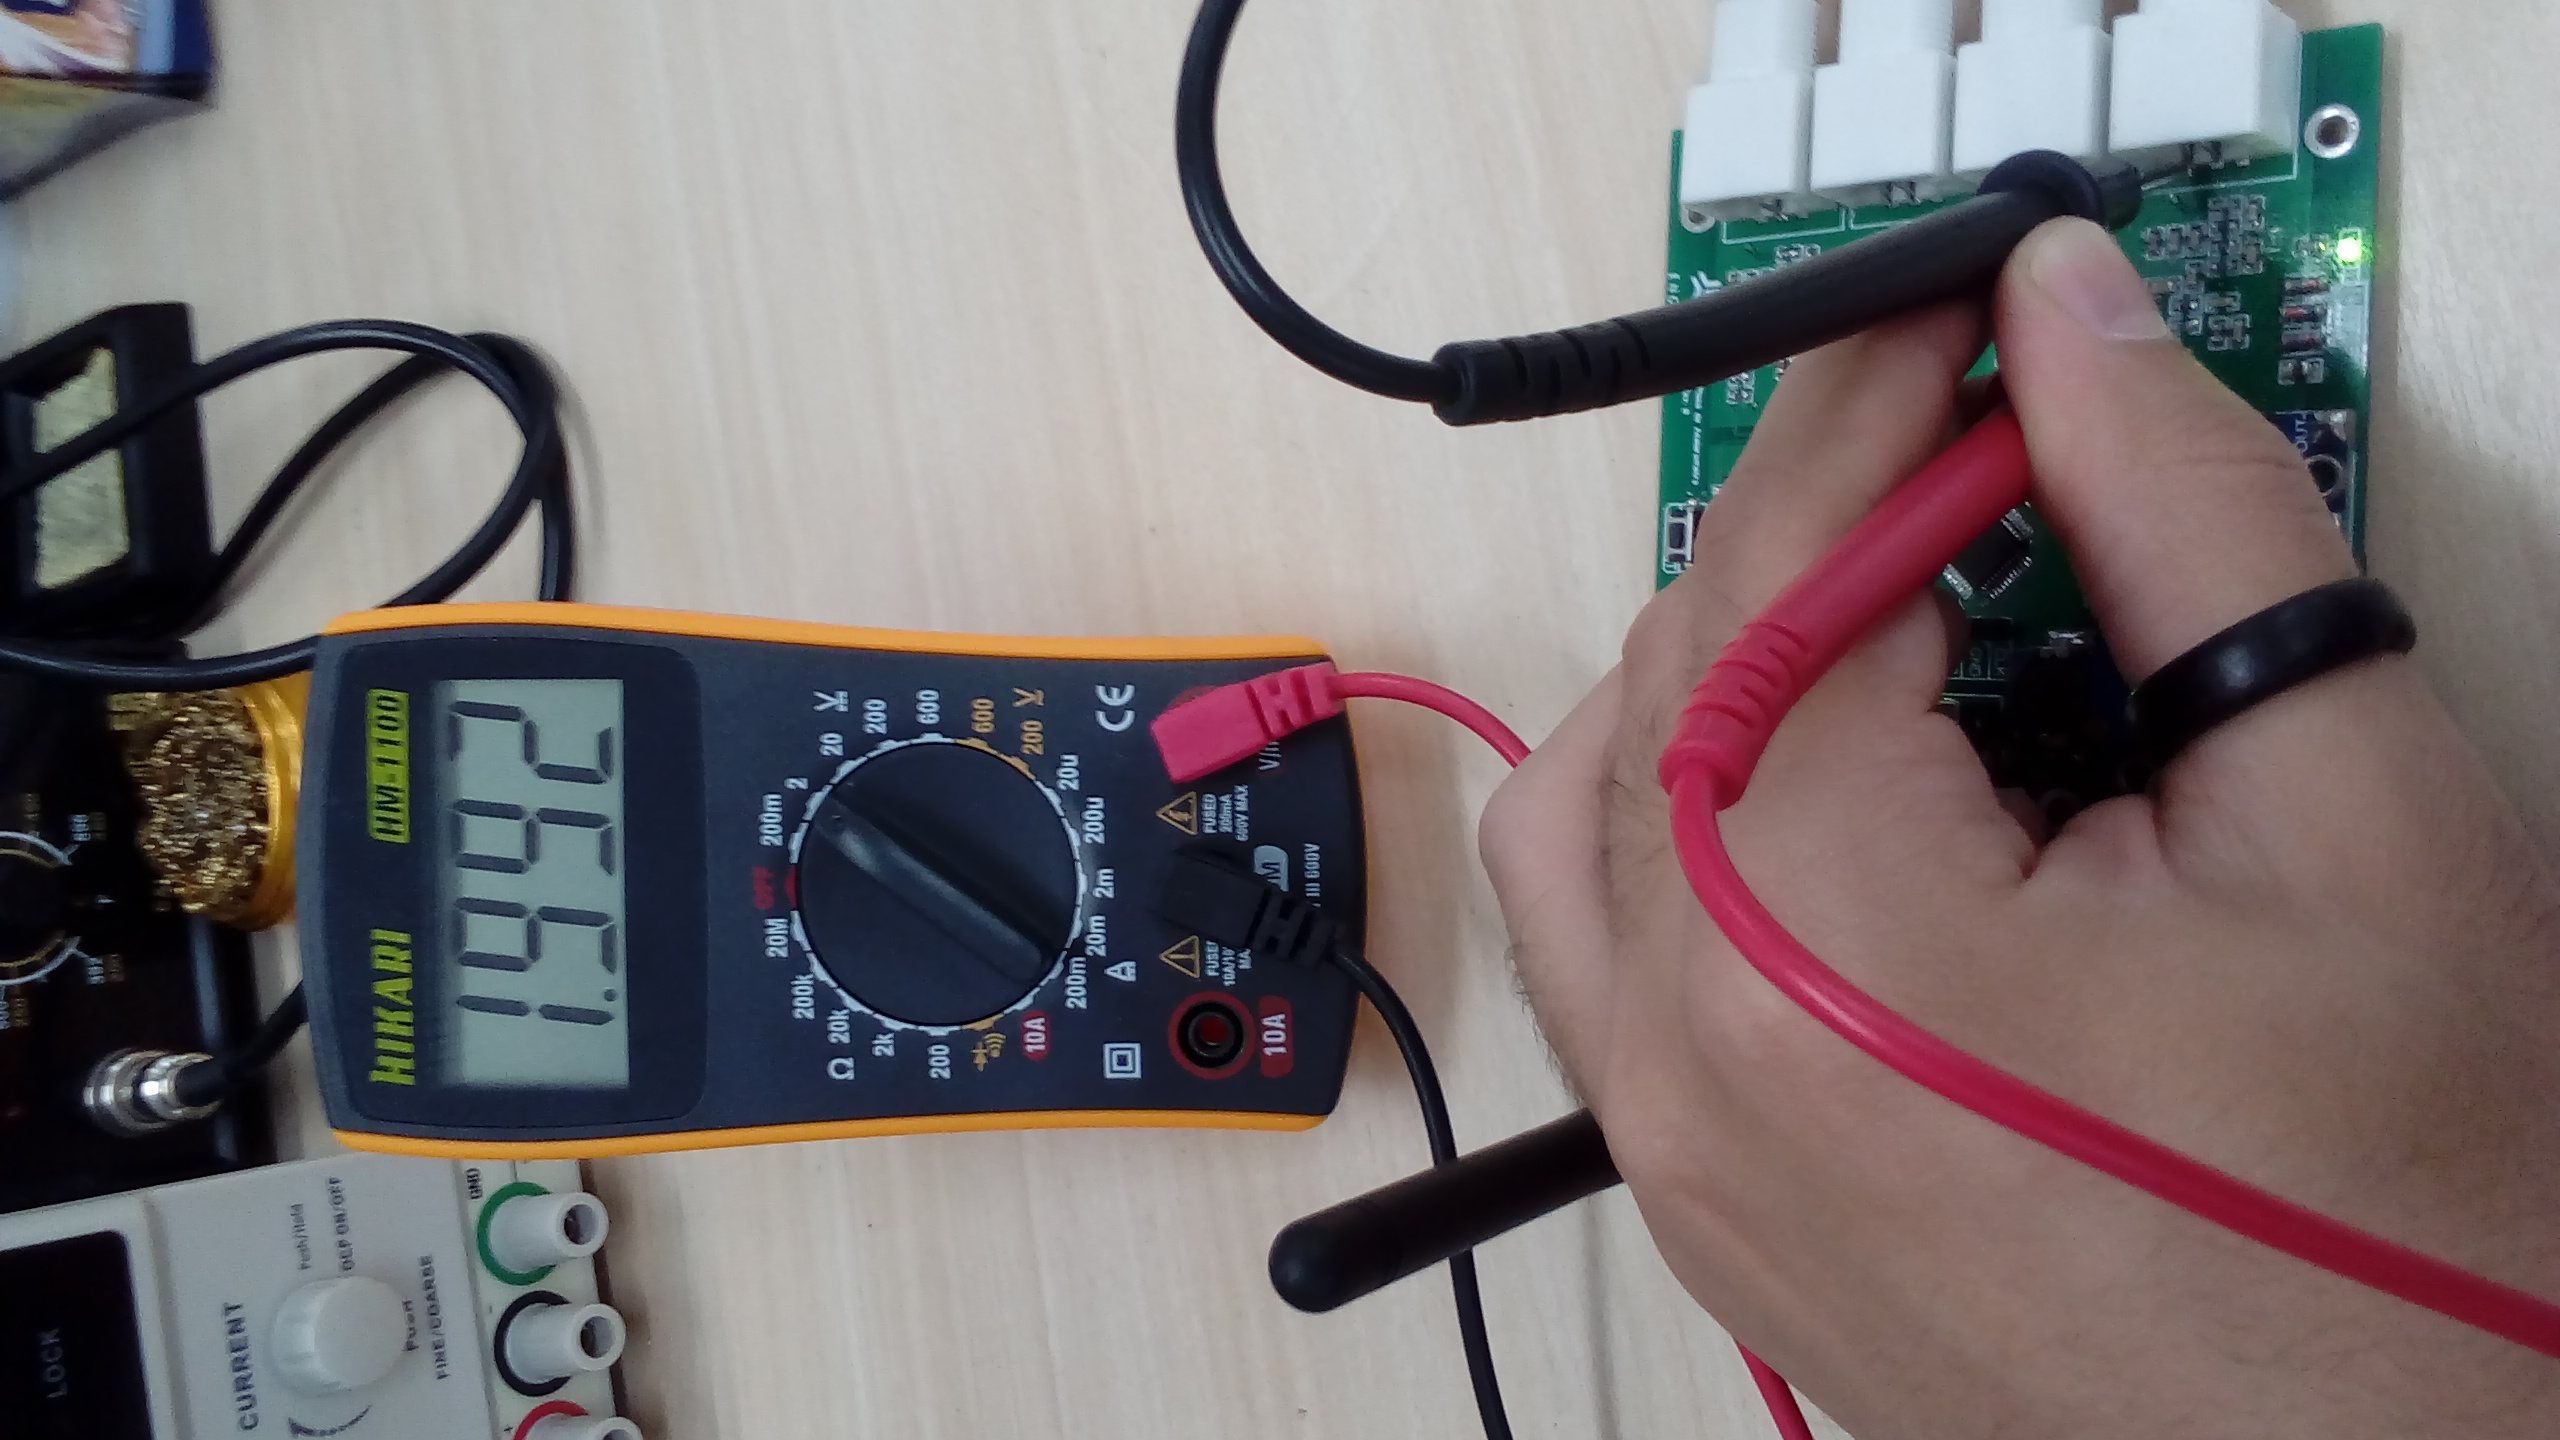
\includegraphics[angle=-90,width = \linewidth]{../Fotos/tensaoAccG.jpg}
					\caption{Tensão média do acelerômetro após o ganho}
				\end{minipage}
			\end{figure}

			Ao utilizar um outro acelerômetro de mesmo modelo, os
			valores de tensão média variaram, chegando a $13,8V$. Assim,
			é necessário um ajuste de \textit{offset} em toda rotina de
			início de amostragem.

			\newpage

	\section{Consumo}
		Para realizar a programação, utilizou-se o programador
		ST-LINK/V2, conectado à placa como apresentado na Figura ~\ref{fig:accConectados}. Para
		o recebimento dos dados, um outro módulo recebia os dados e
		os transmitia por USB via terminal serial.

		\begin{figure}[!ht]
			\centering
			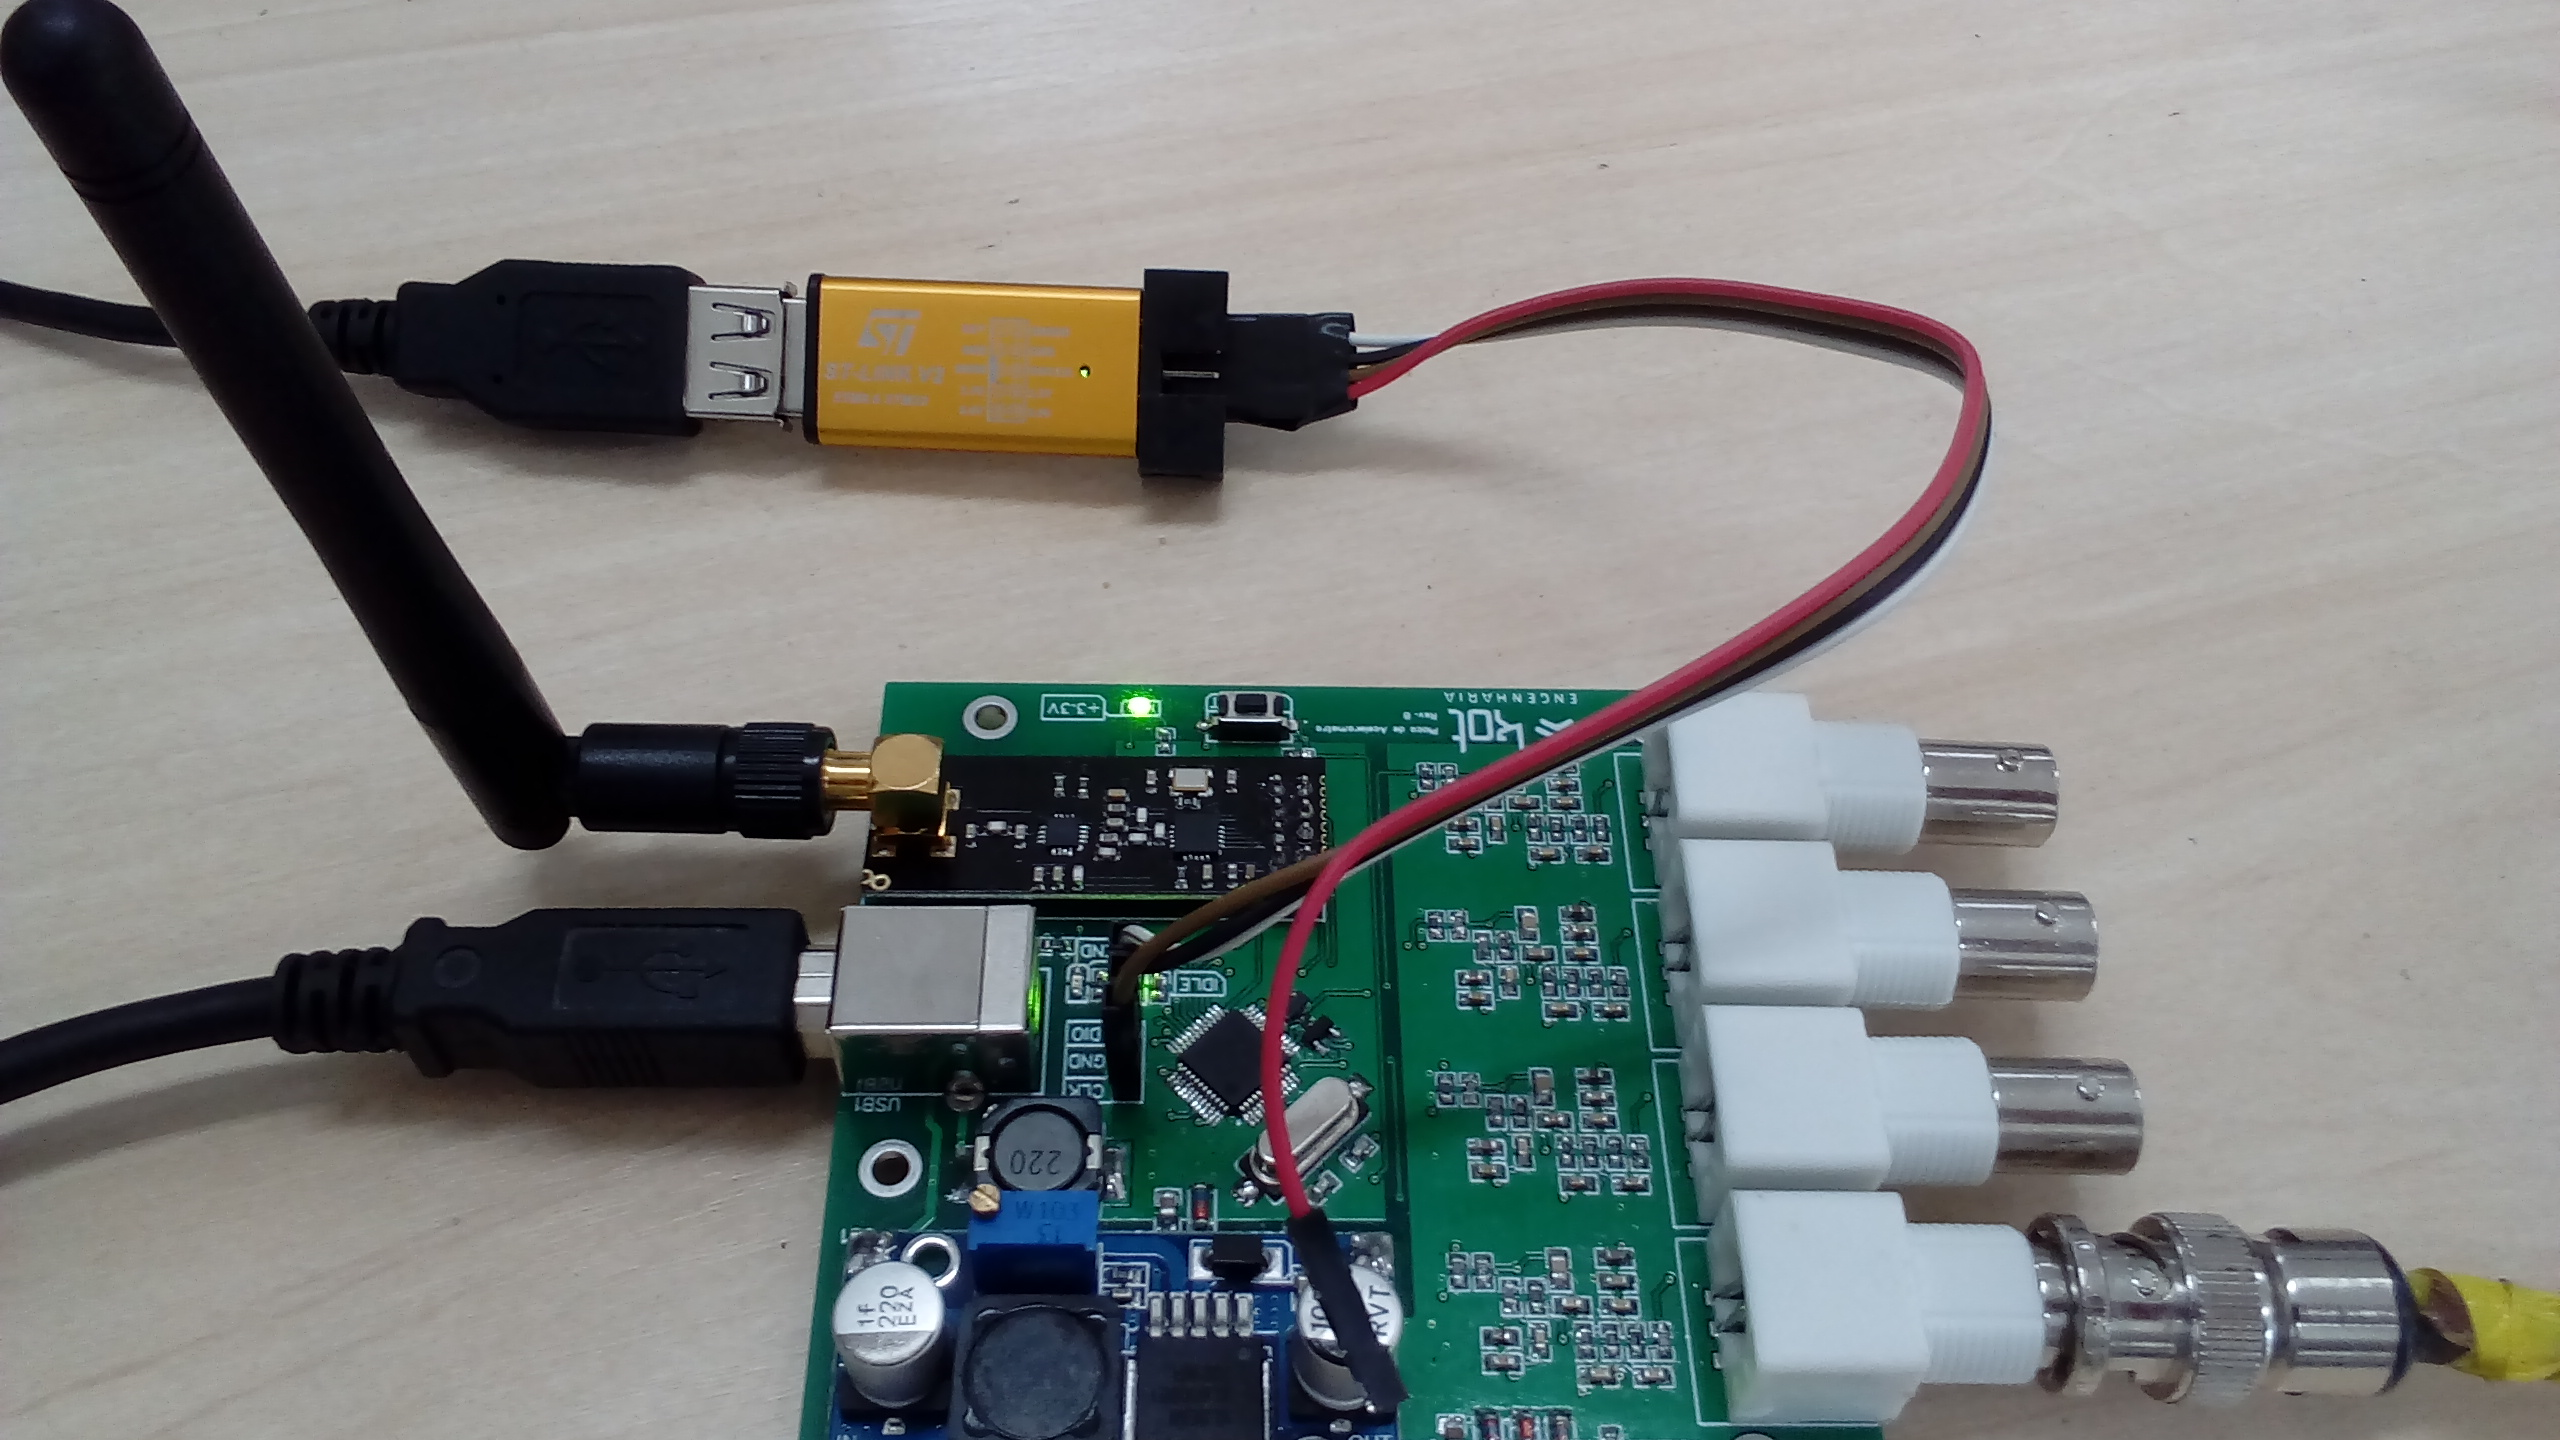
\includegraphics[width=\linewidth]{../Fotos/stlink.jpg}
			\caption{Placa sem acelerômetros conectados, em modo \textit{standby}}
			\label{fig:accConectados}
		\end{figure}

		Utilizando a fonte Hikari HF-3203S, alimentou-se a fonte com $5V$
		regulados e analisou o desempenho traduzido no consumo de
		corrente do circuito em diferentes condições de operação.

		Pôde-se notar um aumento de aproximadamente $15$ a $20mA$ no consumo
		de corrente por canal, não ultrapassando $270mA$. A potência da
		placa ficou maior que a estimada, com $1,35W$. Isso ocorreu devido
		a presença dos LEDs que foram utilizados para indicar quando a
		placa está ligada e enviando. Porém, apenas um LED se faz
		necessário, reduzindo em torno de $30mA$ o consumo, fazendo com
		que a potência caia para $1,2W$, próximo aos $1,19W$ estimados.

		\newpage

	\section{Ensaios}
		Dois ensaios foram realizados. O primeiro ensaio consiste em utilizar um acelerômetro com base magnética posicionado na parte superior da peneira, como apresentado na Figura ~\ref{fig:accNaVertical}. O segundo ensaio também consiste em posicionar um acelerômetro com base magnética na peneira, porém na parte lateral, como apresentado na Figura ~\ref{fig:accNaLateral}, obtendo valores mais baixos de aceleração e frequência. O objetivo dos ensaios é avaliar a medição de sinais diferentes tanto em frequência quanto em amplitude, a fim de validar a linearidade da medição ao longo de parte da escala.
		
		Em um primeiro momento, o sinal foi aquisitado pelo sistema de aquisição NI	cDAQ-9178 em conjunto com o NI-9234, cedidos pela empresa supervisora, apresentados na Figura ~\ref{fig:modulosNI}. Acionou-se a peneira em $50\%$ de sua potência máxima. Coletou-se os dados para o acelerômetro na vertical e na lateral por 10 segundos cada.

		\begin{figure}[!ht]
			\centering
			\begin{minipage}{0.4\linewidth}
				\centering
				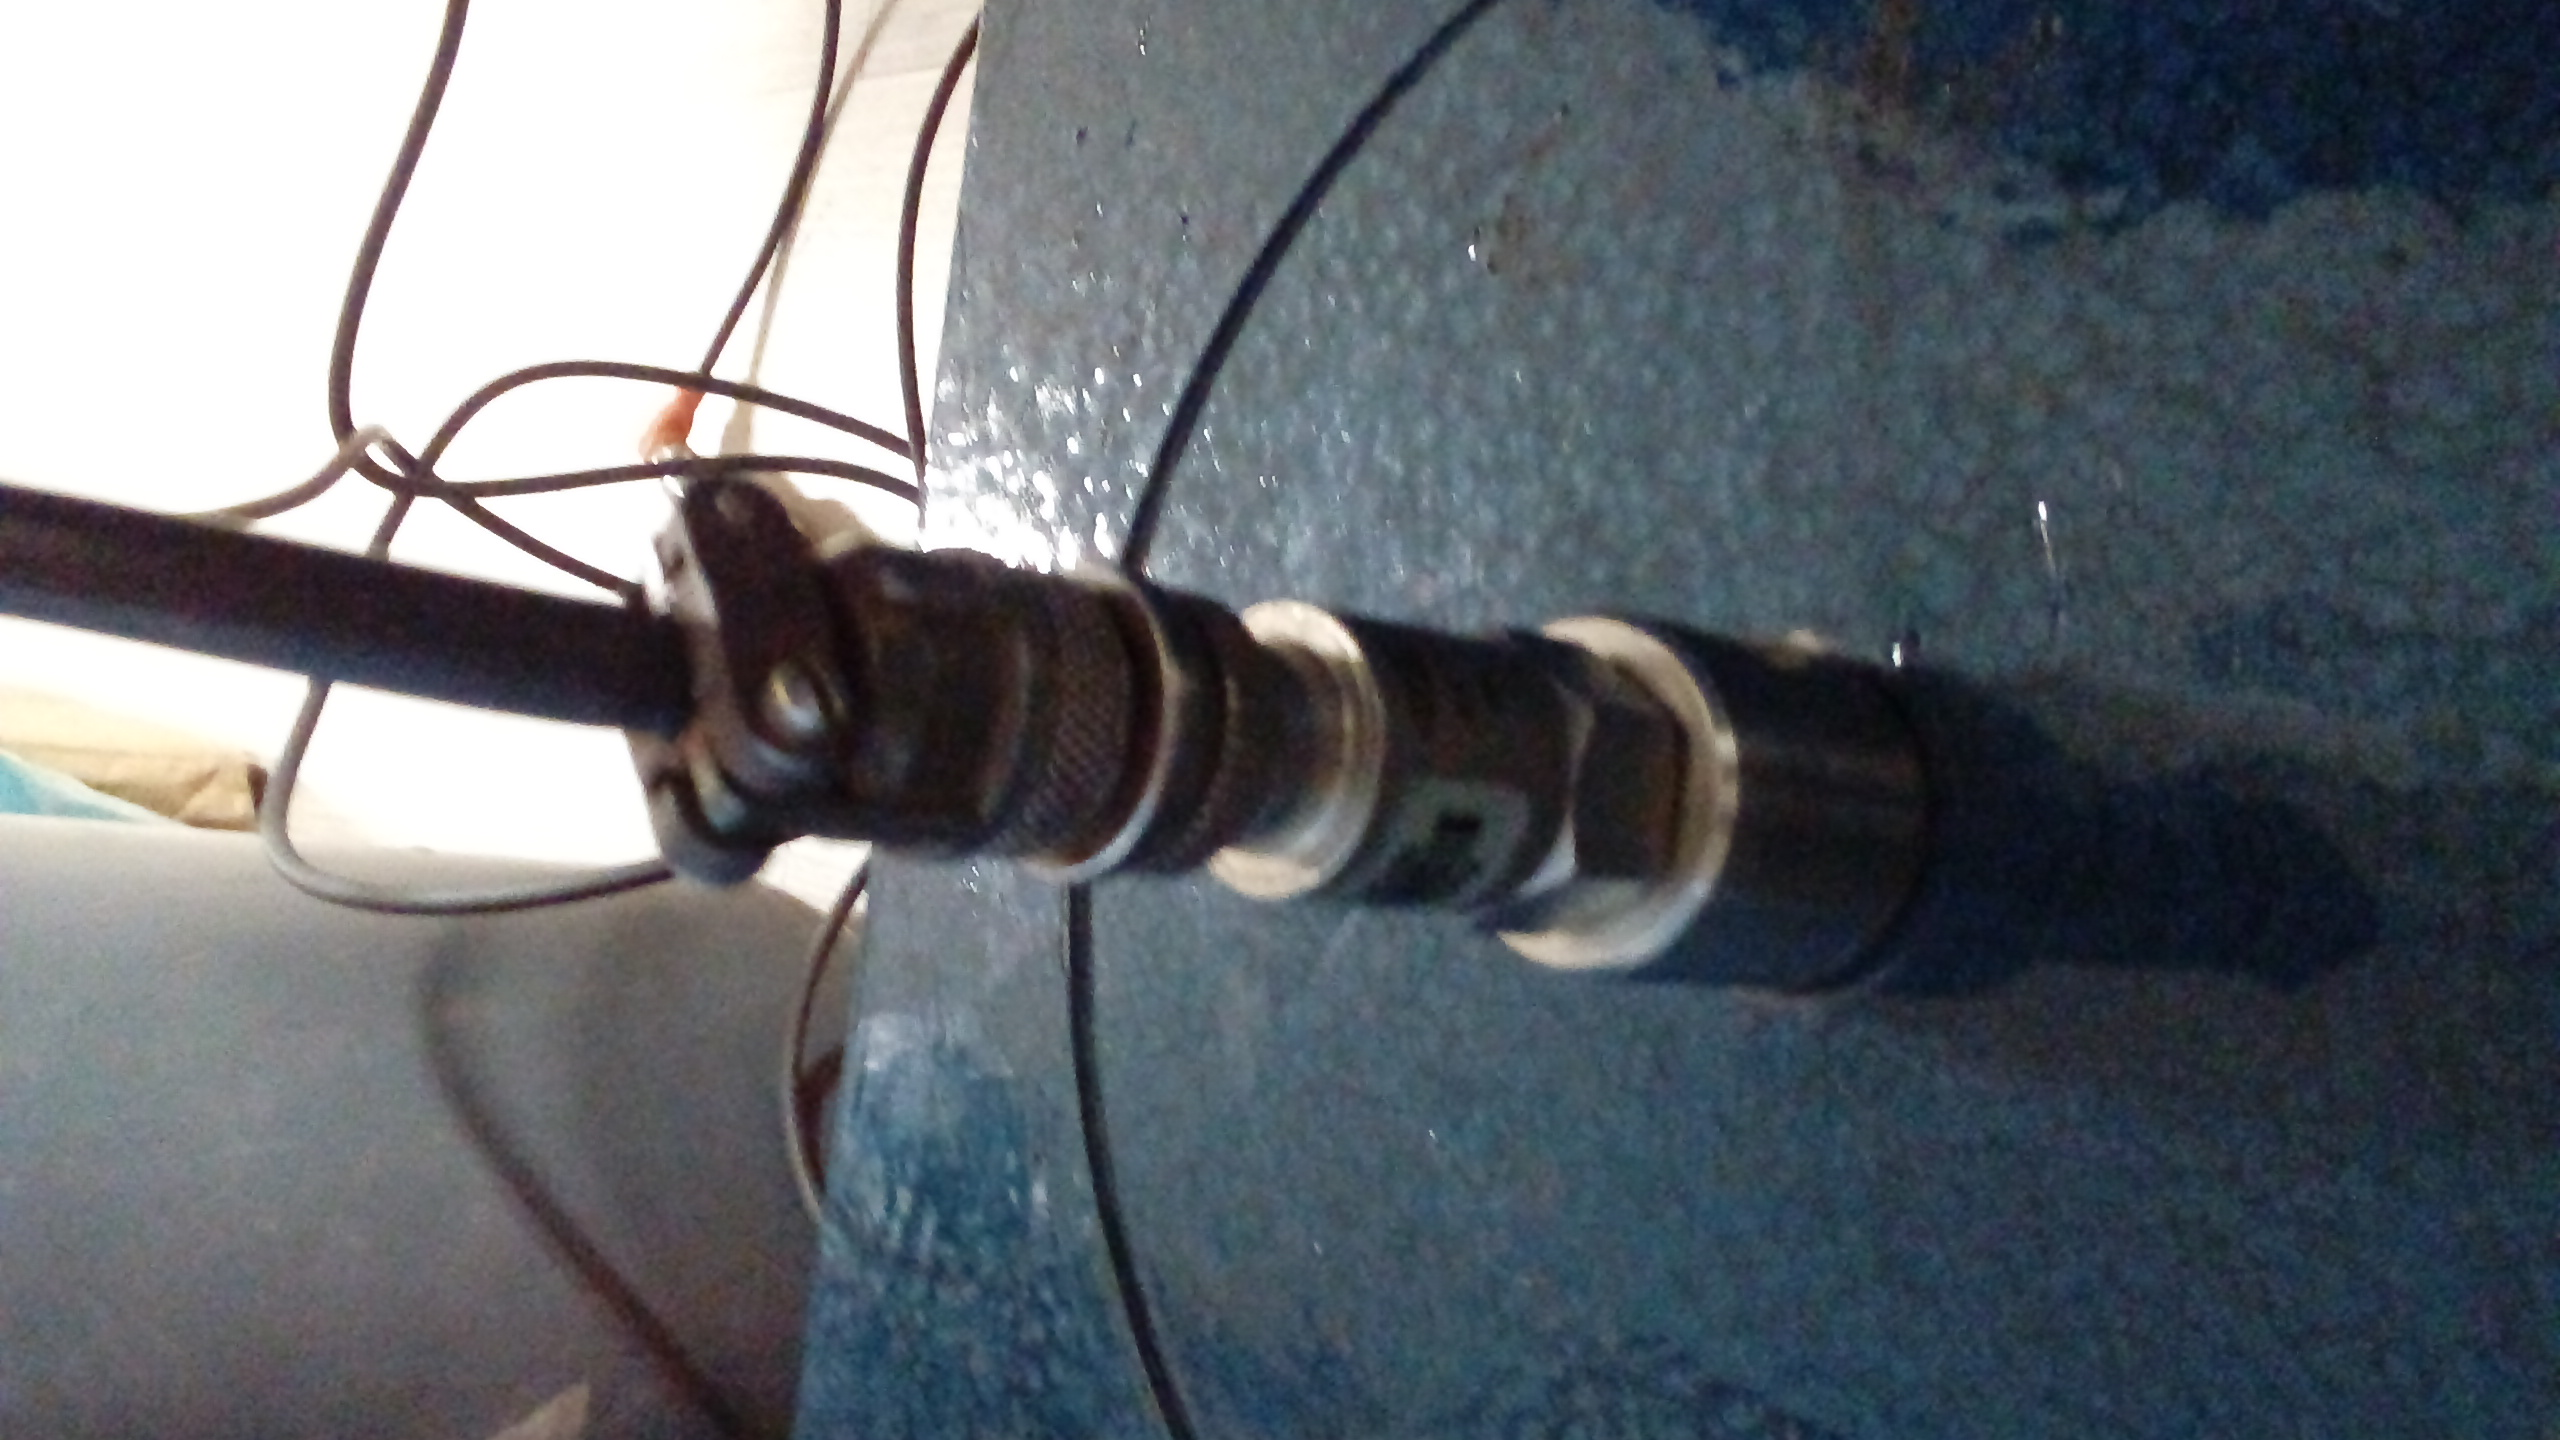
\includegraphics[width = \linewidth, angle = 270, origin = c]{../Fotos/accVertical.jpg}
				\caption{Posição do acelerômetro na parte superior da peneira}
				\label{fig:accNaVertical}
			\end{minipage}
			\hfill\vline\hfill
			\begin{minipage}{0.4\linewidth}
				\centering
				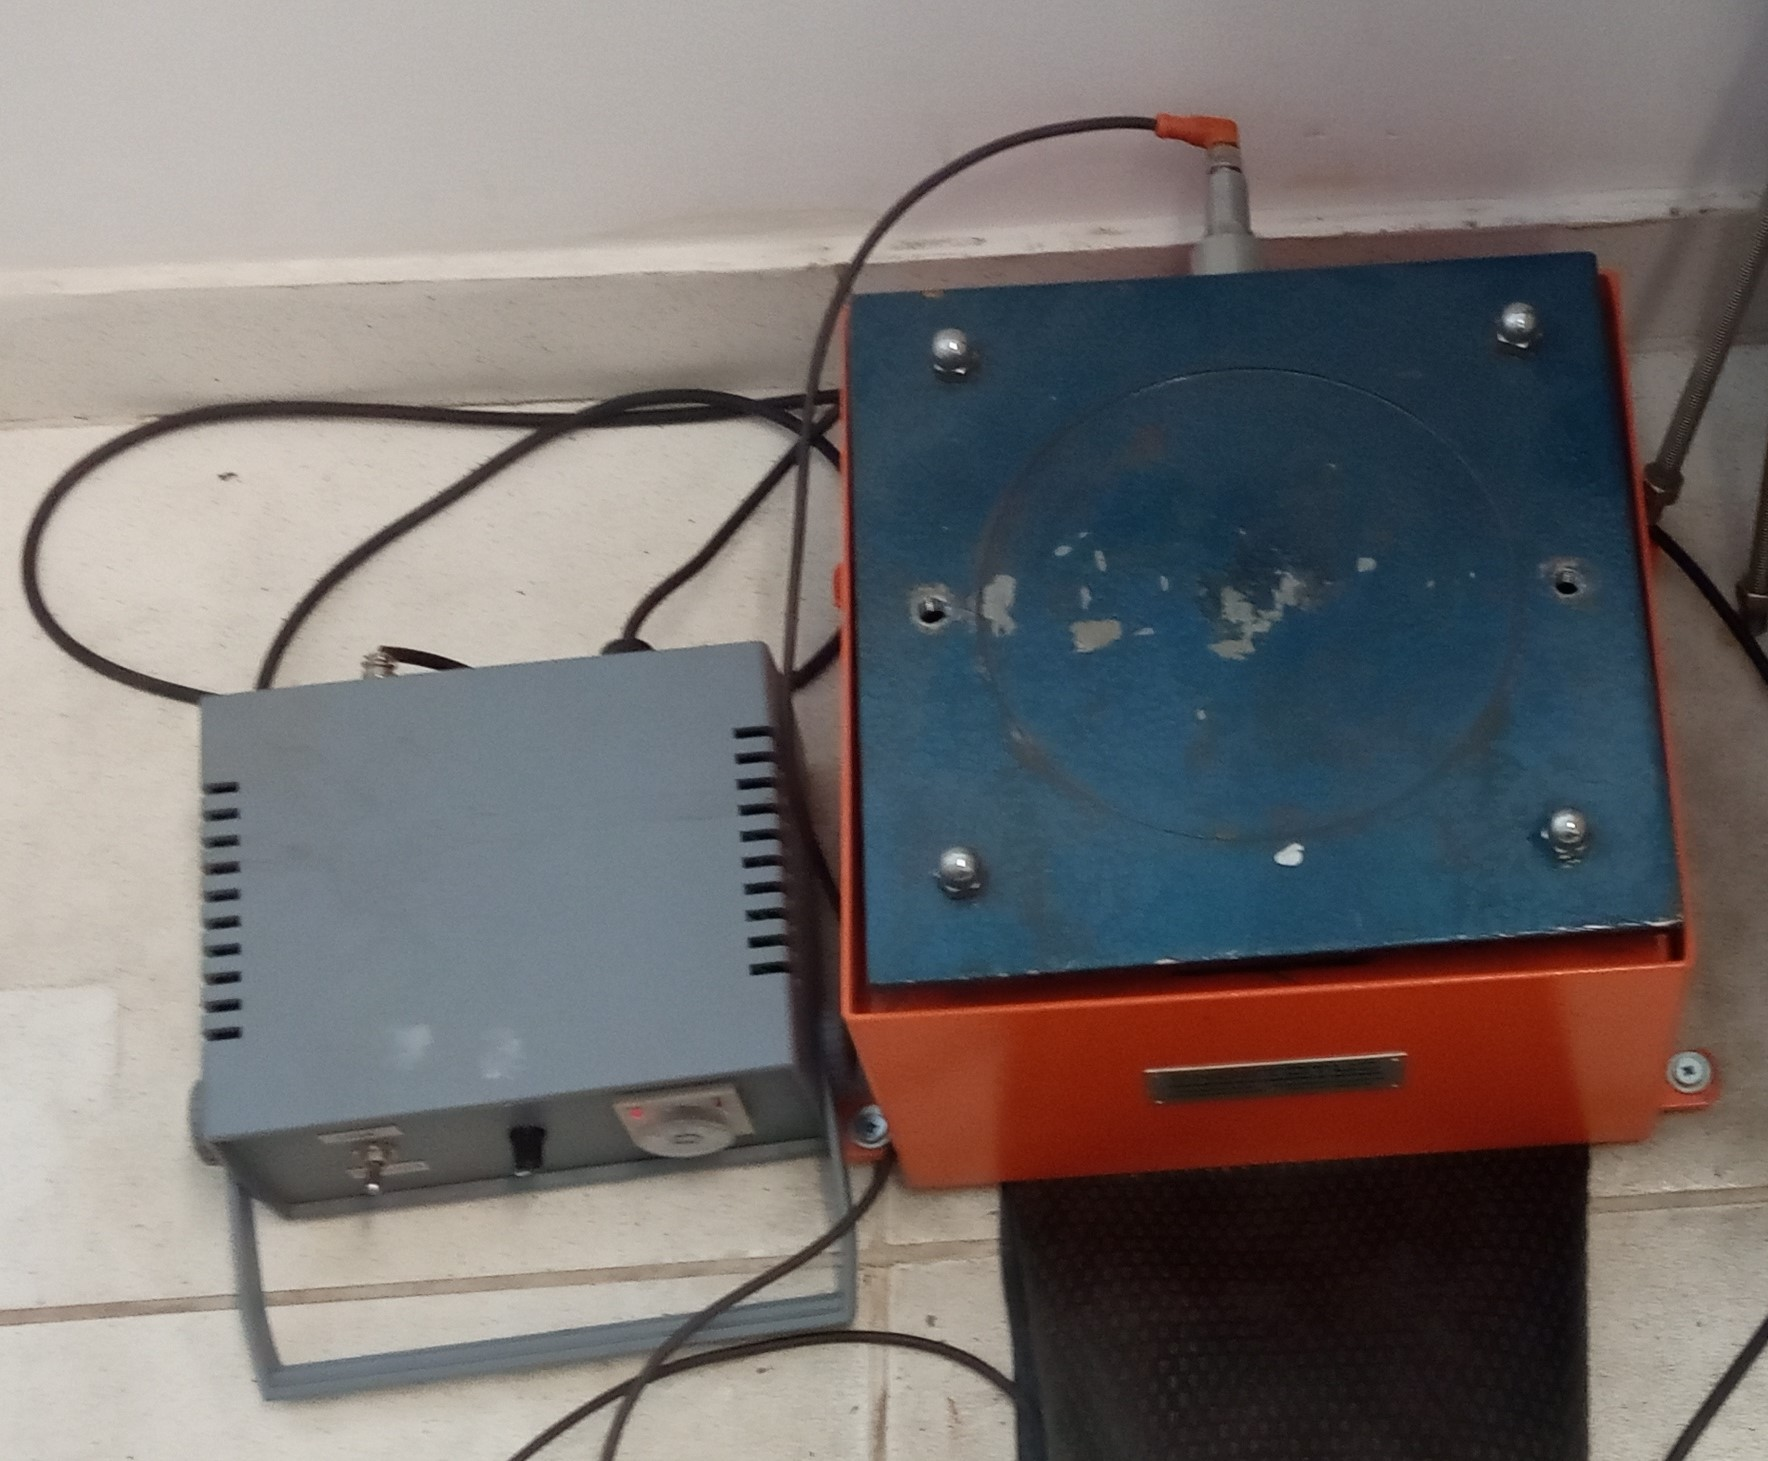
\includegraphics[width = \linewidth]{../Fotos/peneiraAccLateral.jpg}
				\caption{Posição do acelerômetro na lateral da peneira}
				\label{fig:accNaLateral}
			\end{minipage}
		\end{figure}

		Em um segundo momento, realizou-se os mesmos ensaios para o sistema de aquisição desenvolvido, realizando-se ambas medições por 10 segundos, como apresentado na Figura ~\ref{fig:daqIepe}.

		\begin{figure}[H]
			\centering
			\begin{minipage}{0.4\linewidth}
				\centering
				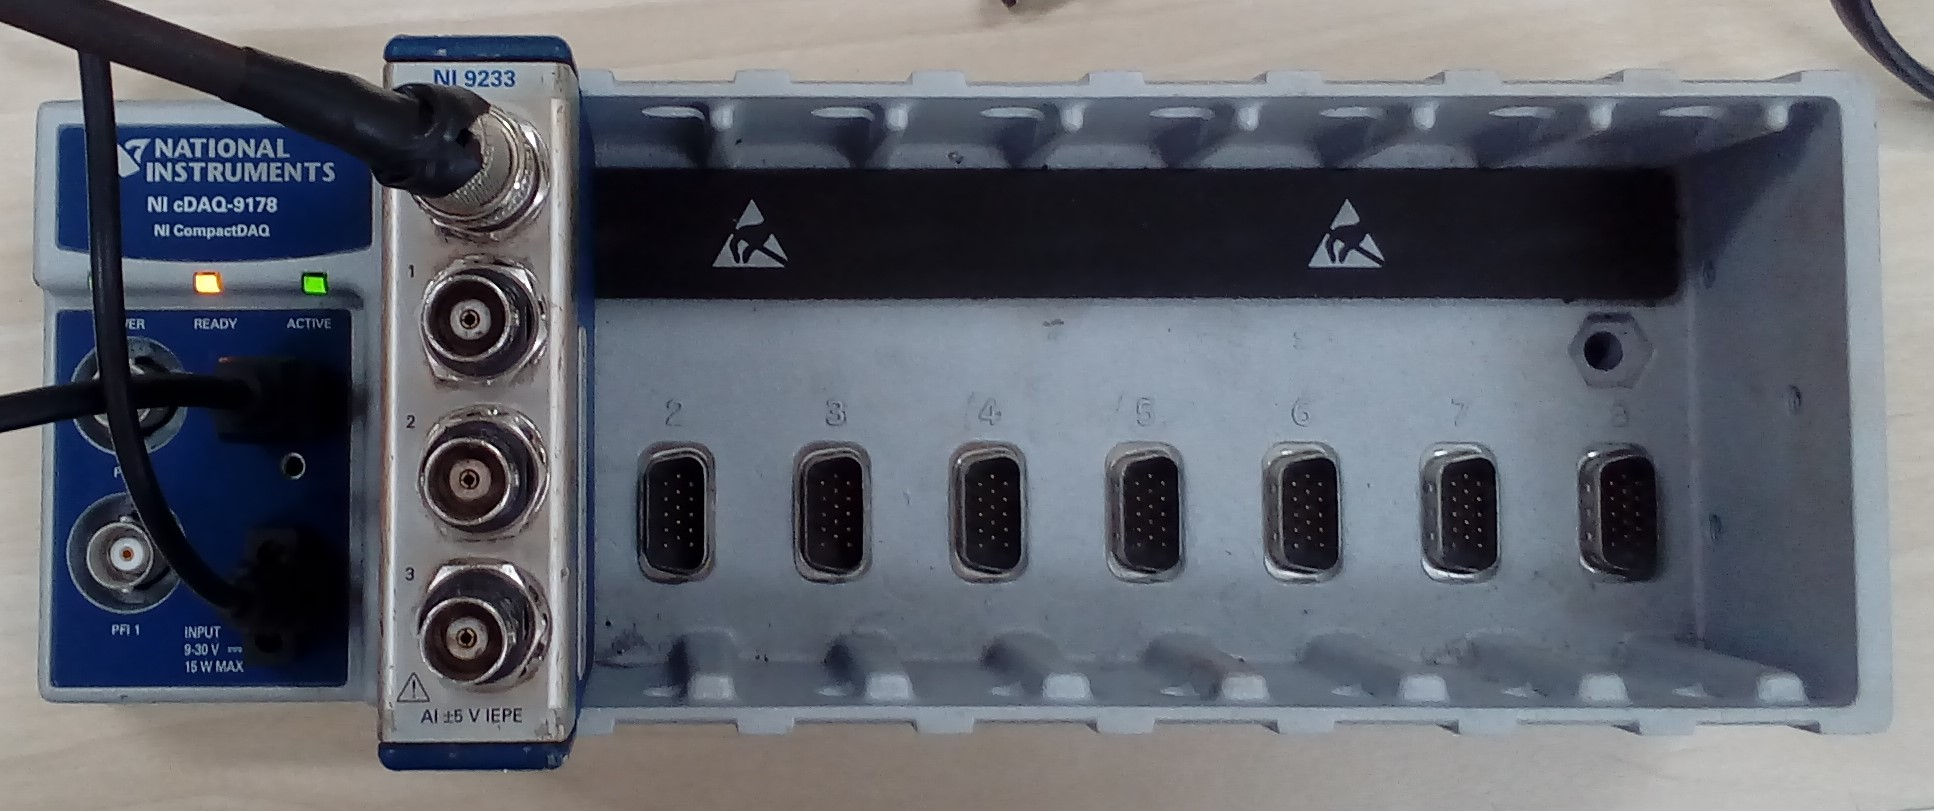
\includegraphics[width = \linewidth]{../Fotos/cdaq.jpg}
				\caption{Sistema de aquisição NI}
				\label{fig:modulosNI}
			\end{minipage}
			\hfill\vline\hfill
			\begin{minipage}{0.4\linewidth}
				\centering
				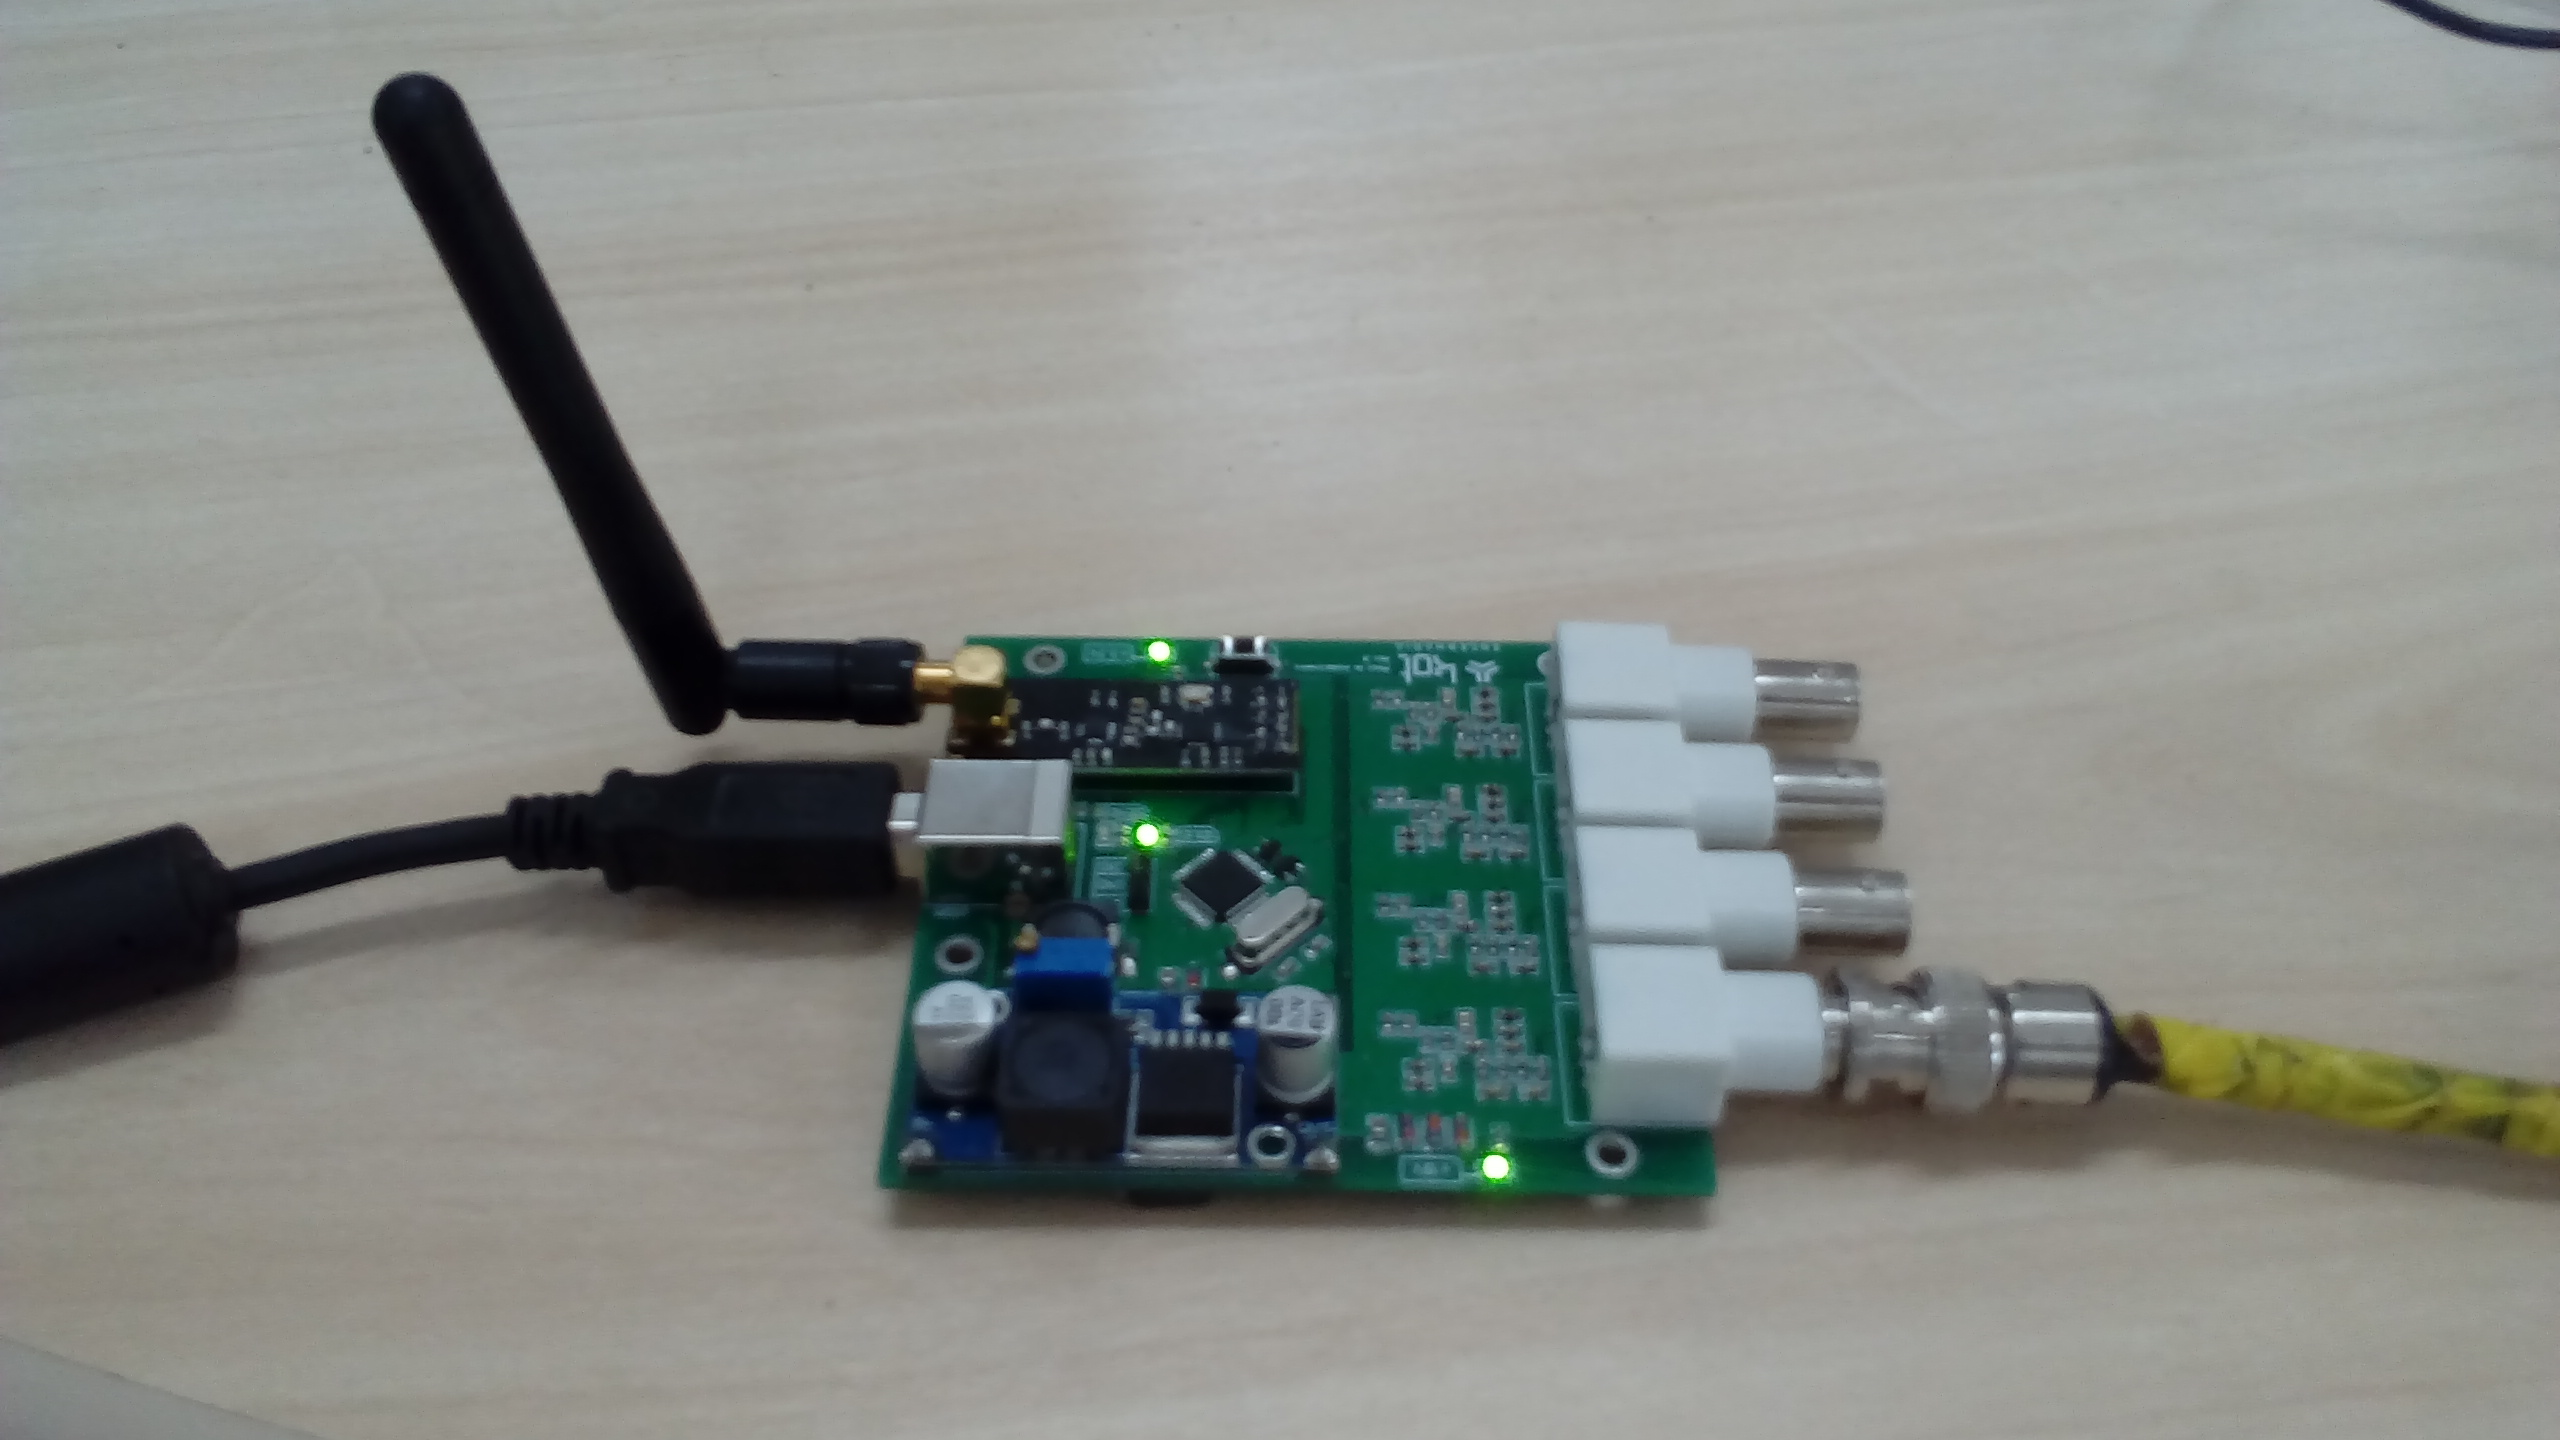
\includegraphics[width = \linewidth]{../Fotos/DAqIEPE.jpg}
				\caption{Sistema de aquisição desenvolvido}
				\label{fig:daqIepe}
			\end{minipage}
		\end{figure}

		Para a análise dos dados, utilizou-se o \textit{software} SignalExpress da National Instruments\textsuperscript{TM}, cedido sob licença da empresa supervisora. Por meio desse \textit{software}, aplicou-se filtros digitais de forma a retirar os sinais fora da banda de interesse. A Figura ~\ref{fig:ni4g} apresenta o sinal de aceleração vertical obtido pelo sistema de aquisição NI-9234 e seu espectro em frequência. O sinal aquisitado pelo sistema desenvolvido é apresentado na Figura ~\ref{fig:kot4g}.

		\begin{figure}[!ht]
			\centering
			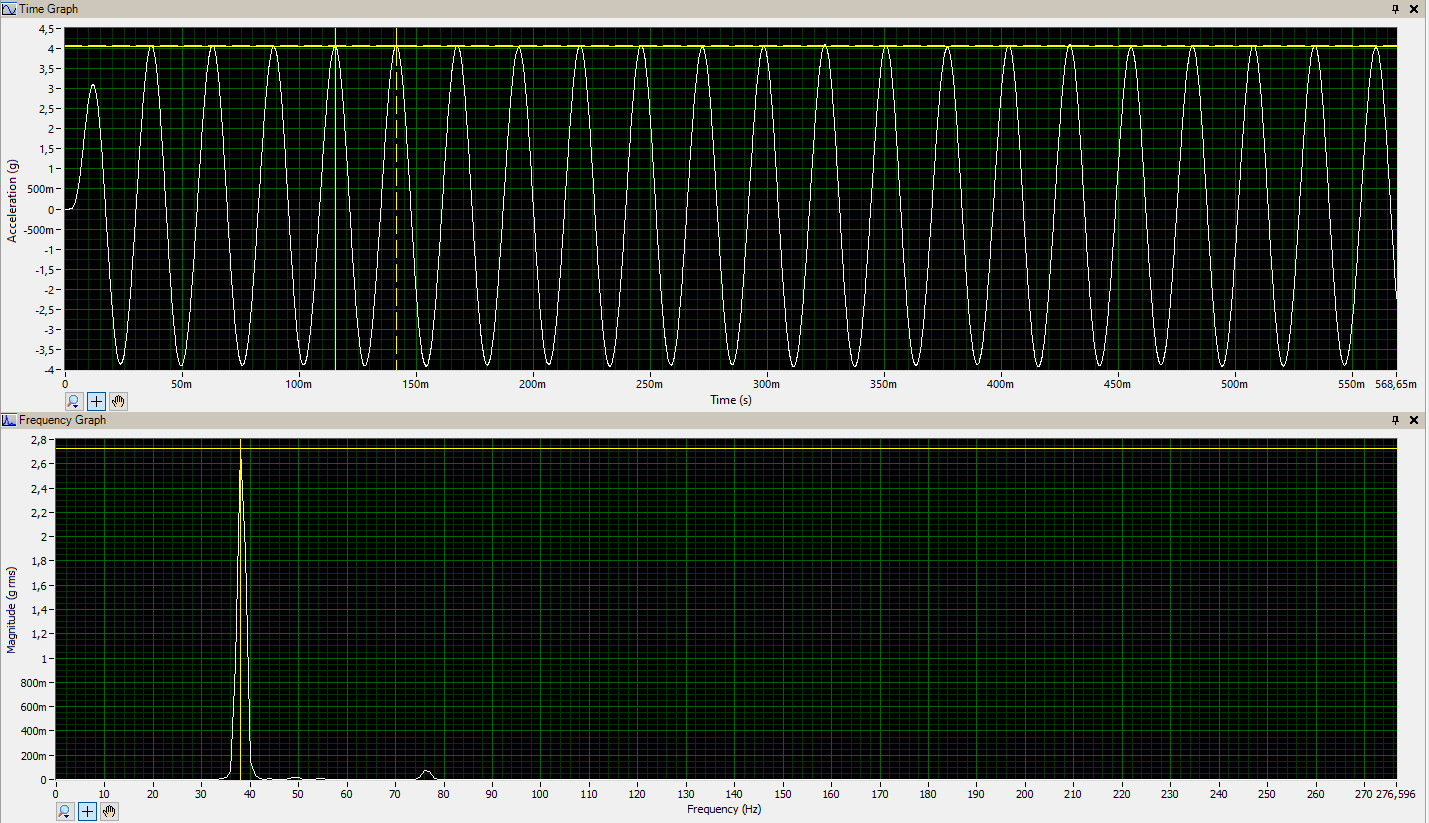
\includegraphics[width=\linewidth]{../Fotos/ni4g.png}
			\caption{Resultados da medição pelo sistema NI-9234 para o ensaio de aceleração vertical}
			\label{fig:ni4g}
		\end{figure}

		\begin{figure}[!ht]
			\centering
			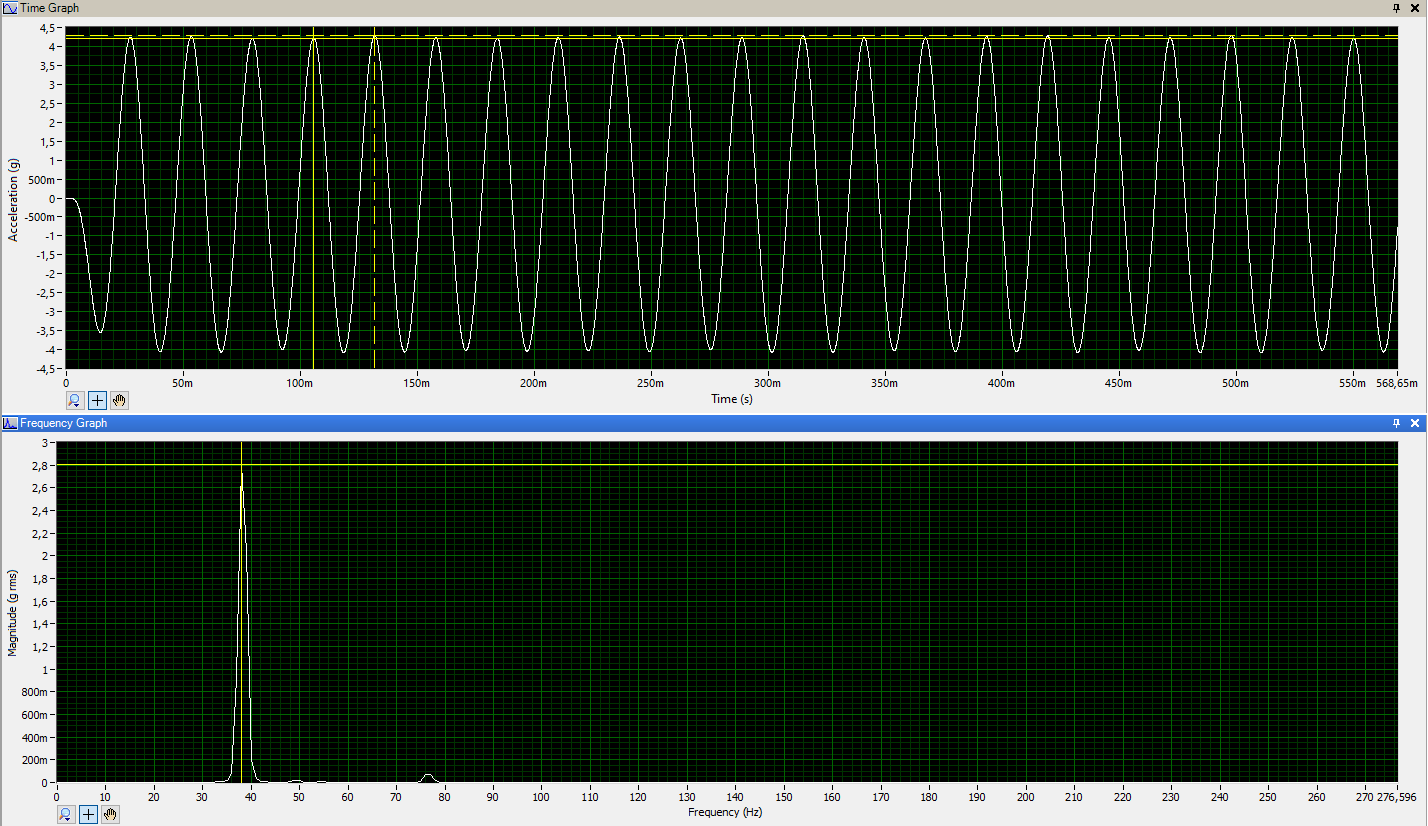
\includegraphics[width=\linewidth]{../Fotos/kot4g.png}
			\caption{Resultados da medição pelo sistema desenvolvido para o ensaio de aceleração vertical}
			\label{fig:kot4g}
		\end{figure}

		Comparando-se as Figuras ~\ref{fig:ni4g} e ~\ref{fig:kot4g}, pode-se notar que os valores em frequência e amplitude dos sinais ficaram próximos nos dois sistemas de aquisição: aproximadamente $4g$ e $38Hz$. O NI-9234 mediu valores de $4,0g$ enquanto o sistema de aquisição desenvolvido obteve até $4,13g$.

		As Figuras ~\ref{fig:ni200mg} e ~\ref{fig:kot200mg} apresentam os sinais obtidos para a medição com o acelerômetro na lateral da peneira.

		\begin{figure}[!ht]
			\centering
			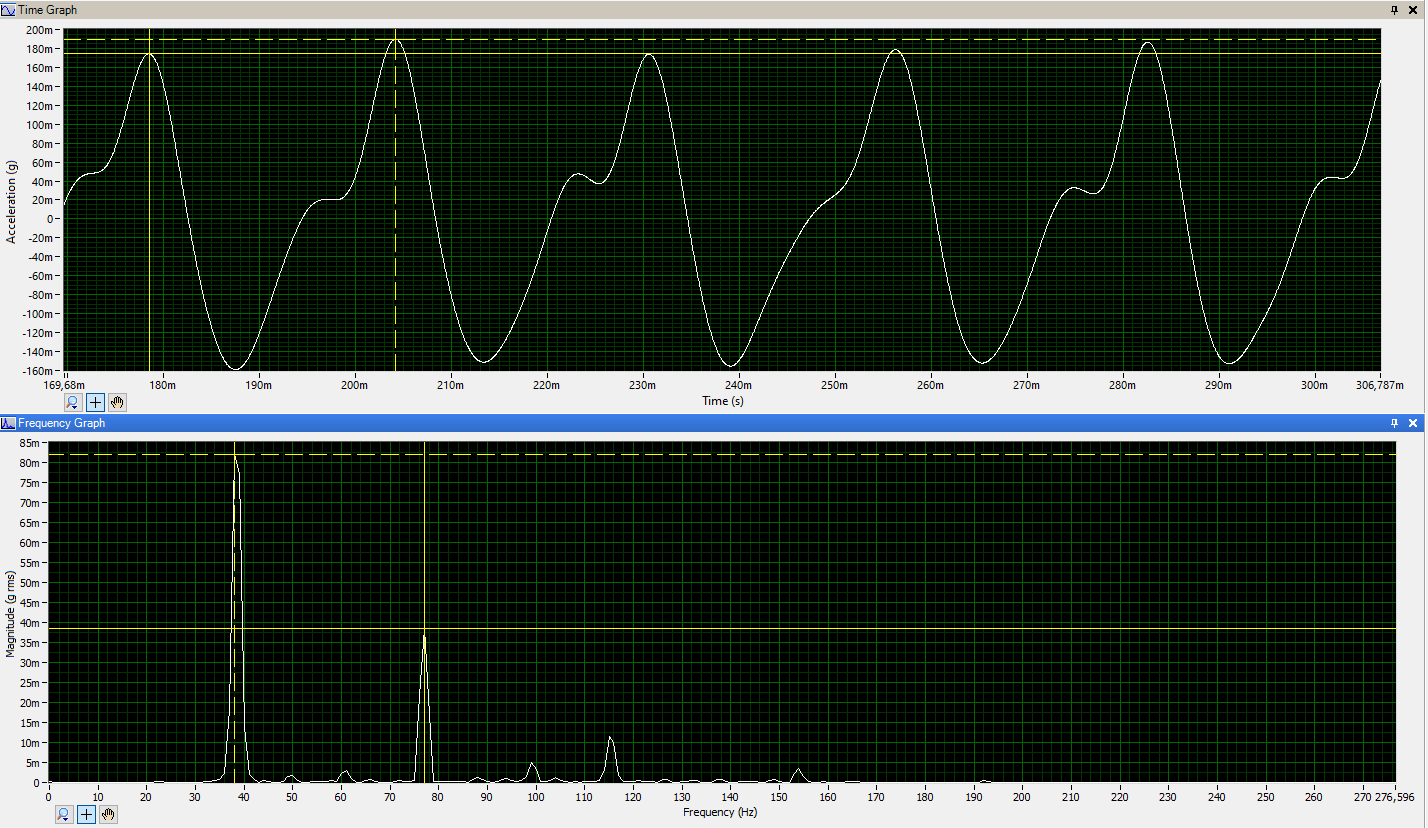
\includegraphics[width=\linewidth]{../Fotos/ni200mg.png}
			\caption{Resultados da medição pelo sistema NI-9234 para o ensaio de aceleração lateral}
			\label{fig:ni200mg}
		\end{figure}

		\begin{figure}[!ht]
			\centering
			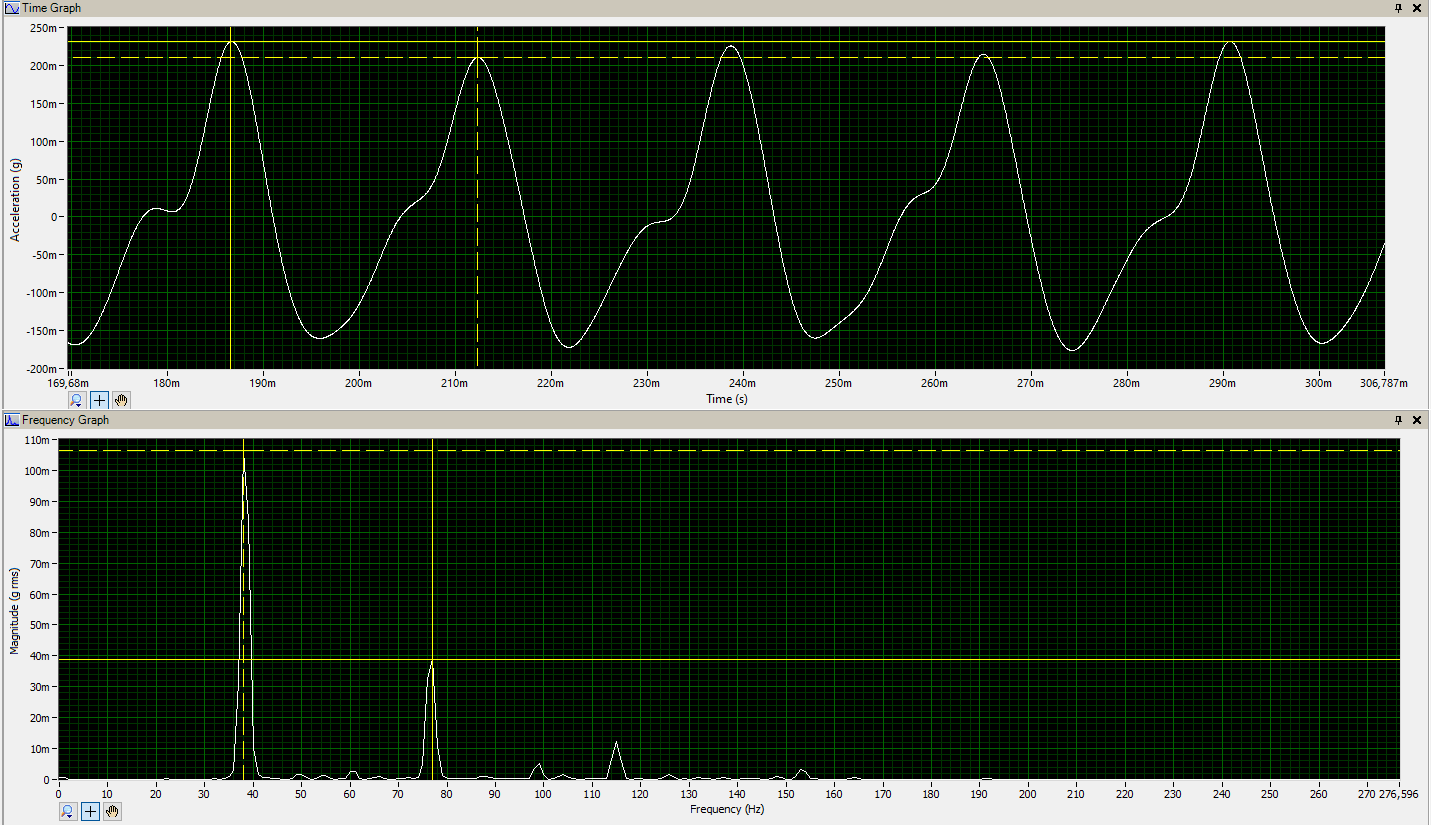
\includegraphics[width=\linewidth]{../Fotos/kot200mg.png}
			\caption{Resultados da medição pelo sistema desenvolvido para o ensaio de aceleração lateral}
			\label{fig:kot200mg}
		\end{figure}

		Comparando-se as Figuras ~\ref{fig:ni200mg} e ~\ref{fig:kot200mg}, pode-se notar que os valores de aceleração ficaram entre $170$ e $190mg$ no sistema de aquisição NI-9234, enquanto a aceleração obtida pelo sistema desenvolvido oscilou entre $210$ e $230mg$. Analisando o espectro de frequência, ambas medições obtiveram valores próximos de frequência, com valores de amplitude um pouco diferentes na frequência de $38Hz$.

		É interessante notar que a diferença entre os valores obtidos pelos dois sistemas de aquisição não é constante ao longo da faixa de medição. Enquanto para valores de referência de $4g$ obteve-se uma variação entre medições de $130mg$ ou $3,25\%$, as medições para menores vibrações para valores de referência de $200mg$ variaram $40mg$ ou $20\%$. Como já explicitado nesta monografia, uma medição de $4g$ ou $4,13g$ não possui impacto na avaliação do estado de uma máquina como uma peneira. Apenas variações maiores, na ordem de \textit{1g} impactariam na medição. Com isso, pode-se dizer que o sistema possui um bom desempenho quando referenciado ao sistema de aquisição NI-9234 e atende às necessidades propostas. Os demais canais foram testados e todos apresentaram comportamento semelhante aos valores já apresentados.

		Para analisar o alcance de envio do sistema de aquisição, realizou-se testes na rua e em ambientes fechados, ambos com área livre entre o emissor e o receptor. Consegue-se receber os dados sem perda de pacotes com distâncias de até 70 metros. Até 100 metros, cerca de $1\%$ dos pacotes são perdidos. Acima dessa distância a comunicação fica instável e não confiável.

%#Endregion

% ----------------------------------------------------------
%#Region Capítulo 5 - Conclusões
% ----------------------------------------------------------
\chapter{Conclusões}

	O desenvolvimento da monografia possibilitou uma experiência imersiva com
	projetos de sistemas de aquisição de dados aplicados à problemas
	reais da indústria. Foi necessário aplicar conhecimento
	interdisciplinar entre teoria de comunicações, processamento de
	sinais, sistemas de processadores de periféricos e eletrônica
	analógica. O projeto agregou experiência tanto no aspecto
	profissional e técnico quanto no ambiente de trabalho, que valoriza
	o profissional e viabiliza o desenvolvimento de novas tecnologias
	mesmo em um cenário econômico nacional turbulento.

	O projeto ainda deve passar por alguns ensaios para avaliar as reais
	condições de funcionamento. Pode-se considerar que obteve desempenho satisfatório, atendendo
	todas as condições de contorno com margens de segurança.
	
	Como trabalhos futuros, pode-se listar:
	
	\begin{itemize}
		\item Validação de toda a faixa de banda de passagem
		\item Validação do alcance máximo do módulo para diferentes condições ambiente
		\item Algoritmo para retransmissão de dados no caso de perda de pacotes
		\item Otimização das bibliotecas implementadas
		\item Interface de recebimento de dados com possibilidade de parametrização do módulo
	\end{itemize}

%#Endregion

% ---
% Finaliza a parte no bookmark do PDF, para que se inicie o bookmark na raiz
% ---
\bookmarksetup{startatroot}% 
% ---

% ----------------------------------------------------------
% ELEMENTOS PÓS-TEXTUAIS
% ----------------------------------------------------------
\postextual

% ----------------------------------------------------------
% Referências bibliográficas
% ----------------------------------------------------------
% \bibliography{abntex2-modelo-references}
\bibliography{../Bibliografia/bibliografia}

% ----------------------------------------------------------
% Apêndices
% ----------------------------------------------------------

% ---
% Inicia os apêndices
% ---
\begin{apendicesenv}

% Imprime uma página indicando o início dos apêndices
\partapendices

% ----------------------------------------------------------
\chapter{Cálculo do ganho e de bits do ADC}
% ----------------------------------------------------------
	\label{ape:calculoADC}

	A excursão do sinal de $V_{o(av)}$ até $V_{o(max)}$ representa a excursão de aceleração
	de $0g$ a $50g$. Assim, a excursão de 1mg representa um sinal de tensão de:

	\begin{gather*}
		V_{o(1mg)} = \frac{V_{o(max)} - V_{o(av)}}{50000mg}\\
		V_{o(1mg)} = \frac{G\*V_{i(av)} + G\*\frac{V_{i(pp)}}{2} - G\*V_{i(av)}}{50000}\\
		V_{o(1mg)} = \frac{G\*V_{i(pp)}}{100000}\\
		V_{o(1mg)} = 10\*G/100000\\
		V_{o(1mg)} = G/10000
	\end{gather*}

	E $100mg$ representam $100$ vezes o valor anterior. Logo:
	\begin{gather*}
		V_{o(100mg)} =100\*V_{o(1mg)}\\
		V_{o(100mg)} =100\*G/10000\\
		V_{o(100mg)} =G/100
	\end{gather*}
	Percebe-se que o valor da tensão de saída pode ser escrita em função apenas do ganho, podendo esta variar entre os valores nominais do transdutor	de $10V$ a $14V$. Isso se dá uma vez que realiza-se a correção do \textit{offset}, tornando $V_{o(100mg)}$ um valor diferencial. Assim, o valor da tensão depende apenas do ganho.

	Por sua vez, o ganho é dado por:
	\begin{gather*}
		G = V_{o(max)}/V_{i(max)}
	\end{gather*}
	Em que $V_{o(max)}$ é a tensão de alimentação do conversor ADC e $V_{i(max)}$ é
	$19V$. Da expressão do número de \textit{bits} do ADC, têm-se que:
	\begin{gather*}
		LSB = \frac{V_{o(max)}}{2^n}\\
		ou\\
		V_{o(max)} = LSB\times 2^n
	\end{gather*}
	em que:\\
	\textit{LSB} (\textit{Least Significant Bit}) é a resolução do ADC;\\
	\textit{n} é o número de \textit{bits} do ADC.\\

	Como já citado, a menor resolução da grandeza a ser lida deve ser de
	$100mg$. Sendo a sensibilidade do sensor $100mV/g$, então $100mg$
	correspondem a $10mV$ de excursão na tensão de entrada. Dessa forma,
	pode-se escrever LSB em função da mínima resolução desejada.
	\begin{gather*}
		LSB = 10\times 10^{-3}\times G
	\end{gather*}
	Substituindo na equação do ganho:
	\begin{gather*}
		G = V_{o(max)}/V_{i(max)}\\
		G = \frac{LSB\times 2^n}{V_{i(max)}}\\
		G = \frac{G\times 10\times 10^{-3}\times 2^n}{V_{i(max)}}\\
		1 = \frac{10\times 10^{-3}\*2^n}{V_{i(max)}}\\
		2^n = \frac{V_{i(max)}}{10\times 10^{-3}}\\
		n = log_2\left( \frac{V_{i(max)}}{10\times 10^{-3}} \right) = log_2\left( \frac{19}{10^{-2}}\right)\\
		n = 10,89
	\end{gather*}
	Como o número de \textit{bits} do conversor ADC deve ser um número inteiro e múltiplo de $2$, \textit{n}
	deve ser minimamente $12$ \textit{bits} para atender às condições de contorno. É
	interessante pontuar que o número de \textit{bits} independe da tensão de
	alimentação do conversor ADC, seja ela $3,3V$ ou $5V$. E, consequentemente,
	independe do ganho $G$.

	Para o cálculo do ganho $G$ admite-se o pior caso, ou seja, um sinal médio
	de saída de $14V$ com excursão positiva máxima, gerando um sinal de $19V$. O
	ganho deve ser tal que $19V$ seja atenuado para $5V$ ou $3,3V$. Para isso, o
	ganho deve ser de, respectivamente, $0,263V/V$ ou $0,1737V/V$.

% ----------------------------------------------------------
\chapter{Cálculo dos componentes da fonte de corrente}
% ----------------------------------------------------------
\label{ape:calculoCorrente}

	Admitindo uma impedância de medição infinita e alpha dos transistores
	$\alpha\simeq1$, a corrente entregue ao sensor \textit{IEPE} será dada por:
	\begin{gather*}
		I_s = V_{be}/R_1
	\end{gather*}
	Assim, considerando $V_{be}$ aproximadamente constante e igual a $0,7V$ e
	$I_s = 4mA$:
	\begin{gather*}
		R_1 = V_{be}/I_s = 170\Omega
	\end{gather*}
	O resistor $R_2$ garante a polarização de ambos transistores. A
	corrente necessária para polarizar o $Q_1$ será aproximadamente a
	corrente total que passa pelo resistor $R_2$. Segundo o
	\textit{datasheet} do transistor PNP BC857, para $V_{be} = 0,7V$
	tem-se $I_c = 2mA$. $R_2$ possui queda de tensão de $19V -
	2\*V_{be}$. Assim:
	\begin{gather*}
		R_2 = \frac{19 - 2\*V_{be}}{0,002} = 8k88\Omega
	\end{gather*}
	Após montar e simular o circuito, utilizando o \textit{software}
	LTSpice, foi possível realizar um ajuste fino para reduzir a
	corrente de polarização do transistor para cerca de $350\mu A$,
	fazendo com que ambos $V_{be}s$ ficassem em torno de $0,6V$. Assim,
	o novo valor de $R_1$ e $R_2$, aproximado para valores comerciais,
	são:
	\begin{gather*}
		R_1 = 0,6/0,004 = 150\Omega\\
		R_2 = \frac{19-2\times 0,6}{0,00035} = 51k\Omega
	\end{gather*}

	A fonte de corrente que alimenta o sensor IEPE deve possuir
	corrente de saída de $2mA$ a $10mA$. Como o valor da corrente
	escolhido é um valor intermediário, $4mA$, os resistores da
	fonte de corrente não precisam ter valores precisos. Resistores
	de 5\% podem ser usados sem influenciar nos resultados.

% ----------------------------------------------------------
\chapter{Dimensionamento do conversor DC/DC \textit{boost}}
% ----------------------------------------------------------
\label{ape:calculoBoost}

	Para elevar a tensão, utiliza-se uma fonte chaveada tipo
	\textit{boost}. De forma a manter a uma alta eficiência do
	\textit{boost} e não trabalhar com uma tensão muito próxima do
	limite inferior do acelerômetro, a tensão de alimentação escolhida foi de $19V$.
	A corrente total que a fonte de 19V deve fornecer é dada por:
	\begin{gather*}
		I_{total} = 4\* \left(I_{FAA} + I_{FonteCorrente}\right)
	\end{gather*}
	O valor é multiplicado por quatro pois são quatro canais de medição. A corrente do FAA
	é basicamente a corrente consumida pelos amplificadores
	operacionais que, segundo o \textit{datasheet} do OP07CDR \cite{op07c}, é de
	menos de $1mA$ para tensões de alimentação superiores a
	aproximadamente $11V$. Assim, como cada FAA possui quatro OP07CDR,
	o consumo do FAA é de $4\times 1mA =  4mA$.

	As fontes de corrente consomem $4mA$ da polarização do sensor
	mais a corrente que passa pelo resistor de polarização $R_2$ da Figura ~\ref{fig:topologiaFonteCorrenteValores}.
	Assim, cada filtro consome aproximadamente $4,3mA$. Então:
	\begin{gather*}
		I_{total} = 4\* \left(4mA + 4,3mA\right) = 33,2mA.
	\end{gather*}

	Assim, a fonte \textit{boost} deve ser capaz de elevar a tensão
	de $5V$ para $19V$ e fornecer uma corrente de $60mA$, aplicando uma
	margem de segurança. Devido ao baixo custo e por atender às
	especificações do projeto, optou-se pelo módulo \textit{boost}
	XL6009. Trata-se de uma fonte chaveada elevadora de tensão com
	capacidade de regular a tensão de saída por meio de um
	\textit{trimpot} até $32V$ e capacidade nominal de corrente de $4A$.

\end{apendicesenv}
% ---

% ----------------------------------------------------------
% Anexos
% ----------------------------------------------------------

% ---
% Inicia os anexos
% ---
% \begin{anexosenv}

% % Imprime uma página indicando o início dos anexos
% \partanexos

% % ---
% \chapter{Morbi ultrices rutrum lorem}
% % ---
% %\lipsum[60]

% % ---
% \chapter{Cras non urna sed feugiat cum sociis natoque penatibus}
% % ---
% %\lipsum[61-63]

% % ---
% \chapter{Fusce facilisis lacinia dui}
% ---
%\lipsum[64-65]

% \end{anexosenv}

\end{document}
